% Relaxation dispersion.
%%%%%%%%%%%%%%%%%%%%%%%%

\chapter[Relaxation dispersion]{The analysis of relaxation dispersion} \label{ch: relax-disp}
\index{relaxation dispersion|textbf}

\begin{figure*}[h]
  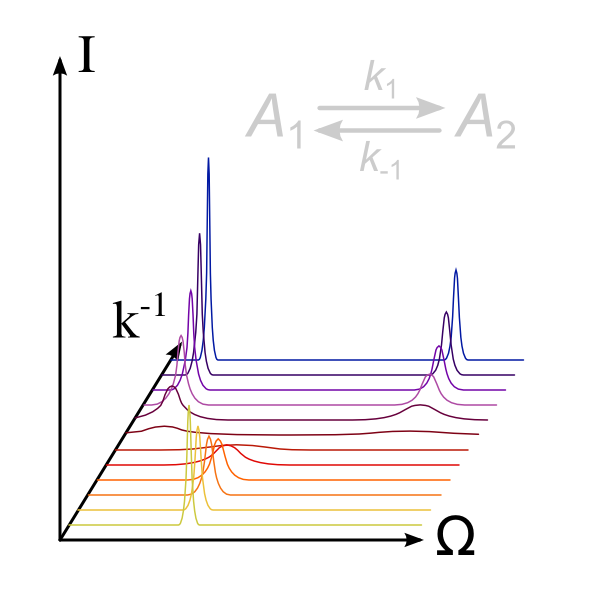
\includegraphics[width=5cm, bb=0 0 1701 1701]{graphics/analyses/relax_disp_600x600}
\end{figure*}


% Introduction.
%%%%%%%%%%%%%%%

\section{Introduction to relaxation dispersion}

Relaxation dispersion is the experimental modulation of chemical exchange relaxation.
For the $\Ronerho$-type experiment in which the nucleus of interest is spin-locked, either the spin-lock field strength or the offset between the spin-lock pulse and the chemical shift of the spins is used to modulate the exchange.
For the CPMG-type experiment, varying the time between the pulses modules the exchange.
Both experiment types are handled by relax.

The primary reference for the relaxation dispersion implemented in relax is:
\begin{itemize}
  \item \bibentry{Morin14}
\end{itemize}

For other citations, please see the citation chapter on page~\pageref{ch: citations}.


% The models.
%~~~~~~~~~~~~

\subsection{The modelling of dispersion data}

For a system under the influence of chemical exchange, the evolution of the transverse magnetisation is given by the \citet{Bloch46} equations as modified by \citet{McConnell58} for chemical exchange -- the Bloch-McConnell equations.
For a two state exchange jumping between states A and B, the equation is:

\begin{equation} \label{eq: Bloch-McConnell}
    \frac{d}{dt} \left[ 
        \begin{array}{c}
            M_A^+(t) \\
            M_B^+(t)
        \end{array}
    \right] = \left[
        \begin{array}{cc}
            -i\Omega_A-\RtwozeroA-\pB\kex & \pA\kex \\
            \pB\kex & -i\Omega_B-\RtwozeroB-\pA\kex \\
        \end{array}
    \right] \left[
        \begin{array}{c}
            M_A^+(t) \\
            M_B^+(t)
        \end{array}
    \right] .
\end{equation}

The analytic or closed-form frequency-domain solution for this equation however remains intractable.
Solutions can nevertheless be found by either making assumptions or restrictions about the exchange process and then analytically solving~\ref{eq: Bloch-McConnell} or by finding numeric solutions.
The modelling of relaxation dispersion data can hence be categorised into these two distinct methodologies:
\begin{description}
  \item[Analytical models:]\index{relaxation dispersion!Analytical model}  Optimisation of models based on analytical, closed-form expressions derived from the Bloch-McConnell equations subject to certain conditions (see Section~\ref{sect: dispersion: analytic CPMG models} on page~\pageref{sect: dispersion: analytic CPMG models} and Section~\ref{sect: dispersion: analytic R1rho models} on page~\pageref{sect: dispersion: analytic R1rho models}).
  \item[Numerical models:]\index{relaxation dispersion!Numerical model}  Optimisation of models based on numerically solving the Bloch-McConnell equations (see Section~\ref{sect: dispersion: numeric CPMG models} on page~\pageref{sect: dispersion: numeric CPMG models} and Section~\ref{sect: dispersion: numeric R1rho models} on page~\pageref{sect: dispersion: numeric R1rho models}).
\end{description}



% Implemented models.
%~~~~~~~~~~~~~~~~~~~~

\subsection{Implemented models}
\label{sect: dispersion: implemented models}

A number of analytic and numeric models are supported within relax.
These cover single quantum (SQ) CPMG-type, combined proton-heteronuclear single quantum (SQ), zero quantum (ZQ), double quantum (DQ) and multi quantum (MQ) CPMG-type experiments, and $\Ronerho$-type.
If the model you are interested in is not available, please see Section~\ref{sect: dispersion: model tutorial} on page~\pageref{sect: dispersion: model tutorial} for how you can add new models to relax.

Models which are independent of the experiment type include:
\begin{description}
  \item[`R2eff':]\index{relaxation dispersion!R2eff model}  This is the model used to determine the $\Rtwoeff$ or $\Ronerho$ values and errors required as the base data for all other models.
    See Section~\ref{sect: dispersion: R2eff model} on page~\pageref{sect: dispersion: R2eff model}.
  \item[`No Rex':]\index{relaxation dispersion!No Rex model}  This is the model for no chemical exchange being present.
    See Section~\ref{sect: dispersion: No Rex model} on page~\pageref{sect: dispersion: No Rex model}.
\end{description}


For the SQ CPMG-type experiments, the analytic models currently supported are:
\begin{description}
  \item[`LM63':]\index{relaxation dispersion!LM63 model}  The original \citet{LuzMeiboom63} 2-site fast exchange equation with parameters $\{\Rtwozero, \dots, \Phiex, \kex\}$.
    See Section~\ref{sect: dispersion: LM63 model} on page~\pageref{sect: dispersion: LM63 model}.
  \item[`LM63 3-site':]\index{relaxation dispersion!LM63 3-site model}  The original \citet{LuzMeiboom63} 3-site fast exchange equation with parameters $\{\Rtwozero, \dots, \PhiexB, \kB, \PhiexC, \kC\}$.
    The equations of \citet{OConnell09} can be used to approximately convert the parameters $\{\PhiexB, \kB, \PhiexC, \kC\}$ to more biologically relevant parameters.
    See Section~\ref{sect: dispersion: LM63 3-site model} on page~\pageref{sect: dispersion: LM63 3-site model}.
  \item[`CR72':]\index{relaxation dispersion!CR72 model}  The reduced \citet{CarverRichards72} 2-site equation for most time scales whereby the simplification $\RtwozeroA = \RtwozeroB$ is assumed.
    It has the parameters $\{\Rtwozero, \dots, \pA, \dw, \kex\}$.
    See Section~\ref{sect: dispersion: CR72 model} on page~\pageref{sect: dispersion: CR72 model}.
  \item[`CR72 full':]\index{relaxation dispersion!CR72 full model}  The full \citet{CarverRichards72} 2-site equation for most time scales with parameters $\{\RtwozeroA, \RtwozeroB, \dots, \pA, \dw, \kex\}$.
    See Section~\ref{sect: dispersion: CR72 full model} on page~\pageref{sect: dispersion: CR72 full model}.
  \item[`IT99':]\index{relaxation dispersion!IT99 model}  The \citet{IshimaTorchia99} 2-site model for all time scales with $\pA \gg \pB$ and with parameters $\{\Rtwozero, \dots, \pA, \dw, \tex\}$.
    See Section~\ref{sect: dispersion: IT99 model} on page~\pageref{sect: dispersion: IT99 model}.
  \item[`TSMFK01':]\index{relaxation dispersion!TSMFK01 model}  The \citet{Tollinger01}  2-site very-slow exchange model for time scales within range of microsecond to second time scale.
    Applicable in the limit of slow exchange, when $|\RtwozeroA - \RtwozeroB| \ll \kAB, \kBA \ll 1/\taucpmg$.
    $2*\taucpmg$ is the time between successive 180 degree pulses.
    Parameters are $\{\RtwozeroA, \dots, \dw, \kAB\}$.
    See Section~\ref{sect: dispersion: TSMFK01 model} on page~\pageref{sect: dispersion: TSMFK01 model}.
  \item[`B14':]\index{relaxation dispersion!B14 model}  The reduced \citet{Baldwin2014} 2-site exact solution equation for all time scales whereby the simplification $\RtwozeroA = \RtwozeroB$ is assumed.
    It has the parameters $\{\Rtwozero, \dots, \pA, \dw, \kex\}$.
    See Section~\ref{sect: dispersion: B14 model} on page~\pageref{sect: dispersion: B14 model}.
  \item[`B14 full':]\index{relaxation dispersion!B14 full model}  The full \citet{Baldwin2014} 2-site exact equation for all time scales with parameters $\{\RtwozeroA, \RtwozeroB, \dots, \pA, \dw, \kex\}$.
    See Section~\ref{sect: dispersion: B14 full model} on page~\pageref{sect: dispersion: B14 full model}.
\end{description}

For the SQ CPMG-type experiments, the numeric models currently supported are:
\begin{description}
  \item[`NS CPMG 2-site expanded':]\index{relaxation dispersion!NS CPMG 2-site expanded model}  A model for 2-site exchange expanded using Maple by Nikolai Skrynnikov \citep{Tollinger01}.
    It has the parameters $\{\Rtwozero, \dots, \pA, \dw, \kex\}$.
    See Section~\ref{sect: dispersion: NS CPMG 2-site expanded model} on page~\pageref{sect: dispersion: NS CPMG 2-site expanded model}.
  \item[`NS CPMG 2-site 3D':]\index{relaxation dispersion!NS CPMG 2-site 3D model}  The reduced model for 2-site exchange using 3D magnetisation vectors whereby the simplification $\RtwozeroA = \RtwozeroB$ is assumed.
    It has the parameters $\{\Rtwozero, \dots, \pA, \dw, \kex\}$.
    See Section~\ref{sect: dispersion: NS CPMG 2-site 3D model} on page~\pageref{sect: dispersion: NS CPMG 2-site 3D model}.
  \item[`NS CPMG 2-site 3D full':]\index{relaxation dispersion!NS CPMG 2-site 3D full model}  The full model for 2-site exchange using 3D magnetisation vectors with parameters $\{\RtwozeroA, \RtwozeroB, \dots, \pA, \dw, \kex\}$.
    See Section~\ref{sect: dispersion: NS CPMG 2-site 3D full model} on page~\pageref{sect: dispersion: NS CPMG 2-site 3D full model}.
  \item[`NS CPMG 2-site star':]\index{relaxation dispersion!NS CPMG 2-site star model}  The reduced model for 2-site exchange using complex conjugate matrices whereby the simplification $\RtwozeroA = \RtwozeroB$ is assumed.
    It has the parameters $\{\Rtwozero, \dots, \pA, \dw, \kex\}$.
    See Section~\ref{sect: dispersion: NS CPMG 2-site star model} on page~\pageref{sect: dispersion: NS CPMG 2-site star model}.
  \item[`NS CPMG 2-site star full':]\index{relaxation dispersion!NS CPMG 2-site star full model}  The full model for 2-site exchange using complex conjugate matrices with parameters $\{\RtwozeroA, \RtwozeroB, \dots, \pA, \dw, \kex\}$.
    See Section~\ref{sect: dispersion: NS CPMG 2-site star full model} on page~\pageref{sect: dispersion: NS CPMG 2-site star full model}.
\end{description}


For the combined proton-heteronuclear SQ, ZQ, DQ and MQ CPMG-type experiments (MMQ -- or multi-multiple quantum), the analytic models currently supported are:
\begin{description}
  \item[`MMQ CR72':]\index{relaxation dispersion!MMQ CR72 model}  The Carver and Richards (1972) 2-site model for most time scales expanded for MMQ CPMG data by \citet{Korzhnev04a}.
    It has the parameters $\{\Rtwozero, \dots, \pA, \dw, \dwH, \kex\}$.
    See Section~\ref{sect: dispersion: MMQ CR72 model} on page~\pageref{sect: dispersion: MMQ CR72 model}.
\end{description}


For the combined proton-heteronuclear SQ, ZQ, DQ and MQ CPMG-type experiments (MMQ -- or multi-multiple quantum), the numeric models currently supported are:
\begin{description}
  \item[`NS MMQ 2-site':]\index{relaxation dispersion!NS MMQ 2-site model}  The model for 2-site exchange whereby the simplification $\RtwozeroA = \RtwozeroB$ is assumed.
    It has the parameters $\{\Rtwozero, \dots, \pA, \dw, \dwH, \kex\}$.
    See Section~\ref{sect: dispersion: NS MMQ 2-site model} on page~\pageref{sect: dispersion: NS MMQ 2-site model}.
  \item[`NS MMQ 3-site linear':]\index{relaxation dispersion!NS MMQ 3-site model linear}  The model for 3-site exchange linearised with $\kAC=\kCA=0$ whereby the simplification $\RtwozeroA = \RtwozeroB = \RtwozeroC$ is assumed.
    It has the parameters \{$\Rtwozero$, $\dots$, $\pA$, $\pB$, $\dwAB$, $\dwBC$, $\dwHAB$, $\dwHBC$, $\kexAB$, $\kexBC$\}.
    See Section~\ref{sect: dispersion: NS MMQ 3-site linear model} on page~\pageref{sect: dispersion: NS MMQ 3-site linear model}.
  \item[`NS MMQ 3-site':]\index{relaxation dispersion!NS MMQ 3-site model}  The model for 3-site exchange whereby the simplification $\RtwozeroA = \RtwozeroB = \RtwozeroC$ is assumed.
    It has the parameters \{$\Rtwozero$, $\dots$, $\pA$, $\pB$, $\dwAB$, $\dwBC$, $\dwHAB$, $\dwHBC$, $\kexAB$, $\kexBC$, $\kexAC$\}.
    See Section~\ref{sect: dispersion: NS MMQ 3-site model} on page~\pageref{sect: dispersion: NS MMQ 3-site model}.
\end{description}

For the $\Ronerho$-type experiments, the analytic models currently supported are:
\begin{description}
  \item[`M61':]\index{relaxation dispersion!M61 model}  The \citet{Meiboom61} 2-site fast exchange equation for on-resonance data with parameters $\{\Ronerhoprime, \dots, \Phiex, \kex\}$.
    See Section~\ref{sect: dispersion: M61 model} on page~\pageref{sect: dispersion: M61 model}.
  \item[`DPL94':]\index{relaxation dispersion!DPL94 model}  The \citet{Davis94} extension of the `M61' model for off-resonance data with parameters $\{\Ronerhoprime, \dots, \Phiex, \kex\}$.
    See Section~\ref{sect: dispersion: DPL94 model} on page~\pageref{sect: dispersion: DPL94 model}.
  \item[`M61 skew':]\index{relaxation dispersion!M61 skew model}  The \citet{Meiboom61} 2-site equation for all time scales with $\pA \gg \pB$ and with parameters $\{\Ronerhoprime, \dots, \pA, \dw, \kex\}$.
    This model is disabled by default in the dispersion auto-analysis.
    See Section~\ref{sect: dispersion: M61 skew model} on page~\pageref{sect: dispersion: M61 skew model}.
  \item[`TP02':]\index{relaxation dispersion!TP02 model}  The \citet{TrottPalmer02} 2-site equation for all time scales with $\pA \gg \pB$ and with parameters $\{\Ronerhoprime, \dots, \pA, \dw, \kex\}$.
    See Section~\ref{sect: dispersion: TP02 model} on page~\pageref{sect: dispersion: TP02 model}.
  \item[`TAP03':]\index{relaxation dispersion!TAP03 model}  The \citet{Trott03} off-resonance 2-site analytic equation for all time scales with the weak condition $\pA \gg \pB$ and with parameters $\{\Ronerhoprime, \dots, \pA, \dw, \kex\}$.
  \item[`MP05':]\index{relaxation dispersion!MP05 model}  The \citet{MiloushevPalmer05} off-resonance 2-site equation for all time scales with parameters $\{\Ronerhoprime, \dots, \pA, \dw, \kex\}$.
    See Section~\ref{sect: dispersion: MP05 model} on page~\pageref{sect: dispersion: MP05 model}.
\end{description}


For the $\Ronerho$-type experiments, the numeric models currently supported are:
\begin{description}
  \item[`NS R1rho 2-site':]\index{relaxation dispersion!NS R1rho 2-site model}  The model for 2-site exchange using 3D magnetisation vectors.
    It has the parameters $\{\Ronerhoprime, \dots, \pA, \dw, \kex\}$.
    See Section~\ref{sect: dispersion: NS R1rho 2-site model} on page~\pageref{sect: dispersion: NS R1rho 2-site model}.
  \item[`NS $\Ronerho$ 3-site linear':]\index{relaxation dispersion!NS R1rho 3-site linear model}  The model for 3-site exchange linearised with $\kAC=\kCA=0$ whereby the simplification $\RonerhoprimeA = \RonerhoprimeB = \RonerhoprimeC$ is assumed.
    It has the parameters \{$\Ronerhoprime$, $\dots$, $\pA$, $\pB$, $\dwAB$, $\dwBC$, $\kexAB$, $\kexBC$\}.
    See Section~\ref{sect: dispersion: NS R1rho 3-site linear model} on page~\pageref{sect: dispersion: NS R1rho 3-site linear model}.
  \item[`NS $\Ronerho$ 3-site':]\index{relaxation dispersion!NS R1rho 3-site model}  The model for 3-site exchange whereby the simplification $\RonerhoprimeA = \RonerhoprimeB = \RonerhoprimeC$ is assumed.
    It has the parameters \{$\Ronerhoprime$, $\dots$, $\pA$, $\pB$, $\dwAB$, $\dwBC$, $\kexAB$, $\kexBC$, $\kexAC$\}.
    See Section~\ref{sect: dispersion: NS R1rho 3-site model} on page~\pageref{sect: dispersion: NS R1rho 3-site model}.
\end{description}



% Dispersion model summary.
%~~~~~~~~~~~~~~~~~~~~~~~~~~

\subsection{Dispersion model summary}

Except for `R2eff' and `No Rex', all models can be fit to clusterings of spins, or spin blocks.
The models are described in more detail below and summarised in Table~\ref{table: dispersion models}.
The parameters of the models and of relaxation dispersion in general are given in Table~\ref{table: dispersion parameters}.


% R1 parameter optimisation.
\subsubsection{$\Rone$ parameter optimisation}

For a number of models, the off-resonance $\Rone$ value can be optimised.
Normally the off-resonance models will use fixed experimental $\Rone$ values for optimisation.
However if the experimental values are not loaded, then the $\Rone$ values will be automatically optimised.
For finer control of this optimisation behaviour, see the \uf{relax\ufus{}disp\ufsep{}r1\ufus{}fit} user function (page~\pageref{uf: relax_disp.r1_fit}).
The models which support off-resonance $\Rone$ fitting include:
\begin{itemize}
    \item `No Rex',
    \item `DPL94',
    \item `TP02',
    \item `TAP03',
    \item `MP05',
    \item `NS R1rho 2-site'.
\end{itemize}

In the future, support for off-resonance effects in the CPMG experiments is planned (see section~\ref{sect: dispersion: TODO} on page~\pageref{sect: dispersion: TODO}).

\begin{landscape}
\begin{center}
\begin{small}

% The longtable environment.
\begin{longtable}{llllll}

% Caption.
\caption[The dispersion models.]{The dispersion models supported by relax.}

% Header.
\\
\toprule
Model name               & Solution & Sites & Parameters                                          & Restrictions                      & Reference \\
\midrule
\endhead

% Footer.
\bottomrule
\endfoot

% Label.
\label{table: dispersion models}

% Experiment independent models.
\\[-5pt]
Experiment independent \\
\cline{1-1}
\\[-5pt]
R2eff                    & -        & -     & $\{\Rtwoeff, \cdots\}$                              & Fixed relaxation time period      & - \\
R2eff                    & -        & -     & $\{\Rtwoeff, I_0, \cdots\}$                         & Variable relaxation time period   & - \\
No Rex                   & Closed   & 0     & $\{\Rtwozero, \cdots\}$                             & -                                 & - \\

% CPMG-type models.
\\[-5pt]
CPMG-type \\
\cline{1-1}
\\[-5pt]
LM63                     & Analytic & 2     & $\{\Rtwozero, \dots, \Phiex, \kex\}$                & Fast exchange                     & \citet{LuzMeiboom63} \\
LM63 3-site              & Analytic & 3     & $\{\Rtwozero, \dots, \PhiexB, \kB, \PhiexC, \kC\}$  & Fast exchange, $\pA > \pB$ and    & \citet{LuzMeiboom63} \\
                         &          &       &                                                     & $\pA > \pC$ \\
CR72                     & Analytic & 2     & $\{\Rtwozero, \dots, \pA, \dw, \kex\}$              & $\pA > \pB$, not very slow exchange & \citet{CarverRichards72} \\
CR72 full                & Analytic & 2     & $\{\RtwozeroA, \RtwozeroB, \dots, \pA, \dw, \kex\}$ & $\pA > \pB$, not very slow exchange & \citet{CarverRichards72} \\
IT99                     & Analytic & 2     & $\{\Rtwozero, \dots, \pA, \dw, \kex\}$              & $\pA \gg \pB$                     & \citet{IshimaTorchia99} \\
TSMFK01                  & Analytic & 2     & $\{\RtwozeroA, \dots, \dw, \kAB\}$                  & $\pA \gg \pB$                     & \citet{Tollinger01} \\
NS CPMG 2-site expanded  & Numeric  & 2     & $\{\Rtwozero, \dots, \pA, \dw, \kex\}$              & $\pA > \pB$                       & \citet{Tollinger01} \\
NS CPMG 2-site 3D        & Numeric  & 2     & $\{\Rtwozero, \dots, \pA, \dw, \kex\}$              & $\pA > \pB$                       & - \\
NS CPMG 2-site 3D full   & Numeric  & 2     & $\{\RtwozeroA, \RtwozeroB, \dots, \pA, \dw, \kex\}$ & $\pA > \pB$                       & - \\
NS CPMG 2-site star      & Numeric  & 2     & $\{\Rtwozero, \dots, \pA, \dw, \kex\}$              & $\pA > \pB$                       & - \\
NS CPMG 2-site star full & Numeric  & 2     & $\{\RtwozeroA, \RtwozeroB, \dots, \pA, \dw, \kex\}$ & $\pA > \pB$                       & - \\

% SQ, ZQ, DQ and MQ CPMG-type models.
\clearpage
MMQ CPMG-type \\
\cline{1-1}
\\[-5pt]
MQ CR72                  & Analytic & 2     & $\{\Rtwozero, \dots, \pA, \dw, \dwH, \kex\}$        & $\pA > \pB$                       & \citet{Korzhnev04a} \\
MMQ 2-site               & Numeric  & 2     & $\{\Rtwozero, \dots, \pA, \dw, \dwH, \kex\}$        & $\pA > \pB$                       & \citet{Korzhnev05} \\
MMQ 3-site (linear)\footnotemark[1]      & Numeric  & 3     & $\{\Rtwozero, \dots, \pA, \pB, \dwAB, \dwAC,$       & $\pA > \pB$ and $\pA > \pC$       & \citet{Korzhnev05} \\
                         &          &       & $\dwHAB, \dwHAC, \kexAB, \kexAC\}$ \\
MMQ 3-site (branched)\footnotemark[1]    & Numeric  & 3     & $\{\Rtwozero, \dots, \pA, \pB, \dwAB, \dwAC$        & $\pA > \pB$ and $\pA > \pC$       & \citet{Korzhnev05} \\
                         &          &       & $, \dwHAB, \dwHAC, \dwHBC, \kexAB, \kexAC, \kexBC\}$ \\

% R1rho-type models.
\\[-5pt]
$\Ronerho$-type \\
\cline{1-1}
\\[-5pt]
M61                      & Analytic & 2     & $\{\Ronerhoprime, \dots, \Phiex, \kex\}$            & Fast exchange, on-resonance,      & \citet{Meiboom61} \\
                         &          &       &                                                     & $\Rone = \Rtwo$ \\
DPL94                    & Analytic & 2     & $\{\Ronerhoprime, \dots, \Phiex, \kex\}$            & Fast exchange                     & \citet{Davis94} \\
M61 skew                 & Analytic & 2     & $\{\Ronerhoprime, \dots, \pA, \dw, \kex\}$          & $\pA \gg \pB$, on-resonance       & \citet{Meiboom61} \\
TP02                     & Analytic & 2     & $\{\Ronerhoprime, \dots, \pA, \dw, \kex\}$          & $\pA \gg \pB$, not fast exchange  & \citet{TrottPalmer02} \\
TAP03                    & Analytic & 2     & $\{\Ronerhoprime, \dots, \pA, \dw, \kex\}$          & Weak condition of $\pA \gg \pB$   & \citet{Trott03} \\
TP04\footnotemark[1]     & Analytic & N     & $\{\Ronerhoprime, \dots, \pone, \dots, \pN, \aveomega, \konetwo, \dots\, \koneN\}$    & One site dominant        & \citet{TrottPalmer04} \\
MP05                     & Analytic & 2     & $\{\Ronerhoprime, \dots, \pA, \dw, \kex\}$          & $\pA > \pB$                       & \citet{MiloushevPalmer05} \\
NS R1rho 2-site          & Numeric  & 2     & $\{\Ronerhoprime, \dots, \pA, \dw, \kex\}$          & $\pA > \pB$                       & - \\
NS R1rho 3-site (linear)\footnotemark[1] & Numeric  & 3     & $\{\Ronerhoprime, \dots, \pA, \pB, \dwAB, \dwAC,$   & $\pA > \pB$ and $\pA > \pC$       & - \\
                         &          &       & $\dwHAB, \dwHAC, \kexAB, \kexAC\}$ \\
NS R1rho 3-site (branched)\footnotemark[1] & Numeric & 3    & $\{\Ronerhoprime, \dots, \pA, \pB, \dwAB, \dwAC$    & $\pA > \pB$ and $\pA > \pC$       & - \\
                         &          &       & $, \dwHAB, \dwHAC, \dwHBC, \kexAB, \kexAC, \kexBC\}$ \\

\footnotetext[1]{Not implemented yet}

\end{longtable}
\end{small}
\end{center}
\end{landscape}

\begin{landscape}
\begin{center}
\begin{small}

% The tabular environment.
\begin{longtable}{llll}

% Caption.
\caption[The parameters of relaxation dispersion.]{The parameters of relaxation dispersion.}

% Header.
\\
\toprule
Parameter          & Equation                       & Description                                                                   & Units \\
\midrule
\endhead

% Footer.
\bottomrule
\endfoot

% Label.
\label{table: dispersion parameters}

$\nucpmg$          & $1 / (2 \taucpmg)$             & CPMG frequency                                                                & Hz \\
$\taucpmg$         & $1 / (2 \nucpmg)$              & Delay between CPMG $\pi$ pulses                                               & s \\
$T_\textrm{relax}$ & -                              & The relaxation delay period                                                   & s \\
$I_0$              & -                              & Reference peak intensity when $T_\textrm{relax}$ is zero                      & - \\
$I_1$              & -                              & Peak intensity for a given $\nucpmg$ or spin-lock field strength $\omega_1$   & - \\
$\Rtwozero$        & -                              & $\Rtwo$ relaxation rate in the absence of exchange                            & rad.s$^{-1}$ \\
$\RtwozeroA$       & -                              & $\Rtwo$ relaxation rate for state A in the absence of exchange                & rad.s$^{-1}$ \\
$\RtwozeroB$       & -                              & $\Rtwo$ relaxation rate for state B in the absence of exchange                & rad.s$^{-1}$ \\
$\Ronerhoprime$    & -                              & $\Ronerho$ relaxation rate in the absence of exchange                         & rad.s$^{-1}$ \\
$\aveoffset$       & $\aveomega - \omegarf$         & The average resonance offset in the rotating frame                            & rad.s$^{-1}$ \\
$\omegaA$          & -                              & The Larmor frequency of the spin in state A                                   & rad.s$^{-1}$ \\
$\omegaB$          & -                              & The Larmor frequency of the spin in state B                                   & rad.s$^{-1}$ \\
$\aveomega$        & $\pA\omegaA + \pB\omegaB$      & The population averaged Larmor frequency of the spin                          & rad.s$^{-1}$ \\
$\omegaone$        & -                              & Spin-lock field strength, i.e. the amplitude of the rf field                  & rad.s$^{-1}$ \\
$\omegae$          & $\sqrt{\aveoffset^2 + \omegaone^2}$  & Effective field in the rotating frame                                   & rad.s$^{-1}$ \\
$\omegarf$         & -                              & Spin-lock offset, i.e. the frequency of the rf field                          & rad.s$^{-1}$ \\
$\theta$           & $\arctan \left( \frac{\omegaone}{\aveoffset} \right)$  & Rotating frame tilt angle                             & rad \\
$\kAB$             & $\pB\kex$                      & The forward exchange rate from state A to state B                             & rad.s$^{-1}$ \\
$\kBA$             & $\pA\kex$                      & The reverse exchange rate from state B to state A                             & rad.s$^{-1}$ \\
$\kex$             & $1 / \tex$                     & Chemical exchange rate constant                                               & rad.s$^{-1}$ \\
$\kexAB$           & $\kAB + \kBA$                  & Chemical exchange rate constant between sites A and B                         & rad.s$^{-1}$ \\
$\kexAC$           & $\kAC + \kCA$                  & Chemical exchange rate constant between sites A and C                         & rad.s$^{-1}$ \\
$\kexBC$           & $\kBC + \kCB$                  & Chemical exchange rate constant between sites B and C                         & rad.s$^{-1}$ \\
$\kB$              & $\approx \kexAB$               & Approximate chemical exchange rate constant between sites A and B             & rad.s$^{-1}$ \\
$\kC$              & $\approx \kexAC$               & Approximate chemical exchange rate constant between sites A and C             & rad.s$^{-1}$ \\
$\tex$             & $1 / \kex$                     & Time of exchange                                                              & s.rad$^{-1}$ \\
$\pA$              & -                              & Population of state A                                                         & - \\
$\pB$              & -                              & Population of state B                                                         & - \\
$\dw$              & -                              & Chemical shift difference between the two states (A and B)                    & rad.s$^{-1}$ (stored as ppm) \\
$\dwAB$            & -                              & Chemical shift difference between sites A and B                               & rad.s$^{-1}$ (stored as ppm) \\
$\dwAC$            & -                              & Chemical shift difference between sites A and C                               & rad.s$^{-1}$ (stored as ppm) \\
$\dwBC$            & -                              & Chemical shift difference between sites B and C                               & rad.s$^{-1}$ (stored as ppm) \\
$\dwH$             & -                              & Proton chemical shift difference between the two states (for MQ data)         & rad.s$^{-1}$ (stored as ppm) \\
$\dwHAB$           & -                              & Proton chemical shift difference between sites A and B (for MQ data)          & rad.s$^{-1}$ (stored as ppm) \\
$\dwHAC$           & -                              & Proton chemical shift difference between sites A and C (for MQ data)          & rad.s$^{-1}$ (stored as ppm) \\
$\dwHBC$           & -                              & Proton chemical shift difference between sites B and C (for MQ data)          & rad.s$^{-1}$ (stored as ppm) \\
$\Phiex$           & $\pA\pB\dw^2$                  & Fast exchange factor                                                          & rad$^2$.s$^{-2}$ (stored as ppm$^2$) \\
$\PhiexB$          & See \ref{eq: disp phiexB} on page \pageref{eq: disp phiexB} & Fast exchange factor between sites A and B       & rad$^2$.s$^{-2}$ (stored as ppm$^2$) \\
$\PhiexC$          & See \ref{eq: disp phiexC} on page \pageref{eq: disp phiexC} & Fast exchange factor between sites A and C       & rad$^2$.s$^{-2}$ (stored as ppm$^2$) \\

\end{longtable}
\end{small}
\end{center}
\end{landscape}



% The base models.
%%%%%%%%%%%%%%%%%%

\section{The base dispersion models}
\label{sect: dispersion: base models}
\index{relaxation dispersion!Base model|textbf}


% R2eff model.
%~~~~~~~~~~~~~

\subsection{The R2eff model}
\label{sect: dispersion: R2eff model}
\index{relaxation dispersion!R2eff model|textbf}

This is the simplest of all models in that the dispersion component of the base data -- the peak intensity values -- is not modelled.
It is used to determine either the $\Rtwoeff$ or $\Ronerho$ values and errors as required for the base data for all other models.
It can be selected by setting the model to `R2eff'.
Depending on the experiment type, this model will be handled differently.
The $\Rtwoeff$/$\Ronerho$ values determined can be later copied to the data pipes of the other dispersion models using the appropriate user functions.


% Fixed relaxation period experiments.
\subsubsection{Fixed relaxation period experiments}

For the fixed relaxation time period CPMG-type experiments, the $\Rtwoeff$/$\Ronerho$ values are determined by direct calculation using the formula
\begin{equation}
    \Rtwoeff(\nucpmg) = - \frac{1}{\Trelax} \cdot \ln \left( \frac{I_1(\nucpmg)}{I_0} \right) .
\end{equation}

The values and errors are determined with a single call of the \uf{minimise.calculate} user function.
The $\Ronerho$ version of the equation is essentially the same:
\begin{equation}
    \Ronerho(\omega_1) = - \frac{1}{\Trelax} \cdot \ln \left( \frac{I_1(\omega_1)}{I_0} \right) .
\end{equation}

Errors are calculated using the formula
\begin{equation} \label{eq: dispersion error}
    \sigma_{\Rtwo} = \frac{1}{\Trelax} \sqrt{ \left( \frac{\sigma_{I_1}}{I_1(\omega_1)} \right)^2  +  \left( \frac{\sigma_{I_0}}{I_0} \right)^2 } .
\end{equation}

In a number of publications, the error formula from \citet{IshimaTorchia05} has been used.
This is the collapse of Equation~\ref{eq: dispersion error} by setting $\sigma_{I_0}$ to zero:
\begin{equation} \label{eq: IT05 dispersion error}
    \sigma_{\Rtwo} = \frac{\sigma_{I_1}}{\Trelax I_1(\omega_1)} .
\end{equation}

This is not implemented in relax as it can be shown by simple simulation that the formula is incorrect (see Figure~\ref{fig: dispersion error comparison}).
This formula significantly underestimates the real errors.
The use of the same $I_0$ value for all dispersion points does not cause a decrease in the $\Rtwoeff$ error but rather a correlation in the errors.

\begin{figure*}[h]
  \centerline{
    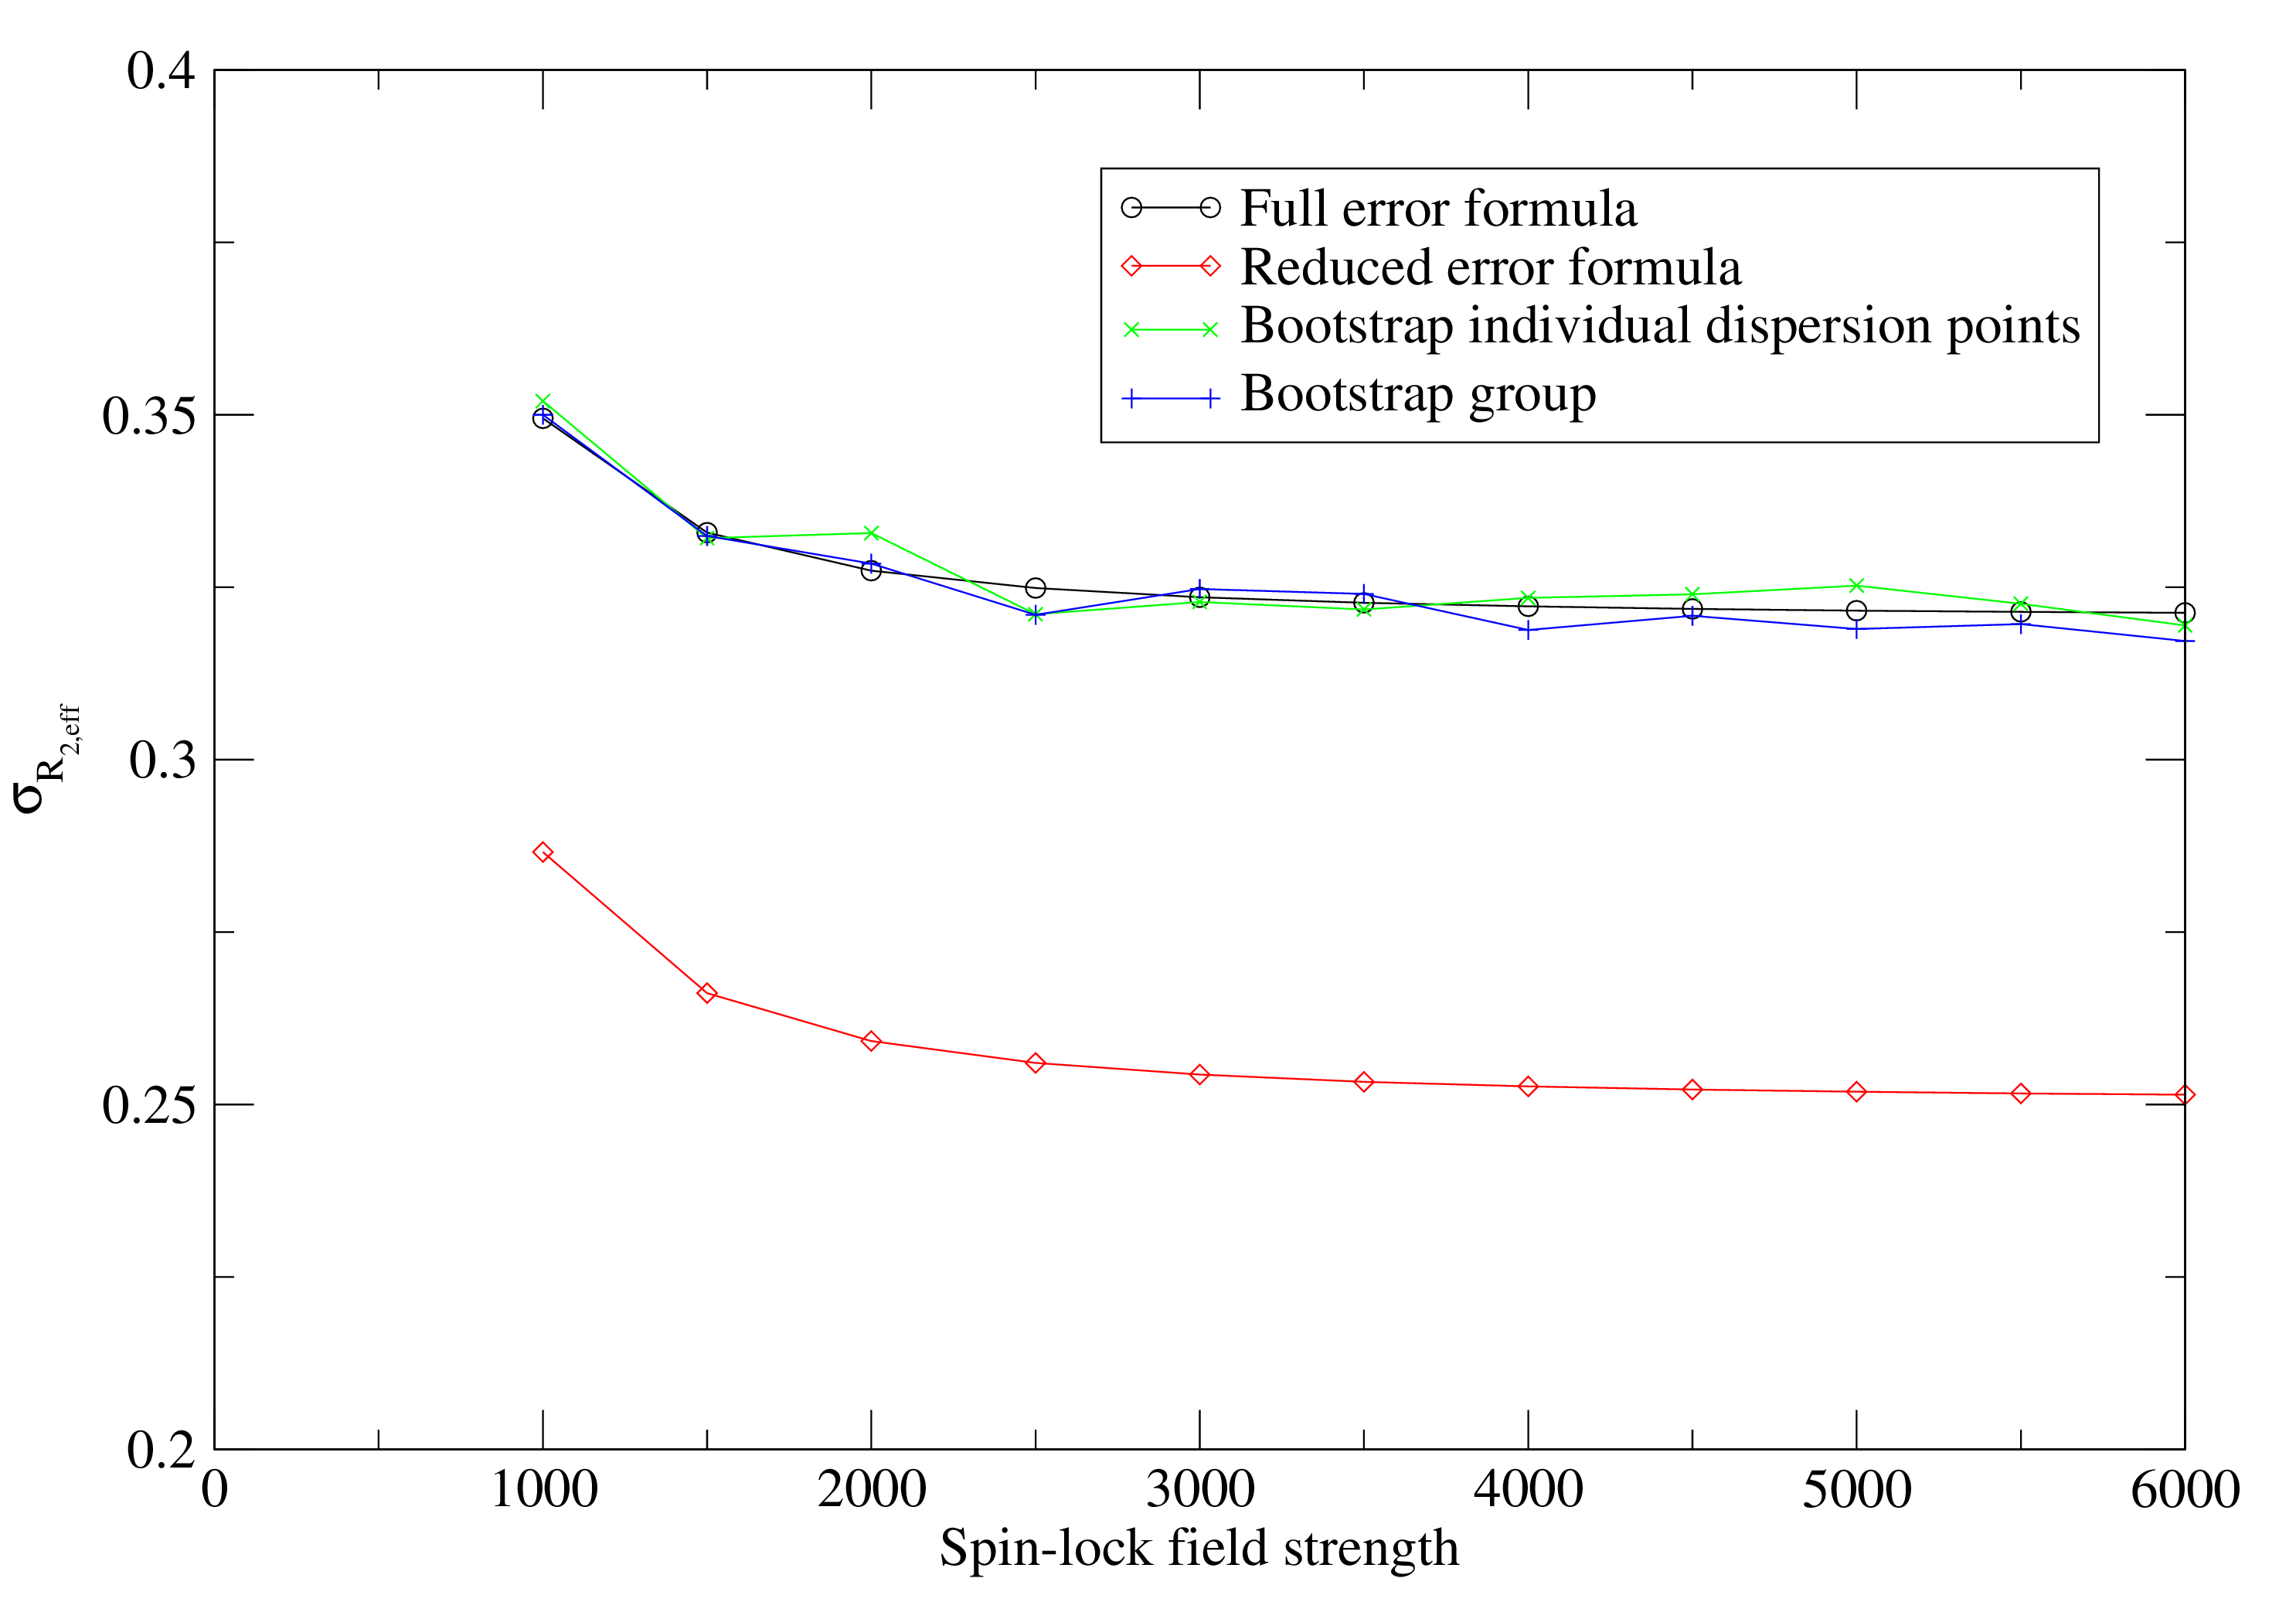
\includegraphics[
      width=0.9\textwidth,
      bb=14 14 728 512
    ]
    {graphics/analyses/dispersion/error_comparison}
  }
  \caption[Comparison of relaxation dispersion errors]{
    A demonstration of the inaccuracy of the error formula of Equation~\ref{eq: IT05 dispersion error} from \citet{IshimaTorchia05}.
    This plot was generated using the script \file{test\osus{}suite\ossep{}shared\osus{}data\ossep{}dispersion\ossep{}error\osus{}testing\ossep{}simulation.py}.
    The bootstrapping simulation involves randomising noise-free $I_0$ and $I_1$ values for each dispersion data point assuming Gaussian errors.
    The full error formula is from Equation~\ref{eq: dispersion error}, the reduced error formula is from Equation~\ref{eq: IT05 dispersion error}, the bootstrapping using individual dispersion points estimates the errors assuming different $I_0$ randomisations for each dispersion point and each simulation, and the bootstrapping group graph uses the same randomised $I_0$ value for all dispersion points for each simulation.
  }
  \label{fig: dispersion error comparison}
\end{figure*}


% Variable relaxation period experiments.
\subsubsection{Variable relaxation period experiments}

For the variable relaxation time period type experiments, the $\Rtwoeff$/$\Ronerho$ values are determined by fitting to the simple two parameter exponential as in a $\Rone$ or $\Rtwo$ analysis.
Both $\Rtwoeff$/$\Ronerho$ and the initial peak intensity $I_0$ are optimised using the minimise user function for each exponential curve separately.
Monte Carlo simulations are used to obtain the parameter errors.


% Links.
\subsubsection{Links}

More information about the R2eff model is available from:
\begin{itemize}
  \item the relax wiki at \url{http://wiki.nmr-relax.com/R2eff},
  \item the API documentation (for exponential curves) at \url{http://www.nmr-relax.com/api/3.2/specific\_analyses.relax\_disp.optimisation-module.html#back\_calc\_r2eff},
  \item the API documentation (for the 2-point fit) at \url{http://www.nmr-relax.com/api/3.2/lib.dispersion.two\_point-module.html#calc\_two\_point\_r2eff},
  \item the relaxation dispersion page of the relax website at \url{http://www.nmr-relax.com/analyses/relaxation\_dispersion.html#R2eff}.
\end{itemize}


% No Rex model.
%~~~~~~~~~~~~~~

\subsection{The model for no chemical exchange relaxation}
\label{sect: dispersion: No Rex model}
\index{relaxation dispersion!No Rex model|textbf}

This model is provided for model selection purposes.
In combination with frequentist methods, such as AIC\index{model selection!AIC}, or Bayesian methods\index{model selection!Bayesian} it can show if the presence of chemical exchange is statistically significant.
Optimisation is still required as one $\Rtwozero$ value per magnetic field strength will be fit to the measured data for each spin system.
If off-resonance CPMG or $\Ronerho$ data is being used, then one of the following equations will be fit:
\begin{subequations}
\begin{align}
    \Rtwoeff &= \Rone \cos^2\theta  +  \Rtwozero \sin^2\theta, \\
    \Ronerho &= \Rone \cos^2\theta  +  \Ronerhoprime \sin^2\theta.
\end{align}
\end{subequations}

The $\Rone$ value can either be fixed to loaded experimental values or optimised.
It is selected by setting the model to `No Rex'.

More information about the No Rex model is available from the:
\begin{itemize}
  \item the relax wiki at \url{http://wiki.nmr-relax.com/No\_Rex},
  \item the API documentation at \url{http://www.nmr-relax.com/api/3.2/target\_functions.relax\_disp.Dispersion-class.html#func\_NOREX},
  \item the relaxation dispersion page of the relax website at \url{http://www.nmr-relax.com/analyses/relaxation\_dispersion.html#No\_Rex}.
\end{itemize}



% The analytic CPMG models.
%%%%%%%%%%%%%%%%%%%%%%%%%%%

\section{The analytic CPMG models}
\label{sect: dispersion: analytic CPMG models}
\index{relaxation dispersion!Analytic CPMG model|textbf}

These are the analytic models designed for a single data type -- the single quantum CPMG-type experiment.


% LM63 model.
%~~~~~~~~~~~~

\subsection{The LM63 2-site fast exchange CPMG model}
\label{sect: dispersion: LM63 model}
\index{relaxation dispersion!LM63 model|textbf}

This is the original model for 2-site fast exchange for CPMG-type experiments.
It is selected by setting the model to `LM63', here named after \citet{LuzMeiboom63}.
The original $n$-site Equation~(7) from their paper can be written as
\begin{equation}
    \Rex = \left[ 1 - 2\tex g \cdot \tanh \left( 2\tex g \right)^{-1} \right] \cdot \tex \cdot \sum_{i=2}^n p_{\textrm{i}}\dw_{i},
\end{equation}

where $g$ is the pulse repetition rate defined as
\begin{equation}
    g = 2\nucpmg.
\end{equation}

It can be rearranged as
\begin{equation} \label{eq: Luz-Meiboom}
    \Rex = \sum_{i=2}^n \frac{\Phiexi}{\textrm{k}_{\textrm{i}}} \cdot \left( 1 - \frac{4\nucpmg}{\textrm{k}_{\textrm{i}}} \cdot \tanh \left( \frac{\textrm{k}_\textrm{i}}{4\nucpmg} \right) \right).
\end{equation}


The equation for the 2-site exchange process can be expressed as
\begin{equation}
    \Rtwoeff = \Rtwozero + \frac{\Phiex}{\kex} \cdot \left( 1 - \frac{4\nucpmg}{\kex} \cdot \tanh \left( \frac{\kex}{4\nucpmg} \right) \right).
\end{equation}

The reference for this equation is:
\begin{itemize}
  \item \bibentry{LuzMeiboom63}
\end{itemize}

More information about the LM63 model is available from:
\begin{itemize}
  \item the relax wiki at \url{http://wiki.nmr-relax.com/LM63},
  \item the API documentation at \url{http://www.nmr-relax.com/api/3.2/lib.dispersion.lm63-module.html},
  \item the relaxation dispersion page of the relax website at \url{http://www.nmr-relax.com/analyses/relaxation\_dispersion.html#LM63}.
\end{itemize}


% LM63 3-site model.
%~~~~~~~~~~~~~~~~~~~

\subsection{The LM63 3-site fast exchange CPMG model}
\label{sect: dispersion: LM63 3-site model}
\index{relaxation dispersion!LM63 3-site model|textbf}

This is the original \citet{LuzMeiboom63} model for 3-site fast exchange for CPMG-type experiments.
It is selected by setting the model to `LM63 3-site'.
Taking the original Equation~\ref{eq: Luz-Meiboom}, the equation for 3-site exchange is simply:
\begin{equation}
    \Rex = \sum_{i=2}^3 \frac{\Phiexi}{\textrm{k}_\textrm{i}} \cdot \left( 1 - \frac{4\nucpmg}{\textrm{k}_\textrm{i}} \cdot \tanh \left( \frac{\textrm{k}_\textrm{i}}{4\nucpmg} \right) \right) ,
\end{equation}

The reference for this equation is:
\begin{itemize}
  \item \bibentry{LuzMeiboom63}
\end{itemize}

This model is only provided as a demonstration and should not be used for a normal analysis.
Without data at multiple temperatures, a feature not currently supported within relax, that there are infinite lines of solutions and that the $\PhiexB$, $\PhiexC$, $\kB$ and $\kC$ parameters are all convoluted together.

This equation was made more practically relevant in the paper of \citet{OConnell09}.
This relies on the assumption that site~1 (or~A) has a much larger equilibrium population than the other sites ($\pA \gg \pB$ and $\pA \gg \pC$).
As stated, ``if the different values of ji are well-separated (by a factor of 3-10), then Eq.~3 reduces approximately to the sum of n~-~1 independent two-state processes for exchange between site~1 and the n~-~1 other sites''.
In this situation, the following relationships hold
\begin{subequations}
\begin{align}
    &\kB \approx \kexAB = \kAB + \kBA , \\
    &\kC \approx \kexAC = \kAC + \kCA ,
\end{align}
\end{subequations}

and
\begin{subequations}
\begin{align}
    &\PhiexB = \overline{\Phiex} \frac{\left(\kexAB\right)^2 \left( \overline{\kex} - \kexAC \right)}{\kex^2 \left( \kex - \kexAC \right)} , \label{eq: disp phiexB} \\
    &\PhiexC = \overline{\Phiex} \frac{\left(\kexAC\right)^2 \left( \overline{\kex} - \kexAB \right)}{\kex^2 \left( \kexAC - \kexAB \right)} , \label{eq: disp phiexC}
\end{align}
\end{subequations}

with
\begin{subequations}
\begin{align}
    &\overline{\PhiexB} \approx (\pA + \pC) \pB \dwAB^2 , \\
    &\overline{\PhiexC} \approx (\pA + \pB) \pC \dwAC^2 .
\end{align}
\end{subequations}

The parameter deconvolutions for this model can be performed after a relax analysis, if desired.

More information about the LM63 3-site model is available from:
\begin{itemize}
  \item the relax wiki at \url{http://wiki.nmr-relax.com/LM63\_3-site},
  \item the API documentation at \url{http://www.nmr-relax.com/api/3.2/lib.dispersion.lm63\_3site-module.html},
  \item the relaxation dispersion page of the relax website at \url{http://www.nmr-relax.com/analyses/relaxation\_dispersion.html#LM63\_3-site}.
\end{itemize}


% Full CR72 model.
%~~~~~~~~~~~~~~~~~

\subsection{The full CR72 2-site CPMG model}
\label{sect: dispersion: CR72 full model}
\index{relaxation dispersion!CR72 full model|textbf}

This is the model for 2-site exchange on most times scales (with the constraint that $\pA > \pB$), named after \citet{CarverRichards72}.
It is selected by setting the model to `CR72 full'.
The equation is
\begin{equation}
    \Rtwoeff = \frac{1}{2} \Big( \RtwozeroA + \RtwozeroB + \kex - 2\nucpmg\cosh^{-1} \big( D_+\cosh(\eta_+) - D_-\cos(\eta_-) \big) \Big) ,
\end{equation}

where
\begin{align}
    D_{\pm}    &= \frac{1}{2} \left( \pm1 + \frac{\Psi + 2\dw^2}{\sqrt{\Psi^2 + \zeta^2}} \right) , \\
    \eta_{\pm} &= 2^{\frac{-3}{2}}\frac{1}{\nucpmg} \left( \pm\Psi + \sqrt{\Psi^2 + \zeta^2} \right)^{\frac{1}{2}} , \\
    \Psi       &= \left( \RtwozeroA - \RtwozeroB - \pA\kex + \pB\kex \right)^2 - \dw^2 + 4\pA\pB\kex^2 , \\
    \zeta      &= 2\dw \left( \RtwozeroA - \RtwozeroB - \pA\kex + \pB\kex \right).
\end{align}

Note that these equations use the numerically simplified form derived in the appendix of \citet{Davis94}.

This model is not accurate when the motional process is very slow.
In that case, the `TSMFK01' model in Section~\ref{sect: dispersion: TSMFK01 model} on page~\pageref{sect: dispersion: TSMFK01 model} should be used instead.

The reference for this equation is:
\begin{itemize}
  \item \bibentry{CarverRichards72}
\end{itemize}

More information about the CR72 full model is available from:
\begin{itemize}
  \item the relax wiki at \url{http://wiki.nmr-relax.com/CR72\_full},
  \item the API documentation at \url{http://www.nmr-relax.com/api/3.2/lib.dispersion.cr72-module.html},
  \item the relaxation dispersion page of the relax website at \url{http://www.nmr-relax.com/analyses/relaxation\_dispersion.html#CR72\_full}.
\end{itemize}


% CR72 model.
%~~~~~~~~~~~~

\subsection{The reduced CR72 2-site CPMG model}
\label{sect: dispersion: CR72 model}
\index{relaxation dispersion!CR72 model|textbf}

This is the model for 2-site exchange on most times scales (with the constraint that $\pA > \pB$), named after \citet{CarverRichards72}.
It is selected by setting the model to `CR72'.
It is the same as the full CR72 model described above, but with the simplification that $\RtwozeroA = \RtwozeroB$.
This simplifies the equations to
\begin{equation}
    \Rtwoeff = \Rtwozero + \frac{\kex}{2} - \nucpmg\cosh^{-1} \big( D_+\cosh(\eta_+) - D_-\cos(\eta_-) \big) ,
\end{equation}

where $D_{\pm}$ and $\eta_{\pm}$ are unchanged and
\begin{align}
    \Psi  &= \kex^2 - \dw^2 , \\
    \zeta &= -2\dw (\pA\kex - \pB\kex) .
\end{align}

As mentioned in the `CR72 full' model section, this model is not accurate when the motional process is very slow.
In that case please use the `TSMFK01' model in Section~\ref{sect: dispersion: TSMFK01 model} on page~\pageref{sect: dispersion: TSMFK01 model} instead.

More information about the CR72 model is available from:
\begin{itemize}
  \item the relax wiki at \url{http://wiki.nmr-relax.com/CR72},
  \item the API documentation at \url{http://www.nmr-relax.com/api/3.2/lib.dispersion.cr72-module.html},
  \item the relaxation dispersion page of the relax website at \url{http://www.nmr-relax.com/analyses/relaxation\_dispersion.html#CR72}.
\end{itemize}


% IT99 model.
%~~~~~~~~~~~~

\subsection{The IT99 2-site CPMG model}
\label{sect: dispersion: IT99 model}
\index{relaxation dispersion!IT99 model|textbf}

This is the model for 2-site exchange on all times scales (with the constraint that $\pA \gg \pB$), named after \citet{IshimaTorchia99}.
It is selected by setting the model to `IT99'.
The equation is:
\begin{align}
    \Rex       &\simeq \frac{\Phiex\tex}{1 + \omega_a^2\tex^2} , \\
    \omega_a^2 &= \sqrt{\omega_{\textrm{1eff}}^4 + \pA^2\dw^4} , \\
    \Rtwoeff   &= \Rtwozero + \Rex .
\end{align}

The effective rotating frame field for a CPMG-type experiment is given by
\begin{equation}
    \omega_{\textrm{1eff}} = 4\sqrt{3}\nucpmg ,
\end{equation}

and hence
\begin{equation}
    \omega_{\textrm{1eff}}^4 = 2304\nucpmg^4 .
\end{equation}

The reference for this equation is:
\begin{itemize}
  \item \bibentry{IshimaTorchia99}
\end{itemize}

More information about the IT99 model is available from:
\begin{itemize}
  \item the relax wiki at \url{http://wiki.nmr-relax.com/IT99},
  \item the API documentation at \url{http://www.nmr-relax.com/api/3.2/lib.dispersion.it99-module.html},
  \item the relaxation dispersion page of the relax website at \url{http://www.nmr-relax.com/analyses/relaxation\_dispersion.html#IT99}.
\end{itemize}


% TSMFK01 model.
%~~~~~~~~~~~~~~~

\subsection{The TSMFK01 2-site CPMG model}
\label{sect: dispersion: TSMFK01 model}
\index{relaxation dispersion!TSMFK01 model|textbf}

This is the model for 2-site very-slow exchange model for time scales within range of microsecond to second time scale, where $\pA \gg \pB$, and named after \citet{Tollinger01}.
It is selected by setting the model to `TSMFK01'.
A particularly interesting feature of the dispersion curves is the damped oscillations, which occur at low CPMG field strengths, and is solely a function of the chemical shift difference between the two sites (i.e.\ independent of the rate of exchange).

The equation is:
\begin{equation}
    \Rtwoeff = \RtwozeroA + \kAB - \kAB \frac{\sin{(\dw \cdot \taucpmg )}}{\dw \cdot \taucpmg}
\end{equation}

The reference for this equation is:
\begin{itemize}
  \item \bibentry{Tollinger01}
\end{itemize}

More information about the TSMFK01 model is available from:
\begin{itemize}
  \item the relax wiki at \url{http://wiki.nmr-relax.com/TSMFK01},
  \item the API documentation at \url{http://www.nmr-relax.com/api/3.2/lib.dispersion.tsmfk01-module.html},
  \item the relaxation dispersion page of the relax website at \url{http://www.nmr-relax.com/analyses/relaxation\_dispersion.html#TSMFK01}.
\end{itemize}


% Full B14 model.
%~~~~~~~~~~~~~~~~~

\subsection{The full B14 2-site CPMG model}
\label{sect: dispersion: B14 full model}
\index{relaxation dispersion!B14 full model|textbf}

This is the model for 2-site exchange exact analytical derivation on all time scales (with the constraint that $\pA > \pB$), named after \citet{Baldwin2014}.
It is selected by setting the model to `B14 full'.
The equation is
\begin{subequations}
\begin{align}
  \Rtwoeff & = \frac{\RtwozeroA + \RtwozeroB + \kex}{2}-\frac{\ncyc}{\Trelax} \cosh{}^{-1}(\nu_{1c}) \nonumber \\
           & \qquad - \frac{1}{\Trelax}\ln{\left(\frac{1+y}{2} + \frac{1-y}{2\sqrt{\nu_{1c}^2-1}}(\nu_2 + 2\kAB p_D)\right)} , \\
    & = \RtwoeffCR - \frac{1}{\Trelax}\ln{\left(\frac{1+y}{2} + \frac{1-y}{2\sqrt{\nu_{1c}^2-1}}(\nu_2 + 2\kAB p_D)\right)} ,
\end{align}
\end{subequations}

where Appendix 1 in \citet{Baldwin2014} lists the recipe for the exact calculation of $\Rtwoeff$.
Note that the following definitions are different to those in the original publication, but match both the reference implementation and the relax implementation.
The definitions are functionally equivalent.
First establish the complex free precession eigenfrequency with
\begin{subequations}
\begin{align}
	\Delta \Rtwozero & = \RtwozeroA - \RtwozeroB , \\
	\alpha_- & = \Delta \Rtwozero + \kAB - \kBA , \\
	\zeta & = 2 \dw \alpha_- , \\
	\Psi & = \alpha_-^2 + 4 \kAB \kBA - \dw^2 , \\
	h_3 &= \frac{1}{\sqrt{2}}\sqrt{\Psi + \sqrt{\zeta^2 + \Psi^2} } , \\
    h_4 &= \frac{1}{\sqrt{2}}\sqrt{-\Psi + \sqrt{\zeta^2 + \Psi^2} } .
\end{align}
\end{subequations}

The ground state ensemble evolution frequency $f_{00}$ expressed in separated real and imaginary components in terms of definitions $\zeta$, $\Psi$, and $h_4$ is
\begin{equation}
	f_{00} = \frac{1}{2}\left(\RtwozeroA + \RtwozeroB + \kex\right) + \frac{\imath}{2}\left(\dw - h_4\right) .
\end{equation}

Define substitutions for `stay' and `swap' factors as
\begin{subequations}
\begin{align}
	N & = h_3 + \imath h_4 , \\
	NN^* & = h_3^2 + h_4^2 , \\
	F_0 & = \left(\dw^2 + h_3^2\right) / NN^* , \\
	F_2 & = \left(\dw^2 - h_4^2\right) / NN^* , \\
	F_1^b & = \left(\dw + h_4\right) \left(\dw - \imath h_3\right) / NN^* , \\
	F_1^{a+b} & = \left(2\dw^2 + \imath \zeta\right) / NN^* .
\end{align}
\end{subequations}

The weighting factors for frequencies $E_{0-2}$ emerging from a single CPMG block, $F_{0-2}$, are
\begin{subequations}
\begin{align}
	E_0 & =  2 \taucpmg \cdot h_3 , \\
	E_2 & =  2 \taucpmg \cdot  h_4 , \\
	E_1 & = (h_3 - \imath h_4) \cdot \taucpmg .
\end{align}
\end{subequations}

Here $\taucpmg = 1 / 4\nucpmg$.
The final result, with identities to assist efficient matrix exponentiation optimised for numerical calculation, is
\begin{subequations}
\begin{align}
	\nu_{1c} & = F_0  \cosh(E_0) - F_2 \cos(E_2) , \\
	\nu_{1s} & = F_0  \sinh(E_0) - \imath F_2 \sin(E_2), \\
	\nu_3 & = \sqrt{\nu_{1c}^2 - 1} , \\
	\nu_4 & = F_1^b (-\alpha_- - h_3) + \imath F_1^b (\dw - h_4) , \\
	\nu_5 & = \left(-\Delta \Rtwozero + \kex + \imath \dw\right) \nu_{1s} + 2 \left(\nu_4 + \kAB F_1^{a+b}\right) \sinh(E_1) , \\
    y & = \left( \frac{\nu_{1c} - \nu_3}{\nu_{1c} + \nu_3} \right) ^{\ncyc} , \\
	T & = \frac{1 + y}{2} + \frac{1 - y}{2} \frac{\nu_5}{\nu_3 N} , \\
	\RtwoeffCR & = \frac{\RtwozeroA + \RtwozeroB + \kex}{2} - \frac{\ncyc}{\Trelax} \, \arccosh\left(\Re(\nu_{1c})\right) , \\
	\Rtwoeff & = \RtwoeffCR - \frac{1}{\Trelax} \log\left(\Re(T)\right) .
\end{align}
\end{subequations}

The advantage of these equations is that you will always obtain the correct answer provided you have 2-site exchange, in-phase magnetisation and on-resonance pulses.

The term $p_D$ is based on product of the off diagonal elements in the CPMG propagator, see supplementary Section 3 \citep{Baldwin2014}.

It is interesting to consider the region of validity of the Carver and Richards result.
The two results are equal when the correction is zero, which is true when
\begin{equation}
    \sqrt{\nu_{1c}^2-1} \approx \nu_2 + 2 \kAB p_D .
\end{equation}

This occurs when $\kAB p_D$ tends to zero, and so $\nu_2 = \nu_3$.
Setting $\kAB p_D$ to zero amounts to neglecting magnetisation that starts on the ground state ensemble and end on the excited state ensemble and vice versa.
This will be a good approximation when $\pA \gg \pB$.
In practise, significant deviations from the Carver and Richards equation can be incurred if $\pB > 1$\%.
Incorporation of the correction term results in an improved description of the CPMG experiment over \citet{CarverRichards72}.

The reference for this equation is:
\begin{itemize}
  \item \bibentry{Baldwin2014}
\end{itemize}

More information about the B14 full model is available from:
\begin{itemize}
  \item the relax wiki at \url{http://wiki.nmr-relax.com/B14\_full},
  \item the API documentation at \url{http://www.nmr-relax.com/api/3.2/lib.dispersion.b14-module.html},
  \item the relaxation dispersion page of the relax website at \url{http://www.nmr-relax.com/analyses/relaxation\_dispersion.html#B14\_full}.
\end{itemize}


% B14 model.
%~~~~~~~~~~~~

\subsection{The reduced B14 2-site CPMG model}
\label{sect: dispersion: B14 model}
\index{relaxation dispersion!B14 model|textbf}

This is the model for 2-site exchange exact analytical derivation on all time scales (with the constraint that $\pA > \pB$), named after \citet{Baldwin2014}.
It is selected by setting the model to `B14'.
It is the same as the full B14 model described above, but with the simplification that $\RtwozeroA = \RtwozeroB$.

More information about the B14 model is available from:
\begin{itemize}
  \item the relax wiki at \url{http://wiki.nmr-relax.com/B14},
  \item the API documentation at \url{http://www.nmr-relax.com/api/3.2/lib.dispersion.b14-module.html},
  \item the relaxation dispersion page of the relax website at \url{http://www.nmr-relax.com/analyses/relaxation\_dispersion.html#B14}.
\end{itemize}


% The numeric CPMG models.
%%%%%%%%%%%%%%%%%%%%%%%%%%

\section{The numeric CPMG models}
\label{sect: dispersion: numeric CPMG models}
\index{relaxation dispersion!Numeric CPMG model|textbf}

These are the numeric models designed for a single data type -- the single quantum CPMG-type experiment.


% NS CPMG 2-site expanded model.
%~~~~~~~~~~~~~~~~~~~~~~~~~~~~~~~

\subsection{The NS 2-site expanded CPMG model}
\label{sect: dispersion: NS CPMG 2-site expanded model}
\index{relaxation dispersion!NS CPMG 2-site expanded model|textbf}

This is the numerical model for 2-site exchange expanded using Maple by Nikolai Skrynnikov.
It is selected by setting the model to `NS CPMG 2-site expanded'.
The simple constraint $\pA > \pB$ is used to halve the optimisation space, as both sides of the limit are mirror image spaces.

This model will give the same results as the other numerical solutions whereby $\RtwozeroA = \RtwozeroB$.
The following is the set of equations of the expansion used in relax.
It has been modified from the original for speed.
See the \module{lib\pysep{}dispersion\pysep{}ns\pyus{}cpmg\pyus{}2site\pyus{}expanded} module for more details including the original code.
Further simplifications can be found in the code.

\begin{latexonly}
\begin{subequations}
\renewcommand{\theequation}{\theparentequation .\arabic{equation}}
\begin{align}
      t_{3} &= \imath, \\
      t_{4} &= t_{3} \dw, \\
      t_{5} &= \kBA^2, \\
      t_{8} &= 2 t_{4} \kBA, \\
     t_{10} &= 2 \kBA \kAB, \\
     t_{11} &= \dw^2, \\
     t_{14} &= 2 t_{4} \kAB, \\
     t_{15} &= \kAB^2, \\
     t_{17} &= \sqrt{t_{5} - t_{8} + t_{10} - t_{11} + t_{14} + t_{15}}, \\
     t_{21} &= \exp \left(\frac{(-\kBA + t_{4} - \kAB + t_{17}) \taucpmg}{2} \right), \\
     t_{22} &= \frac{1}{t_{17}}, \\
     t_{28} &= \exp \left(\frac{(-\kBA + t_{4} - \kAB - t_{17}) \taucpmg}{2} \right), \\
     t_{31} &= t_{22} \kAB (t_{21} - t_{28}), \\
     t_{33} &= \sqrt{t_{5} + t_{8} + t_{10} - t_{11} - t_{14} + t_{15}}, \\
     t_{34} &= \kBA + t_{4} - \kAB + t_{33}, \\
     t_{37} &= \exp \left((-\kBA - t_{4} - \kAB + t_{33}) \taucpmg \right), \\
     t_{39} &= \frac{1}{t_{33}}, \\
     t_{41} &= \kBA + t_{4} - \kAB - t_{33}, \\
     t_{44} &= \exp \left((-\kBA - t_{4} - \kAB - t_{33}) \taucpmg \right), \\
     t_{47} &= \frac{t_{39}}{2} \left(t_{34} t_{37} - t_{41} t_{44} \right), \\
     t_{49} &= \kBA - t_{4} - \kAB - t_{17}, \\
     t_{51} &= t_{21} t_{49} t_{22}, \\
     t_{52} &= \kBA - t_{4} - \kAB + t_{17}, \\
     t_{54} &= t_{28} t_{52} t_{22}, \\
     t_{55} &= t_{54} - t_{51}, \\
     t_{60} &= \frac{1}{2} t_{39} \kAB \left(t_{37} - t_{44} \right), \\
     t_{62} &= t_{31} t_{47} + t_{55} t_{60}, \\
     t_{63} &= \frac{1}{\kAB}, \\
     t_{68} &= \frac{t_{63}}{2} \left(t_{49} t_{54} - t_{52} t_{51} \right), \\
     t_{69} &= \frac{t_{62} t_{68}}{2}, \\
     t_{72} &= t_{37} t_{41} t_{39}, \\
     t_{76} &= t_{44} t_{34} t_{39}, \\
     t_{78} &= \frac{t_{63}}{2} \left(t_{41} t_{76} - t_{34} t_{72} \right), \\
     t_{80} &= \frac{1}{2} (t_{76} - t_{72}), \\
     t_{82} &= \frac{1}{2} (t_{31} t_{78} + t_{55} t_{80}), \\
     t_{83} &= \frac{t_{82} t_{55}}{2}, \\
     t_{88} &= \frac{t_{22}}{2} \left(t_{52} t_{21} - t_{49} t_{28} \right), \\
     t_{91} &= t_{88} t_{47} + t_{68} t_{60}, \\
     t_{92} &= t_{91} t_{88}, \\
     t_{95} &= \frac{1}{2} (t_{88} t_{78} + t_{68} t_{80}), \\
     t_{96} &= t_{95} t_{31}, \\
     t_{97} &= t_{69} + t_{83}, \\
     t_{98} &= t_{97}^2, \\
     t_{99} &= t_{92} + t_{96}, \\
    t_{102} &= t_{99}^2, \\
    t_{108} &= t_{62} t_{88} + t_{82} t_{31}, \\
    t_{112} &= \sqrt{t_{98} - 2 t_{99} t_{97} + t_{102} + 2 (t_{91} t_{68} + t_{95} t_{55}) t_{108}}, \\
    t_{113} &= t_{97} - t_{99} - t_{112}, \\
    t_{115} &= n_{\textrm{CPMG}}, \\
    t_{116} &= \left( \frac{t_{97} + t_{99} + t_{112}}{2} \right)^{t_{115}}, \\
    t_{118} &= \frac{1}{t_{112}}, \\
    t_{120} &= t_{97} - t_{99} + t_{112}, \\
    t_{122} &= \left( \frac{t_{97} + t_{99} - t_{112}}{2} \right)^{t_{115}}, \\
    t_{127} &= \frac{1}{2 t_{108}}, \\
    t_{139} &= \frac{1}{2(\kAB + \kBA)} \Big[ (t_{120} t_{122} - t_{113} t_{116}) t_{118} \kBA \nonumber \\
            & \qquad \qquad                   + (t_{120} t_{122} - t_{116} t_{120}) t_{113} t_{118} t_{127} \kAB \Big].
\end{align}
\end{subequations}
\end{latexonly}

The relative peak intensities, magnetisation, and effective $\Rtwo$ relaxation rate are calculated as
\begin{subequations}
\begin{align}
    I_0 &= \pA, \\
    I_1 &= \Re(t_{139}) \exp(-\Trelax \Rtwozero), \\
    M_x &= I_1 / I_0, \\
    \Rtwoeff &= -\frac{1}{\Trelax} \cdot \ln \left( M_x \right). \label{eq: R2eff NS CPMG 2-site expanded}
\end{align}
\end{subequations}

In these equations $\taucpmg$ and $n_{\textrm{CPMG}}$ are numpy arrays and hence $t_{139}$ is also a numpy array.
This avoids a Python loop over the dispersion points until the very end of the calculation, required to populate the $\Rtwoeff$ data structure, resulting in very fast calculations.

The reference for this model is:
\begin{itemize}
  \item \bibentry{Tollinger01}
\end{itemize}

More information about the NS CPMG 2-site expanded model is available from:
\begin{itemize}
  \item the relax wiki at \url{http://wiki.nmr-relax.com/NS\_CPMG\_2-site\_expanded},
  \item the API documentation at \url{http://www.nmr-relax.com/api/3.2/lib.dispersion.ns\_cpmg\_2site\_expanded-module.html},
  \item the relaxation dispersion page of the relax website at \url{http://www.nmr-relax.com/analyses/relaxation\_dispersion.html#NS\_CPMG\_2-site\_expanded}.
\end{itemize}


% Full NS CPMG 2-site 3D model.
%~~~~~~~~~~~~~~~~~~~~~~~~~~~~~~

\subsection{The full NS 2-site 3D CPMG model}
\label{sect: dispersion: NS CPMG 2-site 3D full model}
\index{relaxation dispersion!NS CPMG 2-site 3D full model|textbf}

This is the numerical model for 2-site exchange using 3D magnetisation vectors.
It is selected by setting the model to `NS CPMG 2-site 3D full'.
The simple constraint $\pA > \pB$ is used to halve the optimisation space, as both sides of the limit are mirror image spaces.

More information about the NS CPMG 2-site 3D full model is available from:
\begin{itemize}
  \item the relax wiki at \url{http://wiki.nmr-relax.com/NS\_CPMG\_2-site\_3D\_full},
  \item the API documentation at \url{http://www.nmr-relax.com/api/3.2/lib.dispersion.ns\_cpmg\_2site\_3d-module.html},
  \item the relaxation dispersion page of the relax website at \url{http://www.nmr-relax.com/analyses/relaxation\_dispersion.html#NS\_CPMG\_2-site\_3D\_full}.
\end{itemize}


% Reduced NS CPMG 2-site 3D model.
%~~~~~~~~~~~~~~~~~~~~~~~~~~~~~~~~~

\subsection{The reduced NS 2-site 3D CPMG model}
\label{sect: dispersion: NS CPMG 2-site 3D model}
\index{relaxation dispersion!NS CPMG 2-site 3D model|textbf}

This is the numerical model for 2-site exchange using 3D magnetisation vectors, whereby the simplification $\RtwozeroA = \RtwozeroB$ is assumed.
It is selected by setting the model to `NS CPMG 2-site 3D'.
The simple constraint $\pA > \pB$ is used to halve the optimisation space, as both sides of the limit are mirror image spaces.

More information about the NS CPMG 2-site 3D model is available from:
\begin{itemize}
  \item the relax wiki at \url{http://wiki.nmr-relax.com/NS\_CPMG\_2-site\_3D},
  \item the API documentation at \url{http://www.nmr-relax.com/api/3.2/lib.dispersion.ns\_cpmg\_2site\_3d-module.html},
  \item the relaxation dispersion page of the relax website at \url{http://www.nmr-relax.com/analyses/relaxation\_dispersion.html#NS\_CPMG\_2-site\_3D}.
\end{itemize}


% Full NS CPMG 2-site star model.
%~~~~~~~~~~~~~~~~~~~~~~~~~~~~~~~~

\subsection{The full NS 2-site star CPMG model}
\label{sect: dispersion: NS CPMG 2-site star full model}
\index{relaxation dispersion!NS CPMG 2-site star full model|textbf}

This is the numerical model for 2-site exchange using complex conjugate matrices.
It is selected by setting the model to `NS CPMG 2-site star full'.
The simple constraint $\pA > \pB$ is used to halve the optimisation space, as both sides of the limit are mirror image spaces.

More information about the NS CPMG 2-site star full model is available from:
\begin{itemize}
  \item the relax wiki at \url{http://wiki.nmr-relax.com/NS\_CPMG\_2-site\_star\_full},
  \item the API documentation at \url{http://www.nmr-relax.com/api/3.2/lib.dispersion.ns\_cpmg\_2site\_star-module.html},
  \item the relaxation dispersion page of the relax website at \url{http://www.nmr-relax.com/analyses/relaxation\_dispersion.html#NS\_CPMG\_2-site\_star\_full}.
\end{itemize}


% Reduced NS CPMG 2-site star model.
%~~~~~~~~~~~~~~~~~~~~~~~~~~~~~~~~~~~

\subsection{The reduced NS 2-site star CPMG model}
\label{sect: dispersion: NS CPMG 2-site star model}
\index{relaxation dispersion!NS CPMG 2-site star model|textbf}

This is the numerical model for 2-site exchange using complex conjugate matrices, whereby the simplification $\RtwozeroA = \RtwozeroB$ is assumed.
It is selected by setting the model to `NS CPMG 2-site star'.
The simple constraint $\pA > \pB$ is used to halve the optimisation space, as both sides of the limit are mirror image spaces.

More information about the NS CPMG 2-site star model is available from:
\begin{itemize}
  \item the relax wiki at \url{http://wiki.nmr-relax.com/NS\_CPMG\_2-site\_star},
  \item the API documentation at \url{http://www.nmr-relax.com/api/3.2/lib.dispersion.ns\_cpmg\_2site\_star-module.html},
  \item the relaxation dispersion page of the relax website at \url{http://www.nmr-relax.com/analyses/relaxation\_dispersion.html#NS\_CPMG\_2-site\_star}.
\end{itemize}



% The analytic MMQ CPMG models.
%%%%%%%%%%%%%%%%%%%%%%%%%%%%%%%

\section{The analytic MMQ CPMG models}
\label{sect: dispersion: analytic MMQ CPMG models}
\index{relaxation dispersion!Analytic MMQ CPMG model|textbf}

These are the analytic models designed for handling combined proton-heteronuclear SQ, ZQ, DQ, and MQ CPMG-type experiments.
This data combination is labelled as multiple multiple quantum data or MMQ.


% MMQ CR72 model.
%~~~~~~~~~~~~~~~~

\subsection{The MMQ CR72 model}
\label{sect: dispersion: MMQ CR72 model}
\index{relaxation dispersion!MMQ CR72 model|textbf}

This is the analytic CR72 model for 2-site exchange on most times scales (Section~\ref{sect: dispersion: CR72 model} on page~\pageref{sect: dispersion: CR72 model}) extended for multiple types of multiple quantum data (MMQ) by \citet{Korzhnev04a}.
It is selected by setting the model to `MMQ CR72'.
The simple constraint $\pA > \pB$ is used to halve the optimisation space, as both sides of the limit are mirror image spaces.
The equation for the exchange process is 
\begin{equation}
    \Rtwoeff = \Re(\lambda_1) - \frac{1}{\Trelax}\ln(Q),
\end{equation}

where
\begin{align}
    \lambda_1  &= \RtwozeroMQ + \frac{\kex}{2} - \nucpmg\cosh^{-1} \big( D_+\cosh(\eta_+) - D_-\cos(\eta_-) \big), \\
    D_{\pm}    &= \frac{1}{2} \left( \pm1 + \frac{\Psi + 2\dw^2}{\sqrt{\Psi^2 + \zeta^2}} \right) , \\
    \eta_{\pm} &= 2^{\frac{2}{3}}\frac{1}{\nucpmg} \left( \pm\Psi + \sqrt{\Psi^2 + \zeta^2} \right)^{\frac{1}{2}} , \\
    \Psi       &= \left( \imath \dwH + \pA\kex - \pB\kex \right)^2 - \dw^2 + 4\pA\pB\kex^2 , \\
    \zeta      &= -2\dw \left( \imath \dwH + \pA\kex - \pB\kex \right),
\end{align}

and where
\begin{equation}
    Q = \Re \left( 1 - m_{D+}^2 + m_{D+} m_{Z+} - m_{Z+}^2 + \frac{m_{D+} + m_{Z+}}{2} \sqrt{\frac{\pB}{\pA}} \right),
\end{equation}

and
\begin{align}
    m_{D\pm} &= \pm \frac{\imath\kex\sqrt{\pA\pB}}{d_{\pm} z_\pm} \left( z_{\pm} + 2\dw \frac{\sin(z_{\pm}\delta)}{\sin((d_{\pm} + z_{\pm})\delta)} \right), \\
    m_{Z\mp} &= \pm \frac{\imath\kex\sqrt{\pA\pB}}{d_{\pm} z_\pm} \left( d_{\pm} - 2\dw \frac{\sin(d_{\pm}\delta)}{\sin((d_{\pm} + z_{\pm})\delta)} \right),
\end{align}

and
\begin{align}
    d_{\pm}    &= \left( \dwH + \dw \right) \pm \imath\kex, \\
    z_{\pm}    &= \left( \dwH - \dw \right) \pm \imath\kex.
\end{align}

The symbol $\delta$ is half of $\taucpmg$ or
\begin{equation}
    \delta = \frac{1}{4\nucpmg}.
\end{equation}

The references for this model are:
\begin{itemize}
  \item \bibentry{Korzhnev04a}
  \item \bibentry{Korzhnev04b}
  \item \bibentry{Korzhnev05b}
\end{itemize}

More information about the MMQ CR72 model is available from:
\begin{itemize}
  \item the relax wiki at \url{http://wiki.nmr-relax.com/MMQ\_CR72},
  \item the API documentation at \url{http://www.nmr-relax.com/api/3.2/lib.dispersion.mmq\_cr72-module.html},
  \item the relaxation dispersion page of the relax website at \url{http://www.nmr-relax.com/analyses/relaxation\_dispersion.html#MMQ\_CR72}.
\end{itemize}



% The numeric MMQ CPMG models.
%%%%%%%%%%%%%%%%%%%%%%%%%%%%%%

\section{The numeric MMQ CPMG models}
\label{sect: dispersion: numeric MMQ CPMG models}
\index{relaxation dispersion!Numeric MMQ CPMG model|textbf}

These are the numeric models designed for handling combined proton-heteronuclear SQ, ZQ, DQ, and MQ CPMG-type experiments.
This data combination is labelled as multiple multiple quantum data or MMQ.


% NS MMQ 2-site model.
%~~~~~~~~~~~~~~~~~~~~~

\subsection{The NS MMQ 2-site model}
\label{sect: dispersion: NS MMQ 2-site model}
\index{relaxation dispersion!NS MMQ 2-site model|textbf}

This is the numerical model for 2-site exchange for proton-heteronuclear SQ, ZQ, DQ and MQ CPMG data, as derived in \citep{Korzhnev04a,Korzhnev04b,Korzhnev05b}.
It is selected by setting the model to `NS MMQ 2-site'.
The simple constraint $\pA > \pB$ is used to halve the optimisation space, as both sides of the limit are mirror image spaces.
Different sets of equations are used for the different data types.


% The SQ, ZD and DQ equations.
\subsubsection{The SQ, ZD and DQ equations}

The basic evolution matrices for single, zero and double quantum CPMG-type data for this model are
\begin{equation}
    \Rtwoeff = - \frac{1}{\Trelax} \log \frac{\mathbf{M}_A(\Trelax)}{\mathbf{M}_A(0)},
\end{equation}

where $\mathbf{M}_A(0)$ is proportional to the vector $[\pA, \pB]^T$ and
\begin{equation}
    \mathbf{M}_A(\Trelax) = \left( \mathbf{A_{\pm}}\mathbf{A_\mp}\mathbf{A_\mp}\mathbf{A_{\pm}} \right)^n \mathbf{M}_A(0)
\end{equation}

The evolution matrix $\mathbf{A}$ is defined as
\begin{equation}
    \mathbf{A_{\pm}} = e^{\mathbf{a_{\pm}} \cdot \taucpmg},
\end{equation}

where
\begin{equation}
    \mathbf{a_{\pm}} = \begin{pmatrix}
                       -\kAB -\RtwozeroA & \kBA \\
                       \kAB  & -\kBA \pm\imath\dw - \RtwozeroB
                     \end{pmatrix}.
\end{equation}

For different data types $\dw$ is defined as:  $\dw$ ($^{15}$N SQ-type data);  $\dwH$ ($^1$H SQ-type data); $\dwH - \dw$ (ZQ-type data); and $\dwH + \dw$ (DQ-type data).



% The MQ equations.
\subsubsection{The MQ equations}

The equation for the exchange process for multiple quantum CPMG-type data is 
\begin{equation}
    \Rtwoeff = - \frac{1}{T}
                 \log \left\{ Re \left[ \frac{0.5}{\pA}
                     \begin{pmatrix}1&0\end{pmatrix} \cdot \left( \mathbf{AB} + \mathbf{CD} \right) \cdot \begin{pmatrix}\pA\\\pB\end{pmatrix}
                 \right] \right\},
\end{equation}

where $T$ is the constant time interval, and the matrices $\mathbf{A}$, $\mathbf{B}$, $\mathbf{C}$, and $\mathbf{D}$ are dually defined.
When $n$ is even, they are defined as 
\begin{subequations}
\begin{align}
    \mathbf{A} &= \left( \mathbf{M_1} \mathbf{M_2} \mathbf{M_2} \mathbf{M_1} \right)^{\frac{n}{2}}, \\
    \mathbf{B} &= \left( \mathbf{M_2}^* \mathbf{M_1}^* \mathbf{M_1}^* \mathbf{M_2}^* \right)^{\frac{n}{2}}, \\
    \mathbf{C} &= \left( \mathbf{M_2} \mathbf{M_1} \mathbf{M_1} \mathbf{M_2} \right)^{\frac{n}{2}}, \\
    \mathbf{D} &= \left( \mathbf{M_1}^* \mathbf{M_2}^* \mathbf{M_2}^* \mathbf{M_1}^* \right)^{\frac{n}{2}}.
\end{align}
\end{subequations}

When $n$ is odd, they are defined as
\begin{subequations}
\begin{align}
    \mathbf{A} &= \left( \mathbf{M_1} \mathbf{M_2} \mathbf{M_2} \mathbf{M_1} \right)^{\frac{n-1}{2}} \mathbf{M_1} \mathbf{M_2}, \\
    \mathbf{B} &= \left( \mathbf{M_1}^* \mathbf{M_2}^* \mathbf{M_2}^* \mathbf{M_1}^* \right)^{\frac{n-1}{2}} \mathbf{M_1}^* \mathbf{M_2}^*, \\
    \mathbf{C} &= \left( \mathbf{M_2} \mathbf{M_1} \mathbf{M_1} \mathbf{M_2} \right)^{\frac{n-1}{2}} \mathbf{M_2} \mathbf{M_1}, \\
    \mathbf{D} &= \left( \mathbf{M_2}^* \mathbf{M_1}^* \mathbf{M_1}^* \mathbf{M_2}^* \right)^{\frac{n-1}{2}} \mathbf{M_2}^* \mathbf{M_1}^*.
\end{align}
\end{subequations}

When $n$ is zero, to avoid matrix powers of zero they are defined as
\begin{subequations}
\begin{align}
    \mathbf{A} &= \mathbf{M_1} \mathbf{M_2}, \\
    \mathbf{B} &= \mathbf{M_1}^* \mathbf{M_2}^*, \\
    \mathbf{C} &= \mathbf{M_2} \mathbf{M_1}, \\
    \mathbf{D} &= \mathbf{M_2}^* \mathbf{M_1}^*.
\end{align}
\end{subequations}

The $\mathbf{M}$ matrices are defined as:
\begin{equation}
    \mathbf{M_j} = \exp(\mathbf{m_j}\delta),
\end{equation}

where $2\delta$ is the spacing between successive 180$^\circ$ pulses and where
The references for this model are:
\begin{subequations}
\begin{align}
    \mathbf{m_1} &= \begin{pmatrix}
                        -\pB\kex - \RtwoDQA & \pA\kex \\
                        \pB\kex & - \pA\kex -\imath(\dwH + \dw) - \RtwoDQB 
                    \end{pmatrix}, \\
    \mathbf{m_2} &=  \begin{pmatrix}
                        -\pB\kex - \RtwoZQA & \pA\kex \\
                        \pB\kex & - \pA\kex -\imath(\dwH - \dw) - \RtwoZQB 
                    \end{pmatrix}.
\end{align}
\end{subequations}

For the model it is assumed that $\RtwoDQA = \RtwoZQA = \RtwozeroA$ and $\RtwoDQB = \RtwoZQB = \RtwozeroB$.
The references for this model are:
\begin{itemize}
  \item \bibentry{Korzhnev04a}
  \item \bibentry{Korzhnev04b}
  \item \bibentry{Korzhnev05b}
\end{itemize}

More information about the NS MMQ 2-site model is available from:
\begin{itemize}
  \item the relax wiki at \url{http://wiki.nmr-relax.com/NS\_MMQ\_2-site},
  \item the API documentation at \url{http://www.nmr-relax.com/api/3.2/lib.dispersion.ns\_mmq\_2site-module.html},
  \item the relaxation dispersion page of the relax website at \url{http://www.nmr-relax.com/analyses/relaxation\_dispersion.html#NS\_MMQ\_2-site}.
\end{itemize}


% NS MMQ 3-site linear model.
%~~~~~~~~~~~~~~~~~~~~~~~~~~~~

\subsection{The NS MMQ 3-site linear model}
\label{sect: dispersion: NS MMQ 3-site linear model}
\index{relaxation dispersion!NS MMQ 3-site linear model|textbf}

This is the numerical model for 3-site exchange for proton-heteronuclear SQ, ZQ, DQ and MQ CPMG data, as derived in \citep{Korzhnev04a,Korzhnev04b,Korzhnev05b}.
As this model is linear, the assumption that $\kAC$~= $\kCA$~= 0 has been made.
To simplify the optimisation space for the model, the assumption $\RtwozeroA$~= $\RtwozeroB$~= $\RtwozeroC$~= $\Rtwozero$ has also been made.


% The SQ, ZD and DQ equations.
\subsubsection{The SQ, ZD and DQ equations}

The basic evolution matrices for single, zero and double quantum CPMG-type data for this model are
\begin{equation}
    \mathbf{A_{\pm}} = e^{\mathbf{a_{\pm}} \cdot \taucpmg},
\end{equation}

where
\begin{align}
    \mathbf{a_{\pm}} &= \begin{pmatrix}
                          -\kAB & \kBA                          & 0    \\
                          \kAB  & -\kBA -\kBC \pm\imath\dwAB    & \kCB \\
                          0     & \kBC                          & -\kCB \pm\imath\dwAC
                        \end{pmatrix}  \nonumber \\
                     &\qquad - \begin{pmatrix}
                                 \RtwozeroA & 0          & 0    \\
                                 0          & \RtwozeroB & 0    \\
                                 0          & 0          & \RtwozeroC
                               \end{pmatrix}.
\end{align}


% The MQ equations.
\subsubsection{The MQ equations}

The formulae for multiple quantum CPMG-type data are the same as for the `NS MMQ 2-site' model except for the $\Rtwoeff$ calculation and the $\mathbf{m_j}$ matrices.
The rate is calculated as
\begin{equation}
    \Rtwoeff = - \frac{1}{T}
                 \log \left\{ Re \left[ \frac{0.5}{\pA}
                     \begin{pmatrix}1&0&0\end{pmatrix} \cdot \left( \mathbf{AB} + \mathbf{CD} \right) \cdot \begin{pmatrix}\pA\\\pB\\\pC\end{pmatrix}
                 \right] \right\}.
\end{equation}

The $\mathbf{m_j}$ matrices are
\begin{subequations}
\begin{align}
    \mathbf{m_1} &= \begin{pmatrix}
                        -\kAB   & \kBA                                  & 0    \\
                        \kAB    & -\kBA -\kBC -\imath(\dwHAB + \dwAB)   & \kCB \\
                        0       & \kBC                                  & - \kCB  -\imath(\dwHAC + \dwAC)
                    \end{pmatrix}  \nonumber \\
                 &\qquad - \begin{pmatrix}
                               \RtwozeroA & 0          & 0    \\
                               0          & \RtwozeroB & 0    \\
                               0          & 0          & \RtwozeroC
                           \end{pmatrix}, \\
    \mathbf{m_2} &= \begin{pmatrix}
                        -\kAB   & \kBA                                  & 0    \\
                        \kAB    & -\kBA -\kBC -\imath(\dwHAB - \dwAB)   & \kCB \\
                        0       & \kBC                                  & -\kCB -\imath(\dwHAC - \dwAC)
                    \end{pmatrix}  \nonumber \\
                 &\qquad - \begin{pmatrix}
                               \RtwozeroA & 0          & 0    \\
                               0          & \RtwozeroB & 0    \\
                               0          & 0          & \RtwozeroC
                           \end{pmatrix}.
\end{align}
\end{subequations}

For the model, the assumption $\RtwozeroA = \RtwozeroB = \RtwozeroC = \Rtwozero$ is made.

More information about the NS MMQ 3-site linear model is available from:
\begin{itemize}
  \item the relax wiki at \url{http://wiki.nmr-relax.com/NS\_MMQ\_3-site\_linear},
  \item the API documentation at \url{http://www.nmr-relax.com/api/3.2/lib.dispersion.ns\_mmq\_3site-module.html},
  \item the relaxation dispersion page of the relax website at \url{http://www.nmr-relax.com/analyses/relaxation\_dispersion.html#NS\_MMQ\_3-site\_linear}.
\end{itemize}


% NS MMQ 3-site model.
%~~~~~~~~~~~~~~~~~~~~~

\subsection{The NS MMQ 3-site model}
\label{sect: dispersion: NS MMQ 3-site model}
\index{relaxation dispersion!NS MMQ 3-site model|textbf}

This is the numerical model for 3-site exchange for proton-heteronuclear SQ, ZQ, DQ and MQ CPMG data, as derived in \citep{Korzhnev04a,Korzhnev04b,Korzhnev05b}.
However it has been extended to allow the $A \leftrightarrow C$ transition.
To simplify the optimisation space for the model as in the `NS MMQ 3-site linear' model, the assumption $\RtwozeroA$~= $\RtwozeroB$~= $\RtwozeroC$~= $\Rtwozero$ has been made.


% The SQ, ZD and DQ equations.
\subsubsection{The SQ, ZD and DQ equations}

The basic evolution matrices for single, zero and double quantum CPMG-type data for this model are
\begin{equation}
    \mathbf{A_{\pm}} = e^{\mathbf{a_{\pm}} \cdot \taucpmg},
\end{equation}

where
\begin{align}
    \mathbf{a_{\pm}} &= \begin{pmatrix}
                          -\kAB -\kAC & \kBA                          & \kCA \\
                          \kAB        & -\kBA -\kBC \pm\imath\dwAB    & \kCB \\
                          \kAC        & \kBC                          & -\kCB -\kCA \pm\imath\dwAC
                        \end{pmatrix}  \nonumber \\
                     &\qquad - \begin{pmatrix}
                                 \RtwozeroA & 0          & 0    \\
                                 0          & \RtwozeroB & 0    \\
                                 0          & 0          & \RtwozeroC
                               \end{pmatrix}.
\end{align}


% The MQ equations.
\subsubsection{The MQ equations}

The $\mathbf{m_j}$ matrices for this model are
\begin{subequations}
\begin{align}
    \mathbf{m_1} &= \begin{pmatrix}
                        -\kAB -\kAC & \kBA                                  & \kCA \\
                        \kAB        & -\kBA -\kBC -\imath(\dwHAB + \dwAB)   & \kCB \\
                        \kAC        & \kBC                                  & -\kCB -\kCA -\imath(\dwHAC + \dwAC)
                    \end{pmatrix}  \nonumber \\
                 &\qquad - \begin{pmatrix}
                               \RtwozeroA & 0          & 0    \\
                               0          & \RtwozeroB & 0    \\
                               0          & 0          & \RtwozeroC
                           \end{pmatrix}, \\
    \mathbf{m_2} &= \begin{pmatrix}
                        -\kAB -\kAC & \kBA                                  & \kCA \\
                        \kAB        & -\kBA -\kBC -\imath(\dwHAB - \dwAB)   & \kCB \\
                        \kAC        & \kBC                                  & -\kCB -\kCA -\imath(\dwHAC - \dwAC)
                    \end{pmatrix}  \nonumber \\
                 &\qquad - \begin{pmatrix}
                               \RtwozeroA & 0          & 0    \\
                               0          & \RtwozeroB & 0    \\
                               0          & 0          & \RtwozeroC
                           \end{pmatrix}.
\end{align}
\end{subequations}

More information about the NS MMQ 3-site model is available from:
\begin{itemize}
  \item the relax wiki at \url{http://wiki.nmr-relax.com/NS\_MMQ\_3-site},
  \item the API documentation at \url{http://www.nmr-relax.com/api/3.2/lib.dispersion.ns\_mmq\_3site-module.html},
  \item the relaxation dispersion page of the relax website at \url{http://www.nmr-relax.com/analyses/relaxation\_dispersion.html#NS\_MMQ\_3-site}.
\end{itemize}



% The analytic R1rho models.
%%%%%%%%%%%%%%%%%%%%%%%%%%%

\section{The analytic $\Ronerho$ models}
\label{sect: dispersion: analytic R1rho models}
\index{relaxation dispersion!Analytic R1rho model|textbf}

These are the analytic models designed for $\Ronerho$-type experiments.


% M61 model.
%~~~~~~~~~~~

\subsection{The M61 2-site fast exchange $\Ronerho$ model}
\label{sect: dispersion: M61 model}
\index{relaxation dispersion!M61 model|textbf}

This is the model for 2-site fast exchange for on-resonance $\Ronerho$-type data.
It is selected by setting the model to `M61', here named after \citet{Meiboom61}.
The equation for the exchange process is
\begin{equation}
    \Ronerho = \Ronerhoprime + \frac{\Phiex\kex}{\kex^2 + \omegae^2}.
\end{equation}

The reference for this equation is:
\begin{itemize}
  \item \bibentry{Meiboom61}
\end{itemize}

More information about the M61 model is available from:
\begin{itemize}
  \item the relax wiki at \url{http://wiki.nmr-relax.com/M61},
  \item the API documentation at \url{http://www.nmr-relax.com/api/3.2/lib.dispersion.m61-module.html},
  \item the relaxation dispersion page of the relax website at \url{http://www.nmr-relax.com/analyses/relaxation\_dispersion.html#M61}.
\end{itemize}


% M61 skew model.
%~~~~~~~~~~~~~~~~

\subsection{The M61 skew 2-site fast exchange $\Ronerho$ model}
\label{sect: dispersion: M61 skew model}
\index{relaxation dispersion!M61 skew model|textbf}

This is the second model for 2-site fast exchange for on-resonance $\Ronerho$-type data from \citet{Meiboom61}.
It is selected by setting the model to `M61 skew'.
The equation for the exchange process is
\begin{equation}
    \Ronerho = \Ronerhoprime + \frac{\pA^2\pB\dw^2\kex}{\kex^2 + \pA^2\dw^2 + \omegaone^2}.
\end{equation}

Care must be taken as this model appears to have infinite lines of solutions -- $\pA$ and $\dw$ are convoluted.
Hence this model is disabled in the dispersion auto-analysis.

More information about the M61 skew model is available from:
\begin{itemize}
  \item the relax wiki at \url{http://wiki.nmr-relax.com/M61\_skew},
  \item the API documentation at \url{http://www.nmr-relax.com/api/3.2/lib.dispersion.m61b-module.html},
  \item the relaxation dispersion page of the relax website at \url{http://www.nmr-relax.com/analyses/relaxation\_dispersion.html#M61\_skew}.
\end{itemize}


% DPL94 model.
%~~~~~~~~~~~~~

\subsection{The DPL94 2-site fast exchange $\Ronerho$ model}
\label{sect: dispersion: DPL94 model}
\index{relaxation dispersion!DPL94 model|textbf}

This is the model for 2-site fast exchange for $\Ronerho$-type data.
It is selected by setting the model to `DPL94', here named after \citet{Davis94}.
It extends the \citet{Meiboom61} model to off-resonance data.
The model collapses to the M61 model for on-resonance data.
The equation for the exchange process is
\begin{equation}
    \Ronerho = \Rone \cos^2\theta  +  \left( \Ronerhoprime + \frac{\Phiex\kex}{\kex^2 + \omegae^2} \right) \sin^2\theta,
\end{equation}

where $\theta$ is the rotating frame tilt angle.
The reference for this equation is:
\begin{itemize}
  \item \bibentry{Davis94}
\end{itemize}

More information about the DPL94 model is available from:
\begin{itemize}
  \item the relax wiki at \url{http://wiki.nmr-relax.com/DPL94},
  \item the API documentation at \url{http://www.nmr-relax.com/api/3.2/lib.dispersion.dpl94-module.html},
  \item the relaxation dispersion page of the relax website at \url{http://www.nmr-relax.com/analyses/relaxation\_dispersion.html#DPL94}.
\end{itemize}


% TP02 model.
%~~~~~~~~~~~~

\subsection{The TP02 2-site exchange $\Ronerho$ model}
\label{sect: dispersion: TP02 model}
\index{relaxation dispersion!TP02 model|textbf}

This is the model for 2-site exchange for off-resonance $\Ronerho$-type data from \citet{TrottPalmer02}.
It is selected by setting the model to `TP02'.
The equation for the exchange process is
\begin{equation}
    \Ronerho = \Rone\cos^2\theta + \Ronerhoprime\sin^2\theta + \frac{\sin^2\theta\pA\pB\dw^2\kex}{\omega_\textrm{Aeff}^2\omega_\textrm{Beff}^2/\omega_\textrm{eff}^2 + \kex^2},
\end{equation}

in which
\begin{subequations}
\begin{align}
    \delta_A &= \omegaA - \omegarf, \label{eq: deltaA}\\
    \delta_B &= \omegaB - \omegarf, \label{eq: deltaB} \\
    \aveomega &= \pA\omegaA + \pB\omegaB, \\
    \aveoffset &= \aveomega - \omegarf, \\
    \omega_\textrm{Aeff}^2 &= \omegaone^2 + \delta_A^2, \\
    \omega_\textrm{Beff}^2 &= \omegaone^2 + \delta_B^2, \\
    \omega_\textrm{eff}^2 &= \omegaone^2 + \aveoffset^2, \\
    \theta &= \arctan \left( \frac{\omegaone}{\aveoffset} \right).
\end{align}
\end{subequations}

The equation is accurate only when populations are highly skewed with $\pA \gg \pB$.
And it is valid only for exchange processes which are not fast.
Note that this model has been superseded by the `TAP03' and `MP05' models.
The reference for this equation is:
\begin{itemize}
  \item \bibentry{TrottPalmer02}
\end{itemize}

More information about the TP02 model is available from:
\begin{itemize}
  \item the relax wiki at \url{http://wiki.nmr-relax.com/TP02},
  \item the API documentation at \url{http://www.nmr-relax.com/api/3.2/lib.dispersion.tp02-module.html},
  \item the relaxation dispersion page of the relax website at \url{http://www.nmr-relax.com/analyses/relaxation\_dispersion.html#TP02}.
\end{itemize}


% TAP03 model.
%~~~~~~~~~~~~

\subsection{The TAP03 2-site exchange $\Ronerho$ model}
\label{sect: dispersion: TAP03 model}
\index{relaxation dispersion!TAP03 model|textbf}

This is the model for 2-site exchange for off-resonance $\Ronerho$-type data from \citet{Trott03}.
It is selected by setting the model to `TAP03'.
The equation for the exchange process is
\begin{align}
    \Ronerho = & \Rone\cos^2\theta + \Ronerhoprime\sin^2\theta \nonumber \\
               & + \left( \frac{1}{\gamma} \right) 
                        \frac{\sin^2\hat\theta\pA\pB\dw^2\kex}{\hat\omega_\textrm{Aeff}^2\hat\omega_\textrm{Beff}^2/\hat\omega_\textrm{eff}^2 + \kex^2 - 2\sin^2\hat\theta\pA\pB\dw^2 + (1 - \gamma)\omegaone^2},
\end{align}

in which, in addition to those parameters defined above for the `TP02' model,
\begin{subequations}
\begin{align}
    \sigma &= \pB\delta_A + \pA\delta_B, \\
    \gamma &= 1 - \pA\pB\dw^2 \frac{\sigma^2 - \kex^2 + \omegaone^2}{\left( \sigma^2 + \kex^2 + \omegaone^2 \right)^2}, \\
    \hat\omega_\textrm{Aeff}^2 &= \gamma\omegaone^2 + \delta_A^2, \\
    \hat\omega_\textrm{Beff}^2 &= \gamma\omegaone^2 + \delta_B^2, \\
    \hat\omega_\textrm{eff}^2 &= \gamma\omegaone^2 + \aveoffset^2, \\
    \hat\theta &= \arctan \left( \frac{\sqrt{\gamma}\omegaone}{\aveoffset} \right).
\end{align}
\end{subequations}

The equation is accurate when populations are less skewed than the `TP02' model ($\pA \gg \pB$).
Note that this model, as with the `TP02' model, has been superseded by the `MP05' model in the next section.
The reference for this equation is:
\begin{itemize}
  \item \bibentry{Trott03}
\end{itemize}

More information about the TAP03 model is available from:
\begin{itemize}
  \item the relax wiki at \url{http://wiki.nmr-relax.com/TAP03},
  \item the API documentation at \url{http://www.nmr-relax.com/api/3.2/lib.dispersion.tap03-module.html},
  \item the relaxation dispersion page of the relax website at \url{http://www.nmr-relax.com/analyses/relaxation\_dispersion.html#TAP03}.
\end{itemize}


% MP05 model.
%~~~~~~~~~~~~

\subsection{The MP05 2-site exchange $\Ronerho$ model}
\label{sect: dispersion: MP05 model}
\index{relaxation dispersion!MP05 model|textbf}

This is the model for 2-site exchange for off-resonance $\Ronerho$-type data for all time scales from \citet{MiloushevPalmer05}.
It is selected by setting the model to `MP05'.
The equation for the exchange process is
\begin{align}
    \Ronerho = & \Rone\cos^2\theta + \Ronerhoprime\sin^2\theta \nonumber \\
               & + \frac{\sin^2\theta\pA\pB\dw^2\kex}{\omega_\textrm{Aeff}^2\omega_\textrm{Beff}^2/\omega_\textrm{eff}^2 + \kex^2 - \sin^2\theta\pA\pB\dw^2 \left(
                        1 + \frac{2\kex^2 \left( \pA\omega_\textrm{Aeff}^2 + \pB\omega_\textrm{Beff}^2 \right)}{\omega_\textrm{Aeff}^2\omega_\textrm{Beff}^2 + \omega_\textrm{eff}^2\kex^2}
                    \right)},
\end{align}

in which the parameters are defined as in the `TP02' model above.
This model supersedes both the `TP02' and `TAP03' models.
The reference for this equation is:
\begin{itemize}
  \item \bibentry{MiloushevPalmer05}
\end{itemize}

More information about the MP05 model is available from:
\begin{itemize}
  \item the relax wiki at \url{http://wiki.nmr-relax.com/MP05},
  \item the API documentation at \url{http://www.nmr-relax.com/api/3.2/lib.dispersion.mp05-module.html},
  \item the relaxation dispersion page of the relax website at \url{http://www.nmr-relax.com/analyses/relaxation\_dispersion.html#MP05}.
\end{itemize}



% The numeric R1rho models.
%%%%%%%%%%%%%%%%%%%%%%%%%%%

\section{The numeric $\Ronerho$ models}
\label{sect: dispersion: numeric R1rho models}
\index{relaxation dispersion!Numeric R1rho model|textbf}

These are the numeric models designed for $\Ronerho$-type experiments.


% NS R1rho 2-site model.
%~~~~~~~~~~~~~~~~~~~~~~~

\subsection{The NS 2-site $\Ronerho$ model}
\label{sect: dispersion: NS R1rho 2-site model}
\index{relaxation dispersion!NS R1rho 2-site model|textbf}

This is the numerical model for 2-site exchange using 3D magnetisation vectors.
It is selected by setting the model to `NS R1rho 2-site'.
The simple constraint $\pA > \pB$ is used to halve the optimisation space, as both sides of the limit are mirror image spaces.

For this model, the equations from \citet{Korzhnev05a} have been used.
The $\Ronerho$ value for state A magnetisation is defined as
\begin{equation}
    \Ronerho = - \frac{1}{\Trelax}  \cdot \ln \left( M_0^T \cdot e^{R \cdot \Trelax} \cdot M_0 \right),
\end{equation}

where
\begin{align}
    M_0    &= \begin{pmatrix} \sin{\theta} \\ 0 \\ \cos{\theta} \\ 0 \\ 0 \\ 0  \end{pmatrix}, \\
    \theta &= \arctan \left( \frac{\omegaone}{\offsetA} \right).
\end{align}

The relaxation evolution matrix is defined as
\begin{equation}
    R = \begin{pmatrix}
          -\Ronerhoprime-\kAB & -\delta_A           & 0           & \kBA                & 0                   & 0 \\
          \delta_A            & -\Ronerhoprime-\kAB & -\omegaone  & 0                   & \kBA                & 0 \\
          0                   & \omegaone           & -\Rone-\kAB & 0                   & 0                   & \kBA \\
          \kAB                & 0                   & 0           & -\Ronerhoprime-\kBA & -\delta_B           & 0 \\
          0                   & \kAB                & 0           & \delta_B            & -\Ronerhoprime-\kBA & -\omegaone \\
          0                   & 0                   & \kAB        & 0                   & \omegaone           & -\Rone-\kBA \\
        \end{pmatrix},
\end{equation}

where $\delta_{A,B}$ is defined in Equations~\ref{eq: deltaA} and~\ref{eq: deltaB}.

More information about the NS R1rho 2-site model is available from:
\begin{itemize}
  \item the relax wiki at \url{http://wiki.nmr-relax.com/NS\_R1rho\_2-site},
  \item the API documentation at \url{http://www.nmr-relax.com/api/3.2/lib.dispersion.ns\_r1rho\_2site-module.html},
  \item the relaxation dispersion page of the relax website at \url{http://www.nmr-relax.com/analyses/relaxation\_dispersion.html#NS\_R1rho\_2-site}.
\end{itemize}


% NS R1rho 3-site model.
%~~~~~~~~~~~~~~~~~~~~~~~

\subsection{The NS 3-site $\Ronerho$ model}
\label{sect: dispersion: NS R1rho 3-site model}
\index{relaxation dispersion!NS R1rho 3-site model|textbf}

This is the numerical model for 3-site exchange using 3D magnetisation vectors.
It is selected by setting the model to `NS R1rho 3-site'.
The constraints $\pA > \pB$ and $\pA > \pC$ is used to decrease the size of the optimisation space, as both sides of the limit are mirror image spaces.

For this model, as for the 2-site model above, the equations from \citet{Korzhnev05a} have been used.
These have been however rearranged to match the notation in \citet{PalmerMassi06}.
The $\Ronerho$ value for state A magnetisation is defined as
\begin{equation}
    \Ronerho = - \frac{1}{\Trelax}  \cdot \ln \left( M_0^T \cdot e^{R \cdot \Trelax} \cdot M_0 \right),
\end{equation}

where
\begin{align}
    M_0    &= \begin{pmatrix} \sin{\theta} \\ 0 \\ \cos{\theta} \\ 0 \\ 0 \\ 0 \\ 0 \\ 0 \\ 0  \end{pmatrix}, \\
    \theta &= \arctan \left( \frac{\omegaone}{\offsetA} \right).
\end{align}

This assumes that the starting magnetisation has an X and Z component only for the A state.
The relaxation evolution matrix is defined as
\begin{align}
    R &= \begin{pmatrix}
           -\RonerhoprimeA-\kAB-\kAC & -\delta_A                 & 0                 & \cdots \\
           \delta_A                  & -\RonerhoprimeA-\kAB-\kAC & -\omegaone        & \cdots \\
           0                         & \omegaone                 & -\RoneA-\kAB-\kAC & \cdots \\
           \vdots                    & \vdots                    & \vdots            & \ddots \\
         \end{pmatrix} \nonumber \\
      &+ \begin{pmatrix}
           \ddots  & \vdots                    & \vdots                    & \vdots            & \iddots \\
           \cdots  & -\RonerhoprimeB-\kBA-\kBC & -\delta_B                 & 0                 & \cdots \\
           \cdots  & \delta_B                  & -\RonerhoprimeB-\kBA-\kBC & -\omegaone        & \cdots \\
           \cdots  & 0                         & \omegaone                 & -\RoneB-\kBA-\kBC & \cdots \\
           \iddots & \vdots                    & \vdots                    & \vdots            & \ddots \\
         \end{pmatrix} \nonumber \\
      &+ \begin{pmatrix}
           \ddots & \vdots                    & \vdots                    & \vdots \\
           \cdots & -\RonerhoprimeC-\kCA-\kCB & -\delta_C                 & 0 \\
           \cdots & \delta_C                  & -\RonerhoprimeC-\kCA-\kCB & -\omegaone \\
           \cdots & 0                         & \omegaone                 & -\RoneC-\kCA-\kCB \\
         \end{pmatrix} \nonumber \\
      &+ \begin{pmatrix}
                   &         &         & \kBA    & 0       & 0       & \cdots \\
                   & \ddots  &         & 0       & \kBA    & 0       & \cdots \\
                   &         &         & 0       & 0       & \kBA    & \cdots \\
           \kAB    & 0       & 0       &         &         &         & \\
           0       & \kAB    & 0       &         & \ddots  &         & \cdots\\
           0       & 0       & \kAB    &         &         &         & \\
           \vdots  & \vdots  & \vdots  &         & \vdots  &         & \ddots \\
         \end{pmatrix} \nonumber \\
      &+ \begin{pmatrix}
                   &         &         & \cdots  & \kCA    & 0       & 0 \\
                   & \ddots  &         & \cdots  & 0       & \kCA    & 0 \\
                   &         &         & \cdots  & 0       & 0       & \kCA \\
           \vdots  & \vdots  & \vdots  & \ddots  & \vdots  & \vdots  & \vdots \\
           \kAC    & 0       & 0       & \cdots  &         &         & \\
           0       & \kAC    & 0       & \cdots  &         & \ddots  &  \\       
           0       & 0       & \kAC    & \cdots  &         &         & \\
         \end{pmatrix} \nonumber \\
      &+ \begin{pmatrix}
           \ddots  &         & \vdots  &         & \vdots  & \vdots  & \vdots \\
                   &         &         &         & \kCB    & 0       & 0 \\
           \cdots  &         & \ddots  &         & 0       & \kCB    & 0 \\
                   &         &         &         & 0       & 0       & \kCB \\
           \cdots  & \kBC    & 0       & 0       &         &         &  \\
           \cdots  & 0       & \kBC    & 0       &         & \ddots  &  \\
           \cdots  & 0       & 0       & \kBC    &         &         &  \\
         \end{pmatrix},
\end{align}

where $\delta_{A,B,C}$ are defined as in Equations~\ref{eq: deltaA} and~\ref{eq: deltaB}.
For the model, the assumptions $\RonerhoprimeA$ = $\RonerhoprimeB$ = $\RonerhoprimeC$ = $\Ronerhoprime$ and $\RoneA$ = $\RoneB$ = $\RoneC$ = $\Rone$ have been made.

More information about the NS R1rho 3-site model is available from:
\begin{itemize}
  \item the relax wiki at \url{http://wiki.nmr-relax.com/NS\_R1rho\_3-site},
  \item the API documentation at \url{http://www.nmr-relax.com/api/3.2/lib.dispersion.ns\_r1rho\_3site-module.html},
  \item the relaxation dispersion page of the relax website at \url{http://www.nmr-relax.com/analyses/relaxation\_dispersion.html#NS\_R1rho\_3-site}.
\end{itemize}


% NS R1rho 3-site linear model.
%~~~~~~~~~~~~~~~~~~~~~~~~~~~~~~

\subsection{The NS 3-site linear $\Ronerho$ model}
\label{sect: dispersion: NS R1rho 3-site linear model}
\index{relaxation dispersion!NS R1rho 3-site linear model|textbf}

This is the numerical model for 3-site linear exchange using 3D magnetisation vectors.
The assumption that $\kAC$~= $\kCA$~= 0 has been made to linearise this model.
It is selected by setting the model to `NS R1rho 3-site linear'.
The constraints $\pA > \pB$ and $\pA > \pC$ is used to decrease the size of the optimisation space, as both sides of the limit are mirror image spaces.
To simplify the optimisation space for the model as in the `NS $\Ronerho$ 3-site' model, the assumptions $\RtwozeroA$~= $\RtwozeroB$~= $\RtwozeroC$~= $\Rtwozero$ and $\RoneA$ = $\RoneB$ = $\RoneC$ = $\Rone$ have been made.

The equations are the same as for the `NS R1rho 3-site' model except for the relaxation evolution matrix which simplifies to
\begin{align}
    R &= \begin{pmatrix}
           -\RonerhoprimeA-\kAB & -\delta_A            & 0            & \cdots \\
           \delta_A             & -\RonerhoprimeA-\kAB & -\omegaone   & \cdots \\
           0                    & \omegaone            & -\RoneA-\kAB & \cdots \\
           \vdots               & \vdots               & \vdots       & \ddots \\
         \end{pmatrix} \nonumber \\
      &+ \begin{pmatrix}
           \ddots  & \vdots                    & \vdots                    & \vdots            & \iddots \\
           \cdots  & -\RonerhoprimeB-\kBA-\kBC & -\delta_B                 & 0                 & \cdots \\
           \cdots  & \delta_B                  & -\RonerhoprimeB-\kBA-\kBC & -\omegaone        & \cdots \\
           \cdots  & 0                         & \omegaone                 & -\RoneB-\kBA-\kBC & \cdots \\
           \iddots & \vdots                    & \vdots                    & \vdots            & \ddots \\
         \end{pmatrix} \nonumber \\
      &+ \begin{pmatrix}
           \ddots & \vdots               & \vdots               & \vdots \\
           \cdots & -\RonerhoprimeC-\kCB & -\delta_C            & 0 \\
           \cdots & \delta_C             & -\RonerhoprimeC-\kCB & -\omegaone \\
           \cdots & 0                    & \omegaone            & -\RoneC-\kCB \\
         \end{pmatrix} \nonumber \\
      &+ \begin{pmatrix}
                   &         &         & \kBA    & 0       & 0       & \cdots \\
                   & \ddots  &         & 0       & \kBA    & 0       & \cdots \\
                   &         &         & 0       & 0       & \kBA    & \cdots \\
           \kAB    & 0       & 0       &         &         &         & \\
           0       & \kAB    & 0       &         & \ddots  &         & \cdots\\
           0       & 0       & \kAB    &         &         &         & \\
           \vdots  & \vdots  & \vdots  &         & \vdots  &         & \ddots \\
         \end{pmatrix} \nonumber \\
      &+ \begin{pmatrix}
           \ddots  &         & \vdots  &         & \vdots  & \vdots  & \vdots \\
                   &         &         &         & \kCB    & 0       & 0 \\
           \cdots  &         & \ddots  &         & 0       & \kCB    & 0 \\
                   &         &         &         & 0       & 0       & \kCB \\
           \cdots  & \kBC    & 0       & 0       &         &         &  \\
           \cdots  & 0       & \kBC    & 0       &         & \ddots  &  \\
           \cdots  & 0       & 0       & \kBC    &         &         &  \\
         \end{pmatrix},
\end{align}

where $\delta_{A,B,C}$ are defined as in Equations~\ref{eq: deltaA} and~\ref{eq: deltaB}.
For the model, the assumptions $\RonerhoprimeA$ = $\RonerhoprimeB$ = $\RonerhoprimeC$ = $\Ronerhoprime$ and  $\RoneA$ = $\RoneB$ = $\RoneC$ = $\Rone$ have been made.

More information about the NS R1rho 3-site linear model is available from:
\begin{itemize}
  \item the relax wiki at \url{http://wiki.nmr-relax.com/NS\_R1rho\_3-site\_linear},
  \item the API documentation at \url{http://www.nmr-relax.com/api/3.2/lib.dispersion.ns\_r1rho\_3site-module.html},
  \item the relaxation dispersion page of the relax website at \url{http://www.nmr-relax.com/analyses/relaxation\_dispersion.html#NS\_R1rho\_3-site\_linear}.
\end{itemize}



% Relaxation dispersion optimisation theory.
%%%%%%%%%%%%%%%%%%%%%%%%%%%%%%%%%%%%%%%%%%%%

\section{Relaxation dispersion optimisation theory}

The implementation of optimisation in relax is discussed in detail in Chapter~\ref{ch: optimisation}.
To understand the concepts in this subsection, it is best to look at that chapter first.


% The relaxation dispersion auto-analysis.
%~~~~~~~~~~~~~~~~~~~~~~~~~~~~~~~~~~~~~~~~~

\subsection{The relaxation dispersion auto-analysis}

In relax, optimisation can either be performed manually or one of the auto-analyses can be employed.
Note that if you are using the relax GUI, you will be using the dispersion auto-analysis.
The auto-analysis is a fully self-contained protocol designed to make the analysis as simple as possible.
All details can be seen in the \file{auto\osus{}analyses\ossep{}relax\osus{}disp.py} file which, in reality, is simply a large relax script.

The relaxation dispersion auto-analysis implements many of the concepts described in detail in the next sections.
It can be summarised as:
\begin{description}
  \item[Peak intensity error analysis:]  An error analysis is performed to determine the peak intensity errors, if not already calculated (see Section~\ref{uf: spectrum.error_analysis} on page~\pageref{uf: spectrum.error_analysis}).
  \item[`R2eff' model optimisation:]  Firstly the `R2eff' model is either optimised (using the \uf{minimise.execute} user function) or simply calculated (using the \uf{minimise.calculate} user function) to find the $\Rtwoeff$ or $\Ronerho$ values used as the base data for all other dispersion models (see Section~\ref{sect: dispersion: R2eff model} on page~\pageref{sect: dispersion: R2eff model}).
  \item[Dispersion curve insignificance:]  Spins with insignificant dispersion profiles will be deselected with the \uf{relax\ufus{}disp\ufsep{}insignificance} user function, as described below, excluding the `No Rex' model.
  \item[Model optimisation:]  Sequential optimisation of each of the specified dispersion models.
    This consists of a grid search followed by Nelder-Mead simplex optimisation constrained using the log-barrier constraint algorithm.
    Each model will be stored in a different data pipe.
    See Section~\ref{uf: minimise.grid_search} on page~\pageref{uf: minimise.grid_search} for the grid search and Section~\ref{uf: minimise.execute} on page~\pageref{uf: minimise.execute} for minimisation.
  \item[Grid search avoidance:]  A number of tricks are used to speed up optimisation by skipping or decreasing the size of the initial grid search:
  \begin{description}
    \item[Pre-run directory:]  If a pre-run directory is supplied -- a separate directory containing the dispersion auto-analysis results from a previous run -- the optimised parameters from these previous results will be used as the starting point for optimisation rather than performing a grid search.
      This is used in a clustered analysis whereby the pre-run directory contains results from a non-clustered analysis.
      This is essential for when large spin clusters are specified, as a grid search becomes prohibitively expensive with clusters of three or more spins.
      At some point a RelaxError will occur because the grid search is impossibly large.
      For the cluster specific parameters, i.e.\ the populations of the states and the exchange parameters, an average value will be used as the starting point.
      For all other parameters, the $\Rtwozero$ values for each spin and magnetic field, as well as the parameters related to the chemical shift difference $\dw$, the optimised values of the previous run will be directly copied.
    \item[Model nesting:]  If two models are nested, then the parameters of the simpler will be used as the starting point for optimisation of the more complex.
      The currently supported nested model sets are presented in Table~\ref{table: dispersion model nesting} on page~\pageref{table: dispersion model nesting}.
      The models are optimised in the order presented in that table.
      In some cases, the $\RtwozeroA$ and $\RtwozeroB$ parameter values are set to the simpler model $\Rtwozero$ value and the grid search is bypassed.
    \item[Model equivalence:]  When two models are equivalent, the optimised parameters of one model can be used as the starting point of the other rather than performing a grid search.
      This is used in the auto-analysis for avoiding the grid search in the numeric models.
      The optimised `CR72' model is used for the `NS CPMG 2-site expanded', `NS CPMG 2-site 3D', and  `NS CPMG 2-site star' models.
      The optimised `MMQ CR72' model is used for the `NS MMQ 2-site' model.
      And the `MP05' model is used for the `NS R1rho 2-site' model.
  \end{description}
  \item[Interruption:]  The optimisation procedure of the auto-analysis can read saved results files if a previous calculation was interrupted.
  \item[Model elimination:]  As it is quite common that some of the dispersion models fail to optimise to reasonable values, or will even optimise to non-physically possible values where the global minimum is located, model elimination is performed to remove these models.
    The relax implementation is described in \citet{dAuvergneGooley06}.
    This needs to be performed prior to model selection as a failed model will often provide a statistically better fit than a non-failed model.
  \item[Per-model error analysis:]  If desired, Monte Carlo simulations for error propagation can be performed for each model.
    This does however require far greater computation time.
  \item[Model selection:]  If more than one model is analysed, AIC model selection will be performed to judge statistical significance of the models \citep{Akaike73}.
    This is used to determine if statistically significant $\Rex$ contributions can be extracted form the data, as well as determine if one model is better than the other.
    Different statistical techniques such as AICc and BIC can be used when using the script UI \citep{HurvichTsai89,Schwarz78}.
    The AIC, AICc and BIC equations for NMR relaxation data were derived in \citet{dAuvergneGooley03}.
    In most cases, the list models to choose from should be severely limited.
    The results will be stored in a new `final' data pipe and output files placed in the \directory{final} directory.
  \item[Error analysis:]  Monte Carlo simulations for error propagation is performed on the final data pipe (see Section~\ref{uf: monte_carlo.setup} on page~\pageref{uf: monte_carlo.setup} as well as the descriptions for all of the other \uf{monte\ufus{}carlo} user functions).
    Model elimination is performed again to remove the Monte Carlo simulations which have failed.
  \item[Output file creation:]  For each of the models and the final model selection results, the \uf{relax\ufus{}disp\ufsep{}plot\ufus{}disp\ufus{}curves} (Section~\ref{uf: relax_disp.plot_disp_curves} on page~\pageref{uf: relax_disp.plot_disp_curves}), \uf{relax\ufus{}disp\ufsep{}plot\ufus{}exp\ufus{}curves} (Section~\ref{uf: relax_disp.plot_exp_curves} on page~\pageref{uf: relax_disp.plot_exp_curves}), \uf{relax\ufus{}disp\ufsep{}write\ufus{}disp\ufus{}curves} (Section~\ref{uf: relax_disp.write_disp_curves} on page~\pageref{uf: relax_disp.write_disp_curves}), \uf{grace\ufsep{}write} (Section~\ref{uf: grace.write} on page~\pageref{uf: grace.write}) and \uf{value\ufsep{}write} (Section~\ref{uf: value.write} on page~\pageref{uf: value.write}) user functions will be called to generate all the output files you would need.
    These generate both Grace 2D plots of the data as well as plain text files.
    Additional output files can be created after the analysis by using the user functions manually.
\end{description}

All these steps will be shown in full detail in the relax logs.
You should check very carefully for any relax warnings as these can be an indication that something has not been set up correctly.

If you are a power user, you are free to use all of the relax user functions, the relax library, and the relax data store to implement your own protocol.
If you wish, the protocol can be converted into a new auto-analysis and distributed as part of relax.
The relax test suite will ensure the protocol remains functional for the lifetime of relax.

\begin{landscape}
\begin{center}
\begin{small}

% The longtable environment.
\begin{longtable}{ll}

% Caption.
\caption{Model nesting for the relaxation dispersion auto-analysis.}

% Header.
\\
\toprule
Model & Nested models\footnotemark[1] \\
\midrule
\endhead

% Footer.
\bottomrule
\endfoot

% Label.
\label{table: dispersion model nesting}


% Experiment independent models.
\\[-5pt]
Base models \\
\cline{1-1}
$\Rtwoeff/\Ronerhoprime$         & - \\
No Rex                           & - \\

% CPMG-type models.
\\[-5pt]
Single quantum (SQ) CPMG-type \\
\cline{1-1}
LM63                             & - \\
LM63 3-site                      & LM63 \\
CR72                             & NS CPMG 2-site expanded, NS CPMG 2-site 3D, NS CPMG 2-site star, B14 \\
CR72 full                        & NS CPMG 2-site 3D full, NS CPMG 2-site star full, B14 full, NS CPMG 2-site expanded, \\
                                 & NS CPMG 2-site 3D, NS CPMG 2-site star, B14, CR72 \\
IT99                             & - \\
TSMFK01                          & - \\
B14                              & NS CPMG 2-site expanded, NS CPMG 2-site 3D, NS CPMG 2-site star, CR72 \\
B14 full                         & NS CPMG 2-site 3D full, NS CPMG 2-site star full, CR72 full, NS CPMG 2-site expanded, \\
                                 & NS CPMG 2-site 3D, NS CPMG 2-site star, B14, CR72 \\
NS CPMG 2-site expanded          & NS CPMG 2-site 3D, NS CPMG 2-site star, B14, CR72 \\
NS CPMG 2-site 3D                & NS CPMG 2-site expanded, NS CPMG 2-site star, B14, CR72 \\
NS CPMG 2-site 3D full           & NS CPMG 2-site star full, B14 full, CR72 full, NS CPMG 2-site expanded, NS CPMG 2-site 3D, \\
                                 & NS CPMG 2-site star, B14, CR72 \\
NS CPMG 2-site star              & NS CPMG 2-site expanded, NS CPMG 2-site 3D, B14, CR722 \\
NS CPMG 2-site star full         & NS CPMG 2-site 3D full, B14 full, CR72 full, NS CPMG 2-site expanded, NS CPMG 2-site 3D, \\
                                 & NS CPMG 2-site star, B14, CR72 \\

% SQ, ZQ, DQ and MQ CPMG-type models.
\\[-5pt]
MMQ (SQ, ZQ, DQ, \& MQ) CPMG-type \\
\cline{1-1}
MMQ CR72                         & NS MMQ 2-site \\
NS MMQ 2-site                    & MMQ CR72 \\
NS MMQ 3-site linear             & NS MMQ 3-site, NS MMQ 2-site, MMQ CR72 \\
NS MMQ 3-site                    & NS MMQ 3-site linear, NS MMQ 2-site, MMQ CR72 \\

% R1rho-type models.
\clearpage
\\[-5pt]
$\Ronerho$-type \\
\cline{1-1}
M61                              & - \\
M61 skew                         & - \\
DPL94                            & - \\
DPL94 $\Rone$ fit                & - \\
TP02                             & MP05, TAP03 \\
TP02 $\Rone$ fit                 & MP05 $\Rone$ fit, TAP03 $\Rone$ fit \\
TAP03                            & MP05, TP02 \\
TAP03 $\Rone$ fit                & MP05 $\Rone$ fit, TP02 $\Rone$ fit \\
MP05                             & TAP03, TP02 \\
MP05 $\Rone$ fit                 & TAP03 $\Rone$ fit, TP02 $\Rone$ fit \\
NS $\Ronerho$ 2-site             & MP05, TAP03, TP02 \\
NS $\Ronerho$ 2-site $\Rone$ fit & MP05 $\Rone$ fit, TAP03 $\Rone$ fit, TP02 $\Rone$ fit \\
NS $\Ronerho$ 3-site linear      & NS $\Ronerho$ 2-site, MP05, TAP03, TP02 \\
NS $\Ronerho$ 3-site             & NS $\Ronerho$ 3-site linear, NS $\Ronerho$ 2-site, MP05, TAP03, TP02 \\

\footnotetext[1]{The nested models are ordered by preference.
The earliest model in the list which has been optimised in the auto-analysis will be used as the nested model.
For example for the 'B14 full' model, the 'CR72 full' model is the first preference, followed by 'B14', then the final fall back is 'CR72' is neither 'CR72 full' or 'B14' have been optimised.
If none of the nested models have been optimised, the grid search will be performed.
In this example, 'CR72 full' is preferred as it has perfect parameter nesting -- all parameters of 'B14 full' are found in 'CR72 full'.
The B14 and CR72 are fallbacks, and for these R20A and R20B are copied from R20 so they start optimisation as R20A == R20B.
Hence 'CR72 full' whereby R20A != R20B is a much better starting point as R20A and R20B have been optimised to different values.
But because of the large model instability in the 'CR72 full' model, you may wish to instead start with 'B14'.}

\end{longtable}
\end{small}
\end{center}
\end{landscape}


% Dispersion curve insignificance.
%~~~~~~~~~~~~~~~~~~~~~~~~~~~~~~~~~

\subsection{Dispersion curve insignificance}
\label{sect: Dispersion curve insignificance}

To avoid severe model failure due to the fitting of statistically insignificant dispersion curves, the \uf{relax\ufus{}disp\ufsep{}insignificance} user function can be used.
This is activated by default in the auto-analysis.
The user function takes a single insignificance value and if the difference between the smallest and largest $\Rtwoeff$ or $\Ronerho$ value for an individual spin for all dispersion curves is less than this, then that spin will be deselected.
See Section~\ref{uf: relax_disp.insignificance} on page~\pageref{uf: relax_disp.insignificance} for more details.


% The relaxation dispersion space.
%~~~~~~~~~~~~~~~~~~~~~~~~~~~~~~~~~

\subsection{The relaxation dispersion space}

In a dispersion analysis the target function $f(\theta)$ is the chi-squared\index{chi-squared|textbf} equation
\begin{equation} \label{eq: chi2 dispersion}
 \chi^2(\theta) = \sum_{i=1}^n \frac{(\Rtwoeff - \Rtwoeff(\theta))^2}{\sigma_i^2},
\end{equation}

\noindent where $i$ is the summation index, $\Rtwoeff$ is the experimental relaxation data which belongs to the data set R and includes the $\Rtwoeff$ and $\Ronerho$ values for all experiments at all magnetic field strengths, $\Rtwoeff(\theta)$ is the back calculated relaxation data belonging to the set R$(\theta)$, and $\sigma_i$ is the experimental $\Rtwoeff/\Ronerho$ error.
For standard optimisation, the summation index ranges over the relaxation data of an individual spin.
However this can be changed with clustering whereby the relaxation data from a group of spin systems are optimised using a shared set of parameters.


% Clustering.
%~~~~~~~~~~~~

\subsection{The clustered relaxation dispersion analysis}

\begin{figure*}[h]
  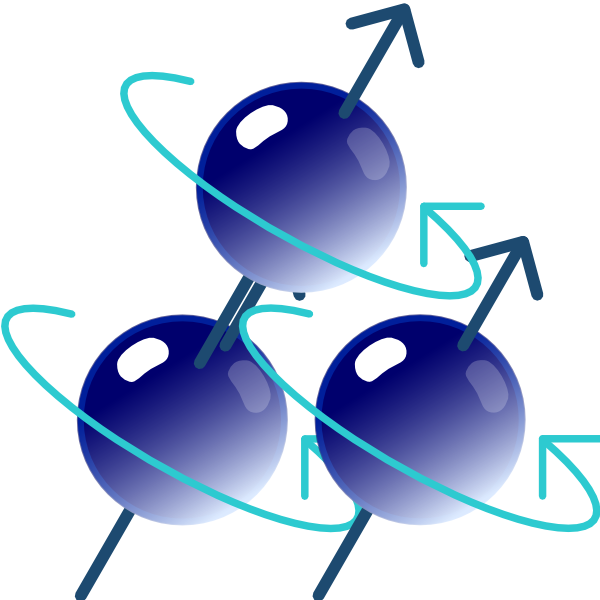
\includegraphics[width=3cm, bb=14 14 399 399]{graphics/misc/cluster_600x600}
\end{figure*}

Often in a relaxation dispersion analysis you will wish to fit a number of spin systems together using global parameters such as $\kex$, $\pA$, etc.
This can be achieved through the concept of clustering.
A cluster is defined by an ID string and can contain any number of spins.
Multiple clusters in one analysis can be defined.
Any spins not included in a cluster will be treated as a free spin whereby all parameters of the dispersion model are local to that spin.
Spin clusters can be defined using the \uf{relax\ufus{}disp\ufsep{}cluster} user function (see Section~\ref{uf: relax_disp.cluster} on page~\pageref{uf: relax_disp.cluster}) or via the spin cluster GUI element.

For the spin clustering, the special \uf{relax\ufus{}disp\ufsep{}parameter\ufus{}copy} user function has been designed to help avoid the impossibly large grid search.
This user function will copy the parameters from one non-clustered data pipe to another pipe, taking the median of the parameters from the first data pipe.
Rather than taking the median, the $\Rtwozero/\Ronerhoprime$ and $\dw$ related parameters which are independent of the clustering are simply copied.


% Grid search.
%~~~~~~~~~~~~~

\subsection{Dispersion parameter grid search}
\label{sect: Dispersion parameter grid search}

One of the most statistically unbiased methods for determining an initial parameter estimate prior to optimisation is to perform a grid search.
This is performed via the \uf{minimise.grid\ufus{}search} user function (see Section~\ref{uf: minimise.grid_search} on page~\pageref{uf: minimise.grid_search}).


For some dispersion models the grid search can be too computationally expensive.
In this case, some tricks can be used to bypass the parts of the grid search or the whole grid search:
\begin{description}
  \item[Model nesting:]  Using the optimised parameters of a simpler nested model as the starting point for optimisation.
  \item[Model equivalence:]  Using the optimised solution of an equivalent analytic model as the starting point for a numeric model.
\end{description}
These tricks are implemented in the relaxation dispersion auto-analysis protocol as described above.
If you do not use the auto-analysis or the GUI, then you are free to implement your own solutions.

The grid search lower and upper bounds default to:
\begin{subequations}
\begin{gather} 
    1 \leqslant \Rtwozero \leqslant 40, \\
    1 \leqslant \RtwozeroA \leqslant 40, \\
    1 \leqslant \RtwozeroB \leqslant 40, \\
    0 \leqslant \Phiex \leqslant 10, \\
    0 \leqslant \PhiexB \leqslant 10, \\
    0 \leqslant \PhiexC \leqslant 10, \\
    0 \leqslant \pA\dw^2 \leqslant 10, \\
    0 \leqslant \dw \leqslant 10, \\
    0 \leqslant \dwAB \leqslant 10, \\
    0 \leqslant \dwBC \leqslant 10, \\
    0 \leqslant \dwH \leqslant 3, \\
    0 \leqslant \dwHAB \leqslant 3, \\
    0 \leqslant \dwHBC \leqslant 3, \\
    0.5 \leqslant \pA \leqslant 1, \\
    0.0 \leqslant \pB \leqslant 0.5, \\
    0 \leqslant \kex \leqslant 1e^6, \\
    0 \leqslant \kexAB \leqslant 1e^6, \\
    0 \leqslant \kexBC \leqslant 1e^6, \\
    0 \leqslant \kA \leqslant 1e^6, \\
    0 \leqslant \kB \leqslant 1e^6, \\
    0 \leqslant \kAB \leqslant 1e^6, \\
    0 \leqslant \tex \leqslant 1e^{-6}.
\end{gather} 
\end{subequations}

For the MMQ models, the grid bounds are slightly different with
\begin{subequations}
\begin{gather} 
    -10 \leqslant \dw \leqslant 10, \\
    -10 \leqslant \dwAB \leqslant 10, \\
    -10 \leqslant \dwBC \leqslant 10, \\
    -3 \leqslant \dwH \leqslant 3, \\
    -3 \leqslant \dwHAB \leqslant 3, \\
    -3 \leqslant \dwHBC \leqslant 3.
\end{gather} 
\end{subequations}

These values can be changed when not using the auto-analysis.
Linear constraints can decrease the number of grid points searched through.



% Optimisation.
%~~~~~~~~~~~~~~

\subsection{Dispersion parameter optimisation}

For a description of gradients and Hessians, see Section~\ref{sect: gradient} on page~\pageref{sect: gradient} and Section~\ref{sect: Hessian} on page~\pageref{sect: Hessian} respectively.
The relaxation dispersion model gradients or Hessians have have either not been calculated for the analytic models or cannot be calculated as the solution is not analytic.
Numeric gradients and Hessians could be calculated but this is too computationally expensive, especially for the numeric models where this adds a second layer of numeric approximation.

Optimisation in relax is via the minfx package \url{https://gna.org/projects/minfx/}.
This allows the Nelder-Mead simplex optimisation technique (see Section~\ref{sect: Nelder-Mead simplex} on page~\pageref{sect: Nelder-Mead simplex}) and the log-barrier constraint algorithm (see Section~\ref{sect: Log-barrier constraint algorithm} on page~\pageref{sect: Log-barrier constraint algorithm}) to be used.
The advantage of these two techniques is that it enables extremely reliable and high precision optimisation without the use of gradients or Hessians, hence can significantly increase optimisation speeds.
They however do not avoid the multiple local minimum problem present in the MMQ models -- for that a highly accurate grid search is a reasonable solution.


% Constraints.
%~~~~~~~~~~~~~

\subsection{Relaxation dispersion parameter constraints}

To understand this section, please see Section~\ref{sect: constraint algorithms} on page~\pageref{sect: constraint algorithms}.
For a dispersion analysis, linear constraints are the most useful type of constraint.

For most models, the linear constraints in the notation of \eqref{eq: linear constraint} for the relaxation rates are
\begin{equation}
    \begin{pmatrix}
        1 & 0 & 0 \\
       -1 & 0 & 0 \\
        0 & 1 & 0 \\
        0 &-1 & 0 \\
        0 & 0 & 1 \\
        0 & 0 &-1 \\
    \end{pmatrix}
    \cdot
    \begin{pmatrix}
        \Rtwozero \\
        \RtwozeroA \\
        \RtwozeroB \\
    \end{pmatrix}
    \geqslant
    \begin{pmatrix}
        0 \\
        -200 \\
        0 \\
        -200 \\
        0 \\
        -200 \\
    \end{pmatrix},
\end{equation}

for the $\Phiex$ and $\dw$ parameters as
\begin{equation}
    \begin{pmatrix}
        1 & 0 & 0 & 0 & 0 & 0 & 0 & 0 & 0 & 0 \\
        0 & 1 & 0 & 0 & 0 & 0 & 0 & 0 & 0 & 0 \\
        0 & 0 & 1 & 0 & 0 & 0 & 0 & 0 & 0 & 0 \\
        0 & 0 & 0 & 1 & 0 & 0 & 0 & 0 & 0 & 0 \\
        0 & 0 & 0 & 0 & 1 & 0 & 0 & 0 & 0 & 0 \\
        0 & 0 & 0 & 0 & 0 & 1 & 0 & 0 & 0 & 0 \\
        0 & 0 & 0 & 0 & 0 & 0 & 1 & 0 & 0 & 0 \\
        0 & 0 & 0 & 0 & 0 & 0 & 0 & 1 & 0 & 0 \\
        0 & 0 & 0 & 0 & 0 & 0 & 0 & 0 & 1 & 0 \\
        0 & 0 & 0 & 0 & 0 & 0 & 0 & 0 & 0 & 1 \\
    \end{pmatrix}
    \cdot
    \begin{pmatrix}
        \Phiex \\
        \PhiexB \\
        \PhiexC \\
        \pA\dw^2 \\
        \dw \\
        \dwAB \\
        \dwBC \\
        \dwH \\
        \dwHAB \\
        \dwHBC \\
    \end{pmatrix}
    \geqslant
    \begin{pmatrix}
        0 \\
        0 \\
        0 \\
        0 \\
        0 \\
        0 \\
        0 \\
        0 \\
        0 \\
        0 \\
    \end{pmatrix},
\end{equation}

for the population parameters as
\begin{equation}
    \begin{pmatrix}
        -1 & 0 \\
         1 & 0 \\
         1 & 0 \\
        -1 &-1 \\
         1 & 2 \\
    \end{pmatrix}
    \cdot
    \begin{pmatrix}
        \pA \\
        \pB \\
    \end{pmatrix}
    \geqslant
    \begin{pmatrix}
        -1 \\
        0.5 \\
        0.85 \\
        -1 \\
        1 \\
    \end{pmatrix},
\end{equation}

and for the exchange rate and time parameters as
\begin{equation}
    \begin{pmatrix}
         1 & 0 & 0 & 0 & 0 & 0 & 0 \\
        -1 & 0 & 0 & 0 & 0 & 0 & 0 \\
         0 & 1 & 0 & 0 & 0 & 0 & 0 \\
         0 &-1 & 0 & 0 & 0 & 0 & 0 \\
         0 & 0 & 1 & 0 & 0 & 0 & 0 \\
         0 & 0 &-1 & 0 & 0 & 0 & 0 \\
         0 & 0 & 0 & 1 & 0 & 0 & 0 \\
         0 & 0 & 0 &-1 & 0 & 0 & 0 \\
         0 & 0 & 0 & 0 & 1 & 0 & 0 \\
         0 & 0 & 0 & 0 &-1 & 0 & 0 \\
         0 & 0 & 0 & 0 & 0 & 1 & 0 \\
         0 & 0 & 0 & 0 & 0 &-1 & 0 \\
         0 & 0 & 0 & 0 & 0 & 0 & 1 \\
    \end{pmatrix}
    \cdot
    \begin{pmatrix}
        \kex \\
        \kexAB \\
        \kexBC \\
        \kB \\
        \kC \\
        \kAB \\
        \tex \\
    \end{pmatrix}
    \geqslant
    \begin{pmatrix}
        0 \\
        -2e^6 \\
        0 \\
        -2e^6 \\
        0 \\
        -2e^6 \\
        0 \\
        -2e^6 \\
        0 \\
        -2e^6 \\
        0 \\
        -2e^6 \\
        0 \\
    \end{pmatrix}.
\end{equation}

\noindent  Through the isolation of each individual element, the constraints can be seen to be equivalent to
\begin{subequations}
\begin{gather} 
    0 \leqslant \Rtwozero \leqslant 200, \\
    0 \leqslant \RtwozeroA \leqslant 200, \\
    0 \leqslant \RtwozeroB \leqslant 200, \\
    \Phiex \geqslant 0, \\
    \PhiexB \geqslant 0, \\
    \PhiexC \geqslant 0, \\
    \dw \geqslant 0, \\
    \dwAB \geqslant 0, \\
    \dwBC \geqslant 0, \\
    \dwH \geqslant 0, \\
    \dwHAB \geqslant 0, \\
    \dwHBC \geqslant 0, \\
    \pA\dw^2 \geqslant 0, \\
    0 \leqslant \pA \leqslant 1, \\
    0 \leqslant \pB \leqslant \pA, \\
    0 \leqslant \pC \leqslant \pA, \\
    \pA \geqslant 0.85 \quad (\textrm{the skewed condition, } \pA \gg \pB), \\
    0 \leqslant \kex \leqslant 2e^6, \\
    0 \leqslant \kexAB \leqslant 2e^6, \\
    0 \leqslant \kexBC \leqslant 2e^6, \\
    0 \leqslant \kA \leqslant 2e^6, \\
    0 \leqslant \kB \leqslant 2e^6, \\
    0 \leqslant \kAB \leqslant 2e^6, \\
    \tex \geqslant 0.
\end{gather} 
\end{subequations}

Note that the $\dw$ and $\dwH$ constraints are not used for any of the MMQ-type models as sign differentiation is possible.
These constraints are also turned off for the `NS $\Ronerho$ 3-site linear' and `NS $\Ronerho$ 3-site' models.
And that the $\pA \geqslant 0.85$ constraint is used instead of the $\pA \geqslant 0.5$ constraint for all models which require $\pA \gg \pB$.
When not using the auto-analysis, constraints can be modified or turned off.


% Diagonal scaling.
%~~~~~~~~~~~~~~~~~~

\subsection{Relaxation dispersion diagonal scaling}

The concept of diagonal scaling is explained in Section~\ref{sect: diagonal scaling} on page~\pageref{sect: diagonal scaling}.

For the dispersion analysis the scaling factor of 10 is used for the relaxation rates, 1e$^5$ for the exchange rates, 1e$^{-4}$ for exchange times, and 1 for all other parameters.
The scaling matrix for the parameters \{$\Rtwozero$, $\RtwozeroA$, $\RtwozeroB$, $\Phiex$, $\PhiexB$, $\PhiexC$, $\pA\dw^2$, $\dw$, $\dwH$, $\pA$, $\pB$, $\kex$, $\kB$, $\kC$, $\kAB$, $\tex$\} is
\begin{equation}
    \begin{pmatrix}
        10 & 0  & 0  & 0 & 0 & 0 & 0 & 0 & 0 & 0 & 0 & 0    & 0    & 0    & 0    & 0       \\
        0  & 10 & 0  & 0 & 0 & 0 & 0 & 0 & 0 & 0 & 0 & 0    & 0    & 0    & 0    & 0       \\
        0  & 0  & 10 & 0 & 0 & 0 & 0 & 0 & 0 & 0 & 0 & 0    & 0    & 0    & 0    & 0       \\
        0  & 0  & 0  & 1 & 0 & 0 & 0 & 0 & 0 & 0 & 0 & 0    & 0    & 0    & 0    & 0       \\
        0  & 0  & 0  & 0 & 1 & 0 & 0 & 0 & 0 & 0 & 0 & 0    & 0    & 0    & 0    & 0       \\
        0  & 0  & 0  & 0 & 0 & 1 & 0 & 0 & 0 & 0 & 0 & 0    & 0    & 0    & 0    & 0       \\
        0  & 0  & 0  & 0 & 0 & 0 & 1 & 0 & 0 & 0 & 0 & 0    & 0    & 0    & 0    & 0       \\
        0  & 0  & 0  & 0 & 0 & 0 & 0 & 1 & 0 & 0 & 0 & 0    & 0    & 0    & 0    & 0       \\
        0  & 0  & 0  & 0 & 0 & 0 & 0 & 0 & 1 & 0 & 0 & 0    & 0    & 0    & 0    & 0       \\
        0  & 0  & 0  & 0 & 0 & 0 & 0 & 0 & 0 & 1 & 0 & 0    & 0    & 0    & 0    & 0       \\
        0  & 0  & 0  & 0 & 0 & 0 & 0 & 0 & 0 & 0 & 1 & 0    & 0    & 0    & 0    & 0       \\
        0  & 0  & 0  & 0 & 0 & 0 & 0 & 0 & 0 & 0 & 0 & 1e^5 & 0    & 0    & 0    & 0       \\
        0  & 0  & 0  & 0 & 0 & 0 & 0 & 0 & 0 & 0 & 0 & 0    & 1e^5 & 0    & 0    & 0       \\
        0  & 0  & 0  & 0 & 0 & 0 & 0 & 0 & 0 & 0 & 0 & 0    & 0    & 1e^5 & 0    & 0       \\
        0  & 0  & 0  & 0 & 0 & 0 & 0 & 0 & 0 & 0 & 0 & 0    & 0    & 0    & 1e^5 & 0       \\
        0  & 0  & 0  & 0 & 0 & 0 & 0 & 0 & 0 & 0 & 0 & 0    & 0    & 0    & 0    & 1e^{-4} \\
    \end{pmatrix}.
\end{equation}


% Model elimination.
%~~~~~~~~~~~~~~~~~~~

\subsection{Relaxation dispersion model elimination}
\label{sect: relaxation dispersion model elimination}

Relaxation dispersion models will often fail.
This may be due to data quality and quantity issues, inherent instability in certain models, or the use of analytic models outside of the range of their defined viability.
Model elimination is therefore required to remove these failed models prior to model selection, as failed models will often fit the experimental data statistically better than non-failed models.
The user function \uf{eliminate} (see Section~\ref{uf: eliminate} on page~\pageref{uf: eliminate}) is used to remove the failed models.
Model elimination was implement in relax as described in:

\begin{itemize}
  \item \bibentry{dAuvergneGooley06}
\end{itemize}

The following hard coded rules are used to eliminate models:
\begin{subequations}
\begin{gather} 
    \pA \leqslant 0.501, \\
    \pA \geqslant 0.999, \\
    \tex \geqslant 1.0.
\end{gather} 
\end{subequations}

If a parameter falls outside of these limits, the entire spin cluster will be deselected.
When not using the auto-analysis, custom model elimination rules can be defined and used with the \uf{eliminate} user function.


% MC elimination.
%~~~~~~~~~~~~~~~~

\subsection{Monte Carlo simulation elimination}

Just as models can fail, often Monte Carlo simulations will also experience optimisation failures (see Figure~4 of \citet{dAuvergneGooley06} for such a failure in the model-free optimisation space).
The minimum can be warped so much by the data randomisation that a new minimum appears at an unreasonable position in the optimisation space.
Even when the original model optimisation is successful, this can affect a small portion of the simulations.
These must be removed prior to calculating the parameter errors otherwise the errors will be significantly over estimated.
The simulation model failures are outliers which skew the error estimate, introducing a bias.
This can result in parameter error estimates which are too large.
The solution is the use of the \uf{eliminate} user function when Monte Carlo simulations are turned on -- this will automatically deselect simulations rather than spins using the rules from the previous section.
Note that relax is the only software which provides this feature.


% MPI.
%~~~~~

\subsection{Relaxation dispersion on a computer cluster using OpenMPI}
\label{sect: Relaxation dispersion using OpenMPI}

If the optimisation is too slow on a single computer, the dispersion analysis has been parallelised on the level of both the spin cluster and the Monte Carlo simulation.
The scaling efficiency is very close to perfect so if you have access to a computer cluster and the OpenMPI protocol, then the calculations can be run much faster.
The implementation uses Gary Thompson's multi-processor package.
See Section~\ref{sect: multi-processor} on page~\pageref{sect: multi-processor} for details on how to use this.



% TODO.
%%%%%%%

\section{To do -- dispersion features yet to be implemented}
\label{sect: dispersion: TODO}

The capabilities of the relaxation dispersion analysis in relax is expansive but it cannot be called complete.
There are a number of features and models yet to be implemented.
Missing features include:
\begin{itemize}
  \item The handling of off-resonance effects in the models of the numeric solution for CPMG-type data.
    This is specifically the `NS CPMG 2-site 3D' and `NS CPMG 2-site star' models and their `* full' equivalents.
    The necessary infrastructure is in place, but not activated yet (mainly due to a lack of synthetic data to test against).
    Currently only the software CATIA can handle this effect.
  \item Multi-state data -- the handling of data from two sets of peaks from the same spin system is not properly supported.
    It is currently handled by assuming each state is a separate spin system but this means that $\dw$, $\dwH$ and related parameters are not shared as they should be.
  \item The van't Hoff analysis of multi-temperature dispersion data (see \url{https://en.wikipedia.org/wiki/Van\_\%27t\_Hoff\_equation}).
  \item ZZ exchange.
  \item HD exchange.
  \item The \citet{Korzhnev05a} correction for constant-time $\Ronerho$ experiments for the analytic models ($\Ronerho$ = $-\lambda_1 -1/\Trelax\log{a_1}$, where $a_1$ = $1 - \pB\cos^2(\theta_A - \theta_B)$, and $\theta_A$ = $\arctan(\omegaone/\omegaA)$ and $\theta_B$ = $\arctan(\omegaone/\omegaB)$.
  \item Calculation of the dispersion $\alpha$ value from \cite{Millet00} (see \url{https://gna.org/task/?7800}).
  \item Support for CEST-type data.
  \item Offset support for the ground state chemical shift rather than the observed peak position.
    See \url{http://thread.gmane.org/gmane.science.nmr.relax.devel/5414/focus=5457}.
    This is really only needed for $\Ronerho$-type data.
\end{itemize}

If you would like one of these features, please contact the ``relax-devel at gna.org''\index{mailing list!relax-devel} mailing list.
The most useful would be if you have synthetic data whereby you know what the true solution should be.
This can then be incorporated into a relax system test and the feature implemented to allow the test to pass.
Note that such data should never be emailed to a public mailing list!
Synthetic data, or experimental data, can be obtained from the literature.

Some of the missing models include:
\begin{description}
  \item[`TP04':]\index{relaxation dispersion!TP04 model}  The $\Ronerho$-type data \citet{TrottPalmer04} N-site analytic equation for all time scales with parameters $\{\Ronerhoprime, \dots, \pone, \dots, \pN, \aveomega, \konetwo, \dots\, \koneN\}$.
  \item[`* $\Ronerho$':]  All of the 3-site and N-site models as summarised in Table~1 of \citet{PalmerMassi06}.
  \item[`BK13':]\index{relaxation dispersion!BK13 model}  The $\Ronerho$-type data \citet{Baldwin2013} off-resonance 2-site equation for all time scales with parameters $\{\Ronerhoprime, \dots, \pA, \dw, \kex\}$.  For details and code, see \url{https://gna.org/support/?3155}.
  \item[`BK13 full':]\index{relaxation dispersion!BK13 full model}  The $\Ronerho$-type data full \citet{Baldwin2013} off-resonance 2-site equation for all time scales with parameters $\{\RonerhoprimeA, \RonerhoprimeB, \dots, \pA, \dw, \kex\}$.  For details and code, see \url{https://gna.org/support/?3155}.
\end{description}

Information for how these can be added is given in the next section.


% Tutorial - adding models.
%%%%%%%%%%%%%%%%%%%%%%%%%%%

\section{Tutorial for adding relaxation dispersion models}
\label{sect: dispersion: model tutorial}

As the field of NMR relaxation dispersion has a very long history, it is not possible to include all analytic and numeric relaxation dispersion models for both CPMG-type\index{relaxation dispersion!CPMG-type experiment} or $\Ronerho$-type\index{relaxation dispersion!$\Ronerho$-type experiment} experiments in relax.
However it is not too difficult to add new models for your own needs if you have some Python, Matlab, Mathematica, or similar scripting skills.
The steps required are detailed on the \href{http://wiki.nmr-relax.com/}{relax wiki} page \url{http://wiki.nmr-relax.com/Tutorial\_for\_adding\_relaxation\_dispersion\_models\_to\_relax}.


% Software comparison.
%%%%%%%%%%%%%%%%%%%%%%

\section{Comparison of dispersion analysis software}
\label{sect: dispersion: software comparison}

Diverse software exists for analysing relaxation dispersion data.
The following is a list of the officially released software which you can use instead of relax:
\begin{description}
  \item[CPMGFit] Art Palmer's original dispersion analysis software at \url{http://www.palmer.hs.columbia.edu/software/cpmgfit.html}.
  \item[cpmg\_fit] Dmitry Korzhnev's dispersion software available upon request.
  \item[CATIA] Flemming Hansen's dispersion software at \url{http://www.biochem.ucl.ac.uk/hansen/catia/}.
    The reference is \citet{Hansen08}.
  \item[NESSY] Michael Bieri's dispersion software at \url{http://home.gna.org/nessy/}.
    The reference is \citet{BieriGooley11}.
  \item[GUARDD] Ian Kleckner's dispersion software at \url{http://code.google.com/p/guardd/}.
    The reference is \citet{KlecknerFoster12}.
  \item[ShereKhan] See the web server at \url{http://sherekhan.bionmr.org/}.
    The reference is \citet{Mazur13}.
  \item[GLOVE] Peter Wright's dispersion software at \url{http://www.scripps.edu/wright/}.
    The reference is \citet{Sugase13}.
  \item[chemex] Guillaume Bouvignies' dispersion software which can be found at \url{http://code.google.com/p/chemex/}.
\end{description}

There is currently support in relax for generating the input files for CPMGFit, CATIA, NESSY, and ShereKhan and for running CPMGFit and CATIA from within relax.

The features of the different software are compared in Table~\ref{table: dispersion software} on page~\pageref{table: dispersion software}.
Note that this table is likely to be incomplete so please see the websites of the respective software for an up to date list of features.
The aim of this table is to provide a fair comparison between all of the available dispersion software.
Therefore if you do find deficiencies or errors in this table please report these either to the relax users mailing list at ``relax-users at gna.org''\index{mailing list!relax-users}, submit a bug report\index{bug!report} (see section~\ref{reporting bugs} on page~\pageref{reporting bugs}), or send a private message to one of the relax developers (\url{http://gna.org/project/memberlist.php?group=relax}) so that the details can be corrected.

\clearpage
\begin{center}
\begin{small}

% The longtable environment.
\begin{latexonly}
\setlength\LTcapwidth{\textwidth}
\setlength\LTleft{0pt}
\setlength\LTright{0pt}
\end{latexonly}
\begin{longtable}{l@{\extracolsep{\fill}}ccccccccc}

% Caption.
\caption[Dispersion software comparison.]{Comparison of the features for the different dispersion software.}


% Header.
\\
\toprule
\vspace{25pt} \\
   & \begin{rotate}{45}CPMGFit\end{rotate} & \begin{rotate}{45}cpmg\_fit\end{rotate} & \begin{rotate}{45}CATIA\end{rotate} & \begin{rotate}{45}NESSY\end{rotate} & \begin{rotate}{45}GUARDD\end{rotate} & \begin{rotate}{45}ShereKhan\end{rotate} & \begin{rotate}{45}GLOVE\end{rotate} & \begin{rotate}{45}chemex\end{rotate} & \begin{rotate}{45}relax\end{rotate} \hspace{5pt} \\
%        & CPMGFit & CATIA & NESSY & GUARDD & ShereKhan & GLOVE & relax \\
\midrule
\endhead

% Footer.
\bottomrule
\endfoot

% Label.
\label{table: dispersion software}

%est row                    & \yes & \yes & \yes & \yes & \yes & \yes & \yes & \yes & \yes \\

% The models.
\vspace{-5pt} \\
\textbf{Dispersion models} \\
\cmidrule(lr){1-1}
\vspace{-5pt} \\
Base models \\
\cmidrule(lr){1-1}
$\Rtwoeff/\Ronerhoprime$    & \no  & \no  & \no  & \yes & \yes & \yes & \yes & \no  & \yes \\
No Rex                      & \no  & \yes & \no  & \yes & \yes & \no  & \yes & \no  & \yes \\

\vspace{-5pt} \\
Single quantum (SQ) CPMG-type \\
\cmidrule(lr){1-1}
LM63                        & \yes & \no  & \no  & \yes & \no  & \yes & \yes & \no  & \yes \\
LM63 3-site                 & \yes & \no  & \no  & \yes & \no  & \no  & \no  & \no  & \yes \\
CR72                        & \yes & \no  & \no  & \yes & \no  & \yes & \yes & \no  & \yes \\
IT99                        & \yes & \no  & \no  & \no  & \no  & \no  & \yes & \no  & \yes \\
TSMFK01                     & \no  & \no  & \no  & \no  & \no  & \no  & \no  & \no  & \yes \\
B14                         & \no  & \no  & \no  & \no  & \no  & \no  & \no  & \no  & \yes \\
NS 2-site                   & \no  & \yes & \yes & \no  & \no  & \yes & ?    & \no  & \yes \\

\vspace{-5pt} \\
MMQ (SQ, ZQ, DQ, \& MQ) CPMG-type \\
\cmidrule(lr){1-1}
MMQ CR72                    & \no  & \yes & \no  & \no  & \yes & \no  & ?    & \no  & \yes \\
NS MMQ 2-site               & \no  & \yes & \no  & \no  & \no  & \no  & ?    & \no  & \yes \\
NS MMQ 3-site linear        & \no  & \yes & \no  & \no  & \no  & \no  & ?    & \no  & \yes \\
NS MMQ 3-site               & \no  & \yes & \no  & \no  & \no  & \no  & ?    & \no  & \yes \\

\vspace{-5pt} \\
$\Ronerho$-type \\
\cmidrule(lr){1-1}
M61                         & \no  & \no  & \no  & \no  & \no  & \no  & \no  & \no  & \yes \\
DPL94                       & \no  & \no  & \no  & \no  & \no  & \no  & \no  & \no  & \yes \\
TP02                        & \no  & \yes & \no  & \no  & \no  & \no  & \no  & \no  & \yes \\
TAP03                       & \no  & \no  & \no  & \no  & \no  & \no  & \no  & \no  & \yes \\
TP04                        & \no  & \no  & \no  & \no  & \no  & \no  & \no  & \no  & \no  \\
MP05                        & \no  & \no  & \no  & \no  & \no  & \no  & \no  & \no  & \yes \\
B13                         & \no  & \no  & \no  & \no  & \no  & \no  & \no  & \no  & \no  \\
NS $\Ronerho$ 2-site        & \no  & \yes & \no  & \no  & \no  & \no  & ?    & \no  & \yes \\
NS $\Ronerho$ 3-site linear & \no  & \yes & \no  & \no  & \no  & \no  & \no  & \no  & \yes \\
NS $\Ronerho$ 3-site        & \no  & \yes & \no  & \no  & \no  & \no  & \no  & \no  & \yes \\

\midrule
\vspace{-5pt} \\
\textbf{General features} \\
\cmidrule(lr){1-1}
Parallelisation via MPI for running on clusters & \no  & \no  & \no  & \no  & \no  & \no  & \no  & \no  & \yes \\
Off-resonance effects (CPMG-type data)          & \no  & \no  & \yes & \no  & \no  & \no  & \no  & \no  & \no  \\
Off-resonance effects ($\Ronerho$-type data)    & \no  & \yes & \no  & \no  & \no  & \no  & \no  & \no  & \yes \\
Support for TROSY-type data                     & \no  & \no  & \yes & \no  & \no  & \no  & \no  & \no  & \no  \\
Support for CEST-type data                      & \no  & \no  & \no  & \no  & \no  & \no  & \no  & \yes & \no  \\
Support for scalar coupling effects             & \no  & \no  & \yes & \no  & \no  & \no  & \no  & \no  & \no  \\
Arrhenius / Van't Hoff analysis                 & \no  & \yes & \no  & \yes & \yes & \no  & \no  & \no  & \no  \\
ZZ exchange                                     & \no  & \no  & \no  & \no  & \no  & \no  & \no  & \no  & \no  \\
HD exchange                                     & \no  & \no  & \no  & \no  & \no  & \no  & \no  & \no  & \no  \\
Dispersion data back calculation (BC)           & \no  & \yes & \no  & \yes & \yes & \no  & \no  & \no  & \yes \\

\pagebreak

\vspace{-5pt} \\
\textbf{User interface} \\
\cmidrule(lr){1-1}
Graphical user interface (GUI)                  & \no  & \no  & \no  & \yes & \yes & \no  & \no  & \no  & \yes \\
Web user interface (Web UI)                     & \no  & \no  & \no  & \no  & \no  & \yes & \no  & \no  & \no  \\
Scripting user interface (Script UI)            & \no  & \yes & \yes & \no  & \no  & \yes & \yes & \no  & \yes \\
Shell interface                                 & \yes & \no  & \no  & \no  & \no  & \no  & \no  & \yes & \no  \\
Temperature and field-dependent simulator     \\
UI for experimental planning (data BC)          & \no  & \no  & \no  & \no  & \yes & \no  & \no  & \no  & \no  \\

\vspace{-5pt} \\
\textbf{Optimisation} \\
\cmidrule(lr){1-1}
Grid search algorithm                           & \yes & \no  & \no  & \yes & \yes & \yes & \yes & \no  & \yes \\
Grid search (via scripting)                     & \no  & \no  & \yes & \no  & \no  & \no  & \no  & \no  & \no  \\
Nelder-Mead simplex algorithm                   & \no  & \no  & \no  & \no  & \no  & \no  & \no  & \no  & \yes \\
Levenberg-Maquardt algorithm                    & \yes & \yes & \yes & \yes & \no  & \yes & \yes & \yes & \no  \\
Numeric gradient approximation                  & \yes & \yes & \yes & \yes & \no  & \yes & \yes & \yes & \no  \\
Logarithmic-barrier constraint algorithm        & \no  & \no  & \no  & \no  & \no  & \no  & \yes & \no  & \yes \\
MATLAB interior-point black magic               & \no  & \no  & \no  & \no  & \yes & \no  & \no  & \no  & \no  \\
Visualisation of the chi-squared space          & \no  & \no  & \no  & \no  & \yes & \no  & \no  & \no  & \yes \\

\vspace{-5pt} \\
\textbf{Error propagation} \\
\cmidrule(lr){1-1}
Covariance matrix (lowest quality)              & \yes & \yes & \yes & \no  & \yes & \yes & \yes & \no  & \no  \\
Jackknife simulations (for missing errors)      & \yes & \no  & \no  & \no  & \no  & \no  & \yes & \no  & \no  \\
Bootstrapping simulations (false errors)        & \no  & \no  & \no  & \no  & \no  & \no  & \no  & \no  & \no  \\
Monte Carlo simulations (gold standard)         & \yes & \no  & \no  & \yes & \yes & \no  & \yes & \yes & \yes \\

\vspace{-5pt} \\
\textbf{Inbuilt statistical comparisons} \\
\cmidrule(lr){1-1}
Akaike's Information Criterion (AIC)            & \no  & \no  & \no  & \yes & \no  & \no  & \no  & \no  & \yes \\
Small sample size AIC (AICc)                    & \no  & \no  & \no  & \yes & \no  & \no  & \no  & \no  & \yes \\
Bayesian Information Criterion (BIC)            & \no  & \no  & \no  & \no  & \no  & \no  & \no  & \no  & \yes \\
F-testing (ANOVA statistics)                    & \no  & \no  & \no  & \yes & \yes & \no  & \no  & \no  & \no  \\

\vspace{-5pt} \\
\textbf{Data and model testing} \\
\cmidrule(lr){1-1}
Insignificant dispersion curve tests            & \no  & \no  & \no  & \yes  & \no  & \no  & \no  & \no  & \yes \\
Model elimination tests                         & \no  & \no  & \no  & \no   & \no  & \no  & \no  & \no  & \yes \\

\vspace{-5pt} \\
\textbf{Programming languages} \\
\cmidrule(lr){1-1}
Python                      & \no  & \no  & \no  & \yes & \no  & \yes & \no  & \yes & \yes \\
C                           & \no  & \yes & \yes & \no  & \no  & \no  & \yes & \no  & \yes \\
Perl                        & \no  & \no  & \no  & \no  & \no  & \no  & \yes & \no  & \no  \\
MATLAB                      & \no  & \no  & \no  & \no  & \yes & \no  & \no  & \no  & \no  \\
FORTRAN                     & \yes & \no  & \no  & \no  & \no  & \no  & \no  & \no  & \no  \\
Ruby on Rails               & \no  & \no  & \no  & \no  & \no  & \yes & \no  & \no  & \no  \\

\vspace{-5pt} \\
\textbf{Open source licencing} \\
\cmidrule(lr){1-1}
GNU General Public Licence (version 2+)     & \yes & \no  & \no  & \no  & \no  & \no  & \no  & \no  & \no  \\
GNU General Public Licence (version 3+)     & \no  & \no  & \no  & \yes & \yes & \no  & \no  & \yes & \yes \\
Open source infrastructure                  & \no  & \no  & \no  & \yes & \yes & \no  & \no  & \yes & \yes \\
Proprietary                                 & \no  & \yes & \yes & \no  & \no  & \yes & \yes & \no  & \no  \\

\end{longtable}
\end{small}
\end{center}




% Script UI.
%%%%%%%%%%%%

\section{Analysing dispersion in the prompt/script UI mode}

Before reading this section, please read Chapter~\ref{ch: data model} covering the relax data model first.
It will explain many of the concepts used within the following example script.
For detailed information on how to run a relax script, please see section~\ref{sect: scripting} on page~\pageref{sect: scripting}.
The dispersion analysis is parallelised on the level of the spin cluster and Monte Carlo simulations so, if you have access to an MPI cluster or multi-core system with OpenMPI installed, please see section~\ref{sect: multi-processor} on page~\pageref{sect: multi-processor} for how to run the calculations much quicker.


% The sample script.
%~~~~~~~~~~~~~~~~~~~

\subsection{Dispersion script mode -- the sample script}

The following is a verbatim copy of the contents of the \file{sample\osus{}scripts\ossep{}relax\osus{}disp\ossep{}cpmg\osus{}analysis.py} file.
You will need to first copy this script to a dedicated analysis directory containing peak lists, a sequence or PDB file and a file listing unresolved spin systems, and then modify its contents to suit your specific analysis.
The script contents are:

\begin{lstlisting}
"""Script for performing a full relaxation dispersion analysis using CPMG-type data."""


# Python module imports.
from os import sep

# relax module imports.
from auto_analyses.relax_disp import Relax_disp


# Analysis variables.
#####################

# The dispersion models.
MODELS = ['R2eff', 'No Rex', 'CR72', 'N2 CPMG 2-site expanded']

# The grid search size (the number of increments per dimension).
GRID_INC = 11

# The number of Monte Carlo simulations to be used for error analysis at the end of the analysis.
MC_NUM = 500

# The results directory.
RESULTS_DIR = '.'

# The model selection technique to use.
MODSEL = 'AIC'

# The flag for only using numeric models in the final model selection.
NUMERIC_ONLY = False

# The R2eff value in rad/s by which to judge insignificance.  If the maximum difference between two points on all dispersion curves for a spin is less than this value, that spin will be deselected.
INSIGNIFICANCE = 1.0



# Set up the data pipe.
#######################

# Create the data pipe.
pipe_name = 'base pipe'
pipe_bundle = 'relax_disp'
pipe.create(pipe_name=pipe_name, bundle=pipe_bundle, pipe_type='relax_disp')

# Load the sequence.
sequence.read('fake_sequence.in', res_num_col=1, res_name_col=2)

# Name the spins so they can be matched to the assignments, and the isotope for field strength scaling.
spin.name(name='N')
spin.isotope(isotope='15N')

# The spectral data - spectrum ID, peak list file name, CPMG frequency (Hz), spectrometer frequency in Hertz.
data = [
    ['500_reference.in',    '500_MHz'+sep+'reference.in_sparky',           None,  500e6],
    ['500_66.667.in',       '500_MHz'+sep+'66.667.in_sparky',           66.6666,  500e6],
    ['500_133.33.in',       '500_MHz'+sep+'133.33.in_sparky',          133.3333,  500e6],
    ['500_133.33.in.bis',   '500_MHz'+sep+'133.33.in.bis_sparky',      133.3333,  500e6],
    ['500_200.in',          '500_MHz'+sep+'200.in_sparky',             200.0000,  500e6],
    ['500_266.67.in',       '500_MHz'+sep+'266.67.in_sparky',          266.6666,  500e6],
    ['500_333.33.in',       '500_MHz'+sep+'333.33.in_sparky',          333.3333,  500e6],
    ['500_400.in',          '500_MHz'+sep+'400.in_sparky',             400.0000,  500e6],
    ['500_466.67.in',       '500_MHz'+sep+'466.67.in_sparky',          466.6666,  500e6],
    ['500_533.33.in',       '500_MHz'+sep+'533.33.in_sparky',          533.3333,  500e6],
    ['500_533.33.in.bis',   '500_MHz'+sep+'533.33.in.bis_sparky',      533.3333,  500e6],
    ['500_600.in',          '500_MHz'+sep+'600.in_sparky',             600.0000,  500e6],
    ['500_666.67.in',       '500_MHz'+sep+'666.67.in_sparky',          666.6666,  500e6],
    ['500_733.33.in',       '500_MHz'+sep+'733.33.in_sparky',          733.3333,  500e6],
    ['500_800.in',          '500_MHz'+sep+'800.in_sparky',             800.0000,  500e6],
    ['500_866.67.in',       '500_MHz'+sep+'866.67.in_sparky',          866.6666,  500e6],
    ['500_933.33.in',       '500_MHz'+sep+'933.33.in_sparky',          933.3333,  500e6],
    ['500_933.33.in.bis',   '500_MHz'+sep+'933.33.in.bis_sparky',      933.3333,  500e6],
    ['500_1000.in',         '500_MHz'+sep+'1000.in_sparky',           1000.0000,  500e6],
    ['800_reference.in',    '800_MHz'+sep+'reference.in_sparky',           None,  800e6],
    ['800_66.667.in',       '800_MHz'+sep+'66.667.in_sparky',           66.6666,  800e6],
    ['800_133.33.in',       '800_MHz'+sep+'133.33.in_sparky',          133.3333,  800e6],
    ['800_133.33.in.bis',   '800_MHz'+sep+'133.33.in.bis_sparky',      133.3333,  800e6],
    ['800_200.in',          '800_MHz'+sep+'200.in_sparky',             200.0000,  800e6],
    ['800_266.67.in',       '800_MHz'+sep+'266.67.in_sparky',          266.6666,  800e6],
    ['800_333.33.in',       '800_MHz'+sep+'333.33.in_sparky',          333.3333,  800e6],
    ['800_400.in',          '800_MHz'+sep+'400.in_sparky',             400.0000,  800e6],
    ['800_466.67.in',       '800_MHz'+sep+'466.67.in_sparky',          466.6666,  800e6],
    ['800_533.33.in',       '800_MHz'+sep+'533.33.in_sparky',          533.3333,  800e6],
    ['800_533.33.in.bis',   '800_MHz'+sep+'533.33.in.bis_sparky',      533.3333,  800e6],
    ['800_600.in',          '800_MHz'+sep+'600.in_sparky',             600.0000,  800e6],
    ['800_666.67.in',       '800_MHz'+sep+'666.67.in_sparky',          666.6666,  800e6],
    ['800_733.33.in',       '800_MHz'+sep+'733.33.in_sparky',          733.3333,  800e6],
    ['800_800.in',          '800_MHz'+sep+'800.in_sparky',             800.0000,  800e6],
    ['800_866.67.in',       '800_MHz'+sep+'866.67.in_sparky',          866.6666,  800e6],
    ['800_933.33.in',       '800_MHz'+sep+'933.33.in_sparky',          933.3333,  800e6],
    ['800_933.33.in.bis',   '800_MHz'+sep+'933.33.in.bis_sparky',      933.3333,  800e6],
    ['800_1000.in',         '800_MHz'+sep+'1000.in_sparky',           1000.0000,  800e6]
]

# Loop over the spectra.
for id, file, cpmg_frq, H_frq in data:
    # Load the peak intensities.
    spectrum.read_intensities(file=file, spectrum_id=id, int_method='height')

    # Set the relaxation dispersion experiment type.
    relax_disp.exp_type(spectrum_id=id, exp_type='SQ CPMG')

    # Set the relaxation dispersion CPMG frequencies.
    relax_disp.cpmg_setup(spectrum_id=id, cpmg_frq=cpmg_frq)

    # Set the NMR field strength of the spectrum.
    spectrometer.frequency(id=id, frq=H_frq)

    # Relaxation dispersion CPMG constant time delay T (in s).
    relax_disp.relax_time(spectrum_id=id, time=0.030)

# Specify the duplicated spectra.
spectrum.replicated(spectrum_ids=['500_133.33.in', '500_133.33.in.bis'])
spectrum.replicated(spectrum_ids=['500_533.33.in', '500_533.33.in.bis'])
spectrum.replicated(spectrum_ids=['500_933.33.in', '500_933.33.in.bis'])
spectrum.replicated(spectrum_ids=['800_133.33.in', '800_133.33.in.bis'])
spectrum.replicated(spectrum_ids=['800_533.33.in', '800_533.33.in.bis'])
spectrum.replicated(spectrum_ids=['800_933.33.in', '800_933.33.in.bis'])

# Peak intensity error analysis.
spectrum.error_analysis(subset=['500_reference.in', '500_66.667.in', '500_133.33.in', '500_133.33.in.bis', '500_200.in', '500_266.67.in', '500_333.33.in', '500_400.in', '500_466.67.in', '500_533.33.in', '500_533.33.in.bis', '500_600.in', '500_666.67.in', '500_733.33.in', '500_800.in', '500_866.67.in', '500_933.33.in', '500_933.33.in.bis', '500_1000.in'])
spectrum.error_analysis(subset=['800_reference.in', '800_66.667.in', '800_133.33.in', '800_133.33.in.bis', '800_200.in', '800_266.67.in', '800_333.33.in', '800_400.in', '800_466.67.in', '800_533.33.in', '800_533.33.in.bis', '800_600.in', '800_666.67.in', '800_733.33.in', '800_800.in', '800_866.67.in', '800_933.33.in', '800_933.33.in.bis', '800_1000.in'])

# Deselect unresolved spins.
deselect.read(file='unresolved', dir='500_MHz', res_num_col=1)
deselect.read(file='unresolved', dir='800_MHz', res_num_col=1)



# Auto-analysis execution.
##########################

# Do not change!
Relax_disp(pipe_name=pipe_name, pipe_bundle=pipe_bundle, results_dir=RESULTS_DIR, models=MODELS, grid_inc=GRID_INC, mc_sim_num=MC_NUM, modsel=MODSEL, insignificance=INSIGNIFICANCE, numeric_only=NUMERIC_ONLY)
\end{lstlisting}


% The imports.
%~~~~~~~~~~~~~

\subsection{Dispersion script mode -- imports} \label{sect: dispersion script imports}

At the very start of the script are two import statements.
This is simply the standard Python import system for modules.
The first will import the \pycode{sep} variable which is the operating system independent directory separator:

\begin{lstlisting}[firstnumber=4]
# Python module imports.
from os import sep
\end{lstlisting}

This \pycode{sep} variable will be used later on in the script.
The second import is that of the automated relaxation dispersion class \pycode{Relax\_disp} which will be used at the very end of the script to perform the full analysis:

\begin{lstlisting}[firstnumber=7]
# relax module imports.
from auto_analyses.relax_disp import Relax_disp
\end{lstlisting}


% The analysis variables.
%~~~~~~~~~~~~~~~~~~~~~~~~

\subsection{Dispersion script mode -- analysis variables} \label{sect: dispersion script variables}

The next part of the script is the definition of a number of analysis variables.
As the example in this section is for CPMG-type experiments, the relaxation dispersion models which will be used in the auto-analysis are:

\begin{lstlisting}[firstnumber=14]
# The dispersion models.
MODELS = ['R2eff', 'No Rex', 'CR72', 'N2 CPMG 2-site expanded']
\end{lstlisting}

This list can be expanded to most of the 2-site exchange models, for example as:

\begin{lstlisting}[numbers=none]
MODELS = ['R2eff', 'No Rex', 'LM63', 'CR72', 'IT99', 'TSMFK01', 'NS CPMG 2-site expanded']
\end{lstlisting}

But note that the selection of which models to use is incredibly important.
Do not use models which are not suitable for the data as that will cause the final results to contain rubbish.
If you have $\Ronerho$-type off-resonance data, the models could be changed to:

\begin{lstlisting}[numbers=none]
MODELS = ['R2eff', 'No Rex', 'DPL94', 'NS R1rho 2-site']
\end{lstlisting}

The next variable affects the optimisation precision:

\begin{lstlisting}[firstnumber=17]
# The grid search size (the number of increments per dimension).
GRID_INC = 21
\end{lstlisting}

The number of grid search increments may be decreased, but only after careful checking with a higher number of increments.
Setting this value too low may place the initial optimisation too far away from the minimum.
Although as-of-yet undetected and unpublished, if multiple local minima do exist then optimisation may not reach the global minimum.
Too little grid search increments can also cause the total optimisation time to increase as the Nelder-Mead simplex\index{optimisation!simplex algorithm}\index{optimisation!Nelder-Mead algorithm} optimisation together with the Logarithmic-barrier penalty function\index{optimisation!logarithmic-barrier penalty function} as used in the auto-analysis may require more time to reach the minimum.

The Monte Carlo simulation\index{Monte Carlo simulation} number \pycode{MC\_NUM} variable affects the error estimate precision:

\begin{lstlisting}[firstnumber=20]
# The number of Monte Carlo simulations to be used for error analysis at the end of the analysis.
MC_NUM = 500
\end{lstlisting}

For accurate parameter errors this number should not be decreased.
Ideally it should be increased however this will significantly increase the total analysis time.
The next variable allows you to change the directory in which all results files from the auto-analysis will be saved.

\begin{lstlisting}[firstnumber=23]
# The results directory.
RESULTS_DIR = '.'
\end{lstlisting}

The \pycode{MODSEL} variable defines how the best dispersion model for the measured data is chosen:

\begin{lstlisting}[firstnumber=26]
# The model selection technique to use.
MODSEL = 'AIC'
\end{lstlisting}

For the automated analysis, currently only AIC\index{model selection!AIC}, AICc\index{model selection!AICc}, and BIC\index{model selection!BIC} are supported.
For details about these frequentist\index{model selection!frequentist} model selection techniques and their application to NMR data, see \citet{dAuvergneGooley03}.
Post-analysis comparisons can also be preformed if desired.
The \pycode{NUMERIC\_ONLY} variable can be used to choose if only numeric or all models will be used in the model selection for the final results:

\begin{lstlisting}[firstnumber=29]
# The flag for only using numeric models in the final model selection.
NUMERIC_ONLY = False
\end{lstlisting}

To only use numeric models in the model selection while allowing models such as 'CR72' to be optimised and used as the starting point for the numeric models, change this variable to:

\begin{lstlisting}[numbers=none]
NUMERIC_ONLY = True
\end{lstlisting}

The last variable allows spins with insignificant dispersion profiles to be deselected:

\begin{lstlisting}[firstnumber=32]
# The R2eff value in rad/s by which to judge insignificance.  If the maximum difference between two points on all dispersion curves for a spin is less than this value, that spin will be deselected.
INSIGNIFICANCE = 1.0
\end{lstlisting}

This is often needed due to the errors in the dispersion curves being underestimated, hence the 'No Rex' model is not selected when clearly it should be.
To use all data in the analysis, this variable should be set to 0.0.


% Initialisation of the data pipe.
%~~~~~~~~~~~~~~~~~~~~~~~~~~~~~~~~~

\subsection{Dispersion script mode -- initialisation of the data pipe} \label{sect: dispersion initialisation}

The data pipe is created using the lines:

\begin{lstlisting}[firstnumber=40]
# Create the data pipe.
pipe_name = 'base pipe'
pipe_bundle = 'relax_disp'
pipe.create(pipe_name=pipe_name, bundle=pipe_bundle, pipe_type='relax_disp')
\end{lstlisting}

The first two lines define variables for the data pipe name and the pipe bundle name.
The pipe bundle is used to group together all of the data pipes created by the automated protocol.
See section~\ref{sect: data pipe bundles} on page~\pageref{sect: data pipe bundles} for more details.

The \uf{pipe\ufsep{}create} user function will then create a relaxation dispersion specific data pipe labelled with the pipe and bundle names.
The third argument sets the pipe type to that of relaxation dispersion.
The rest of the script is used to fill this base data pipe with all of the data required for a dispersion analysis.
The auto-analysis will then copy the data from this pipe as it sees fit.


% Spin systems.
%~~~~~~~~~~~~~~

\subsection{Dispersion script mode -- setting up the spin systems}

The first thing which needs to be completed prior to any spin specific command is to generate the molecule, residue and spin data structures for storing the spin specific data.
In the sample script above, this is generated from a plain text file with the sequence information, however a PDB file can be used instead (see the \uf{structure\ufsep{}read\ufus{}pdb} user function on page~\pageref{uf: structure.read_pdb} for more details).
In the case of the sample script, the command:

\begin{lstlisting}[firstnumber=45]
# Load the sequence.
sequence.read('fake_sequence.in', res_num_col=1, res_name_col=2)
\end{lstlisting}

will load residue names and numbers from the \file{fake\osus{}sequence.in} file into relax, creating one spin per residue.
Then:

\begin{lstlisting}[firstnumber=48]
# Name the spins so they can be matched to the assignments, and the isotope for field strength scaling.
spin.name(name='N')
spin.isotope(isotope='15N')
\end{lstlisting}

will set up the spin information required for loading the peak intensity data from Sparky peak lists and for the analysis of the dispersion data.


% Loading the data.
%~~~~~~~~~~~~~~~~~~

\subsection{Dispersion script mode -- loading the data}

To load the peak intensities\index{peak!intensity} into relax, a large data structure is first defined:

\begin{lstlisting}[firstnumber=52]
# The spectral data - spectrum ID, peak list file name, CPMG frequency (Hz), spectrometer frequency in Hertz.
data = [
    ['500_reference.in',    '500_MHz'+sep+'reference.in_sparky',           None,  500e6],
    ['500_66.667.in',       '500_MHz'+sep+'66.667.in_sparky',           66.6666,  500e6],
    ['500_133.33.in',       '500_MHz'+sep+'133.33.in_sparky',          133.3333,  500e6],
    ['500_133.33.in.bis',   '500_MHz'+sep+'133.33.in.bis_sparky',      133.3333,  500e6],
    ['500_200.in',          '500_MHz'+sep+'200.in_sparky',             200.0000,  500e6],
    ['500_266.67.in',       '500_MHz'+sep+'266.67.in_sparky',          266.6666,  500e6],
    ['500_333.33.in',       '500_MHz'+sep+'333.33.in_sparky',          333.3333,  500e6],
    ['500_400.in',          '500_MHz'+sep+'400.in_sparky',             400.0000,  500e6],
    ['500_466.67.in',       '500_MHz'+sep+'466.67.in_sparky',          466.6666,  500e6],
    ['500_533.33.in',       '500_MHz'+sep+'533.33.in_sparky',          533.3333,  500e6],
    ['500_533.33.in.bis',   '500_MHz'+sep+'533.33.in.bis_sparky',      533.3333,  500e6],
    ['500_600.in',          '500_MHz'+sep+'600.in_sparky',             600.0000,  500e6],
    ['500_666.67.in',       '500_MHz'+sep+'666.67.in_sparky',          666.6666,  500e6],
    ['500_733.33.in',       '500_MHz'+sep+'733.33.in_sparky',          733.3333,  500e6],
    ['500_800.in',          '500_MHz'+sep+'800.in_sparky',             800.0000,  500e6],
    ['500_866.67.in',       '500_MHz'+sep+'866.67.in_sparky',          866.6666,  500e6],
    ['500_933.33.in',       '500_MHz'+sep+'933.33.in_sparky',          933.3333,  500e6],
    ['500_933.33.in.bis',   '500_MHz'+sep+'933.33.in.bis_sparky',      933.3333,  500e6],
    ['500_1000.in',         '500_MHz'+sep+'1000.in_sparky',           1000.0000,  500e6],
    ['800_reference.in',    '800_MHz'+sep+'reference.in_sparky',           None,  800e6],
    ['800_66.667.in',       '800_MHz'+sep+'66.667.in_sparky',           66.6666,  800e6],
    ['800_133.33.in',       '800_MHz'+sep+'133.33.in_sparky',          133.3333,  800e6],
    ['800_133.33.in.bis',   '800_MHz'+sep+'133.33.in.bis_sparky',      133.3333,  800e6],
    ['800_200.in',          '800_MHz'+sep+'200.in_sparky',             200.0000,  800e6],
    ['800_266.67.in',       '800_MHz'+sep+'266.67.in_sparky',          266.6666,  800e6],
    ['800_333.33.in',       '800_MHz'+sep+'333.33.in_sparky',          333.3333,  800e6],
    ['800_400.in',          '800_MHz'+sep+'400.in_sparky',             400.0000,  800e6],
    ['800_466.67.in',       '800_MHz'+sep+'466.67.in_sparky',          466.6666,  800e6],
    ['800_533.33.in',       '800_MHz'+sep+'533.33.in_sparky',          533.3333,  800e6],
    ['800_533.33.in.bis',   '800_MHz'+sep+'533.33.in.bis_sparky',      533.3333,  800e6],
    ['800_600.in',          '800_MHz'+sep+'600.in_sparky',             600.0000,  800e6],
    ['800_666.67.in',       '800_MHz'+sep+'666.67.in_sparky',          666.6666,  800e6],
    ['800_733.33.in',       '800_MHz'+sep+'733.33.in_sparky',          733.3333,  800e6],
    ['800_800.in',          '800_MHz'+sep+'800.in_sparky',             800.0000,  800e6],
    ['800_866.67.in',       '800_MHz'+sep+'866.67.in_sparky',          866.6666,  800e6],
    ['800_933.33.in',       '800_MHz'+sep+'933.33.in_sparky',          933.3333,  800e6],
    ['800_933.33.in.bis',   '800_MHz'+sep+'933.33.in.bis_sparky',      933.3333,  800e6],
    ['800_1000.in',         '800_MHz'+sep+'1000.in_sparky',           1000.0000,  800e6]
]
\end{lstlisting}

In Python terminology, this is a list of lists data structure.
It is essentially a matrix of information which is used in the subsequent \pycode{for} loop.
The comment explains what each element is.
For $\Ronerho$-type experiments, the CPMG frequency column can be replaced with the spin-lock field strength.
This data structure will need to be tailored to your data.
It can be seen that the \pycode{sep} variable is now being used to specify that the Sparky files are either located in the \directory{500\osus{}MHz} or \directory{800\osus{}MHz} directories.
It is used here to make this script independent of the operating system.

The Python \pycode{for} loop starts with the lines:

\begin{lstlisting}[firstnumber=94]
# Loop over the spectra.
for id, file, cpmg_frq, H_frq in data:
\end{lstlisting}

and includes all subsequently indented lines.
This line of code takes the elements of the \pycode{data} data structure and splits it into 4 variables.
Therefore for the first line, \pycode{id} will be set to \pycode{`500\_reference.in'}, \pycode{file} will be set to \pycode{`500\_MHz/reference.in\_sparky'} on a Linux machine, \pycode{cpmg\_frq} will be \pycode{None}, and \pycode{H\_frq} will be 500~MHz.
For $\Ronerho$-type data, you could change the \pycode{cpmg\_frq} variable to \pycode{field} for example.

The first user function in the block loads the peak intensity data from the peak lists:

\begin{lstlisting}[firstnumber=96]
    # Load the peak intensities.
    spectrum.read_intensities(file=file, spectrum_id=id, int_method='height')
\end{lstlisting}

This assumes that peak heights were measured.
All data will be tagged with the given ID string.
For examples of peak list formats supported by relax, see Section~\ref{sect: Rx data loading} on page~\pageref{sect: Rx data loading}.
The next step is to specify the dispersion experiment type for each spectrum:

\begin{lstlisting}[firstnumber=99]
    # Set the relaxation dispersion experiment type.
    relax_disp.exp_type(spectrum_id=id, exp_type='SQ CPMG')
\end{lstlisting}

This can be \pycode{`SQ CPMG'}, \pycode{`DQ CPMG'},  \pycode{`ZQ CPMG'},  \pycode{`MQ CPMG'},  \pycode{`1H SQ CPMG'}, \pycode{`1H MQ CPMG'} or \pycode{`R1rho'}.
The next user function sets the CPMG frequencies for each spectrum:

\begin{lstlisting}[firstnumber=102]
    # Set the relaxation dispersion CPMG frequencies.
    relax_disp.cpmg_setup(spectrum_id=id, cpmg_frq=cpmg_frq)
\end{lstlisting}

For an $\Ronerho$-type experiment, these lines could be changed to:

\begin{lstlisting}[numbers=none]
    # Set the relaxation dispersion R1rho spin lock field strength.
    relax_disp.spin_lock_field(spectrum_id=id, field=field)
\end{lstlisting}

Then the NMR spectrometer field strength is set:

\begin{lstlisting}[firstnumber=105]
    # Set the NMR field strength of the spectrum.
    spectrometer.frequency(id=id, frq=H_frq)
\end{lstlisting}

And finally the relaxation time period is set with:

\begin{lstlisting}[firstnumber=108]
    # Relaxation dispersion CPMG constant time delay T (in s).
    relax_disp.relax_time(spectrum_id=id, time=0.030)
\end{lstlisting}

If exponential data has been collected rather than fixed time period data, then the \pycode{data} data structure can have an additional column added for the relaxation times, and then this same user function can be used.
The \pycode{for} loop will need one extra variable for the times, and this should be passed into this \uf{relax\ufus{}disp\ufsep{}relax\ufus{}time} user function for the time argument.

Finally, once the \pycode{for} loop has completed, replicated spectra are defined with the commands:

\begin{lstlisting}[firstnumber=111]
# Specify the duplicated spectra.
spectrum.replicated(spectrum_ids=['500_133.33.in', '500_133.33.in.bis'])
spectrum.replicated(spectrum_ids=['500_533.33.in', '500_533.33.in.bis'])
spectrum.replicated(spectrum_ids=['500_933.33.in', '500_933.33.in.bis'])
spectrum.replicated(spectrum_ids=['800_133.33.in', '800_133.33.in.bis'])
spectrum.replicated(spectrum_ids=['800_533.33.in', '800_533.33.in.bis'])
spectrum.replicated(spectrum_ids=['800_933.33.in', '800_933.33.in.bis'])
\end{lstlisting}


% The rest of the setup.
%~~~~~~~~~~~~~~~~~~~~~~~

\subsection{Dispersion script mode -- the rest of the setup} \label{sect: dispersion setup fin}

Once all the peak intensity data has been loaded a few calculations are required prior to optimisation.
Firstly the peak intensities for individual spins needs to be averaged across replicated spectra.
The peak intensity errors also have to be calculated using the standard deviation formula.
These two operations are executed by the user functions:

\begin{lstlisting}[firstnumber=119]
# Peak intensity error analysis.
spectrum.error_analysis(subset=['500_reference.in', '500_66.667.in', '500_133.33.in', '500_133.33.in.bis', '500_200.in', '500_266.67.in', '500_333.33.in', '500_400.in', '500_466.67.in', '500_533.33.in', '500_533.33.in.bis', '500_600.in', '500_666.67.in', '500_733.33.in', '500_800.in', '500_866.67.in', '500_933.33.in', '500_933.33.in.bis', '500_1000.in'])
spectrum.error_analysis(subset=['800_reference.in', '800_66.667.in', '800_133.33.in', '800_133.33.in.bis', '800_200.in', '800_266.67.in', '800_333.33.in', '800_400.in', '800_466.67.in', '800_533.33.in', '800_533.33.in.bis', '800_600.in', '800_666.67.in', '800_733.33.in', '800_800.in', '800_866.67.in', '800_933.33.in', '800_933.33.in.bis', '800_1000.in'])
\end{lstlisting}

Here the 500~MHz and 800~MHz peak intensity errors have been calculated separately as they should not be the same.

Any spins which cannot be resolved due to peak overlap were included in a file called \file{unresolved}.
This file can consist of optional columns of the molecule name, the residue name and number, and the spin name and number.
The matching spins are excluded from the analysis by the user functions:

\begin{lstlisting}[firstnumber=123]
# Deselect unresolved spins.
deselect.read(file='unresolved', dir='500_MHz', res_num_col=1)
deselect.read(file='unresolved', dir='800_MHz', res_num_col=1)
\end{lstlisting}


% Execution.
%~~~~~~~~~~~
\subsection{Dispersion script mode -- execution}

Once the data has set up and you have modified your script to match your analysis needs, then the data pipe, pipe bundle and analysis variables are passed into the \module{Relax\pyus{}disp} class.
This is the final lines of the script:

\begin{lstlisting}[firstnumber=129]
# Auto-analysis execution.
##########################

# Do not change!
Relax_disp(pipe_name=pipe_name, pipe_bundle=pipe_bundle, results_dir=RESULTS_DIR, models=MODELS, grid_inc=GRID_INC, mc_sim_num=MC_NUM, modsel=MODSEL, insignificance=INSIGNIFICANCE, numeric_only=NUMERIC_ONLY)
\end{lstlisting}

This will start the auto-analysis.
If you are adventurous, you can replace this line with your own \uf{minimise.grid\ufus{}search}, \uf{minimise.execute}, and \uf{monte\ufus{}carlo\ufsep{}*} user function calls and design your own protocol.
For ideas in designing your own advanced analysis, see the \file{auto\osus{}analysis\ossep{}relax\osus{}disp.py} file.



% GUI.
%%%%%%

\newpage
\section{The relaxation dispersion auto-analysis in the GUI}

The following demonstration of the relaxation dispersion analysis in the graphical user interface (GUI) uses the experimental single quantum (SQ) CPMG-type data from Flemming Hansen located in the relax directory \directory{test\osus{}suite\ossep{}shared\osus{}data\ossep{}dispersion\ossep{}Hansen}.
This is the data from the paper:
\begin{itemize}
  \item \bibentry{Hansen08}
\end{itemize}

More details can be seen in the \file{README} file in that directory.
By using the data in this directory and following the instructions below, a complete dispersion analysis can be performed.

Note that the dispersion analysis in the GUI uses the automated protocol as implemented in the \file{auto\osus{}analyses\ossep{}relax\osus{}disp.py} relax script.
If you wish to perform a custom analysis or implement your own protocol, please use the prompt/scripting user interface instead to have access to the full flexibility and power of relax.

When running the analysis, it is best to keep a permanent log of all of the printouts, warnings, errors and messages produced by relax.
Such information will be an invaluable reference when comparing the non-clustered and clustered results, as well as understanding what happened to each spin system under study.
This can be achieved by running relax with the command line options:

\example{\$ relax --log log --gui}

All output from relax will then be visible both in the relax controller window (see Figure~\ref{fig: screenshot: relax controller} on page~\pageref{fig: screenshot: relax controller}) and in the \file{log} file.
Other relax options can be seen by running:

\example{\$ relax --help}


% Two analyses.
%~~~~~~~~~~~~~~

\subsection{Dispersion GUI mode -- two analyses}

To process this test data, two separate analyses will be performed:
\begin{itemize}
  \item The first analysis will consists of treating all spins independently from each other.
    This will use model selection to determine if any statistically significant relaxation dispersion is present by comparing to the `No Rex' dispersion model.
  \item The second analysis will consists of clustering spins with similar kinetics and thermodynamics parameters (exchange rates and populations respectively) and optimising these clusters using a common set of exchange parameters.
\end{itemize}

In this example, Gary Thompson's multiprocessor framework (see section~\ref{sect: Relaxation dispersion using OpenMPI} on page~\pageref{sect: Relaxation dispersion using OpenMPI}) will be used with OpenMPI\index{MPI!OpenMPI} on a single four-core, hyper-threaded computer with the command:

\example{\$ mpirun -np 8 /data/relax/relax-trunk/relax --multi='mpi4py' --log $\sim$/tmp/dispersion/log\_non\_clustered --gui}

Note that the \directory{$\sim$\ossep{}tmp\ossep{}dispersion} directory should be created before starting relax.
If running on a system where your home directory is not defined as \directory{$\sim$\ossep{}}, MS Windows for example, the \directory{$\sim$} part will need to be replaced with some other directory.
A different command will be used for the clustered analysis to store the log messages in a separate file.
The two logs will be used to compare the two analysis types at the end.


% Computation time.
\subsection{Dispersion GUI mode -- computation time}

The time required to complete these two analyses is highly dependent on the computer being used as well as how many nodes can be used for running the calculations parallelised with OpenMPI\index{MPI!OpenMPI}.
On a large cluster with many nodes both analyses should be completed in under an hour.
But when running the analyses without OpenMPI\index{MPI!OpenMPI} on old single core computer, the analyses could take days and even up to a week.


% Initialisation of the data pipe.
%~~~~~~~~~~~~~~~~~~~~~~~~~~~~~~~~~

\subsection{Dispersion GUI mode -- initialisation of the data pipe}

After starting relax in the GUI mode, the dispersion analysis should be initialised by launching the analysis selection wizard (see Figure~\ref{fig: screenshot: analysis wizard} on page \pageref{fig: screenshot: analysis wizard}).
The relaxation dispersion analysis should be selected and the name changed if multiple dispersion analyses are to be performed within one relax session.
In this case the name \gui{Dispersion - Hansen (non-clustered)} will be used:

\begin{minipage}[h]{\linewidth}
  \centerline{
    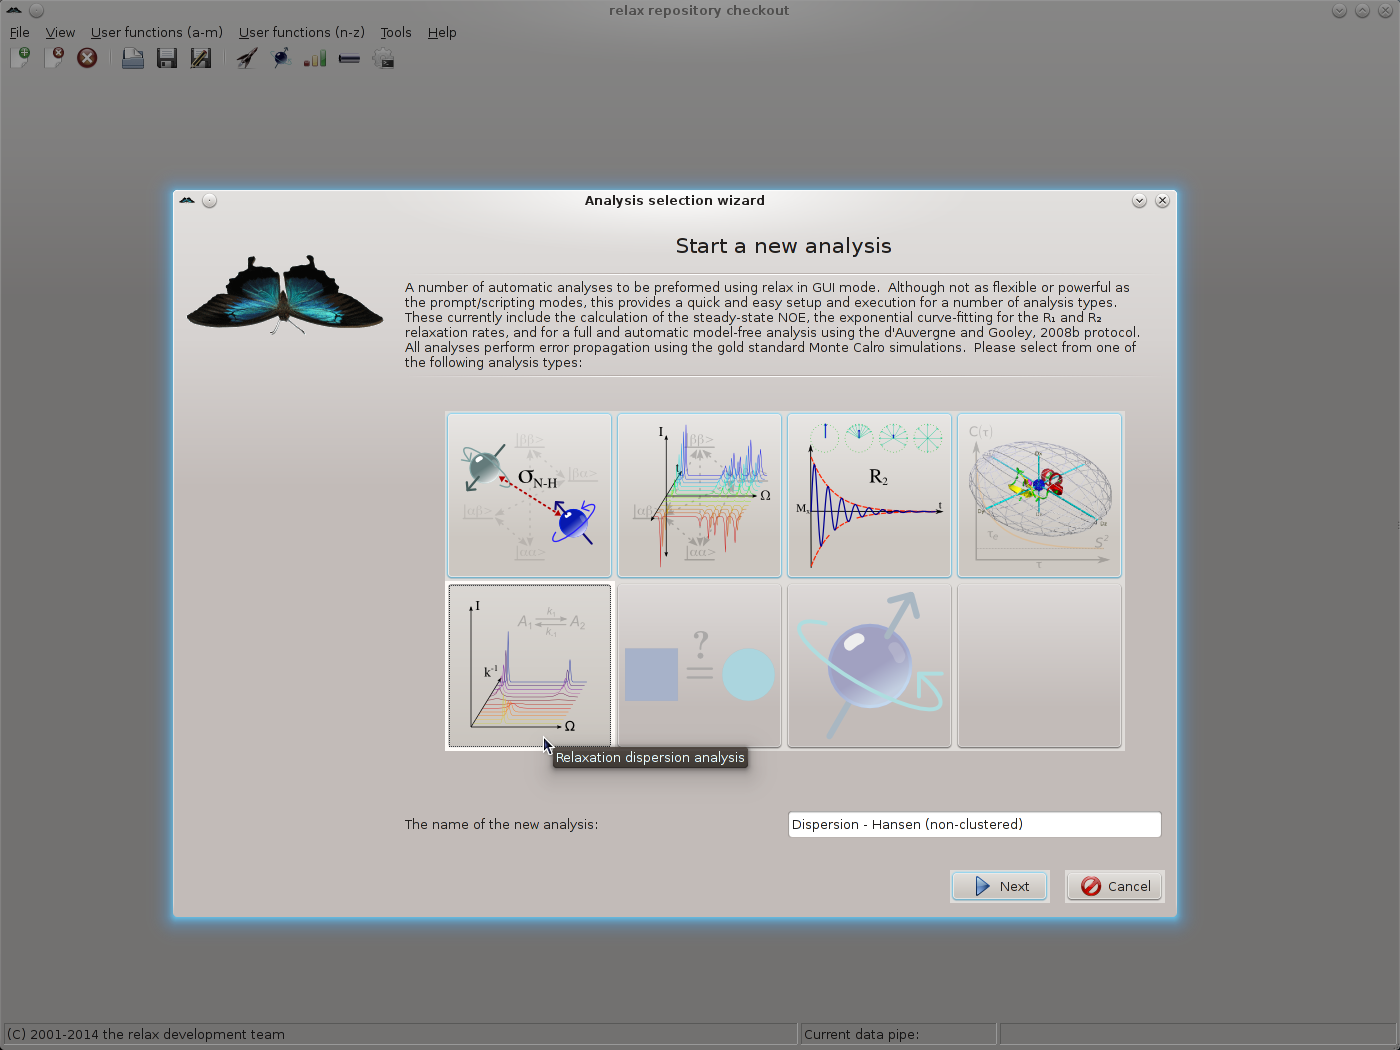
\includegraphics[
      width=0.9\textwidth,
      bb=14 14 1065 802
    ]
    {graphics/screenshots/dispersion_analysis/analysis_wizard1}
  }
\end{minipage}

Click on the \guibutton{Next} button to move to the second wizard page:

\begin{minipage}[h]{\linewidth}
  \centerline{
    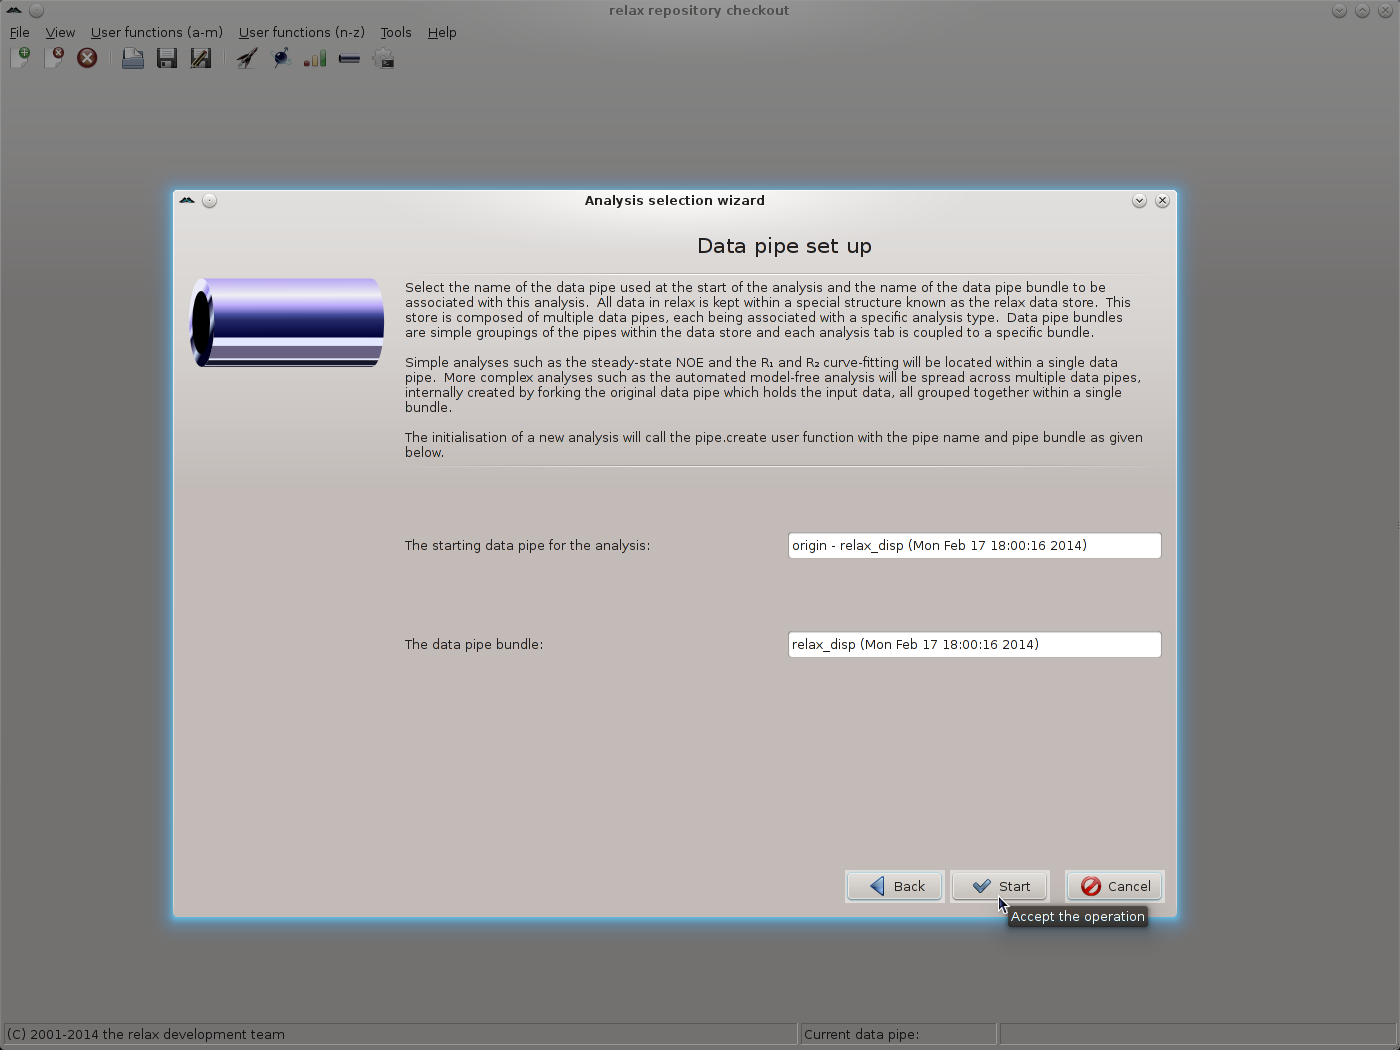
\includegraphics[
      width=0.9\textwidth,
      bb=14 14 1065 802
    ]
    {graphics/screenshots/dispersion_analysis/analysis_wizard2}
  }
\end{minipage}

Here the values need not be changed.
The data pipe bundle will be used to hold all the separate data pipes for each dispersion model type together.


% General setup.
%~~~~~~~~~~~~~~~

\subsection{Dispersion GUI mode -- general setup}

A blank analysis tab should now be visible:

\begin{minipage}[h]{\linewidth}
  \centerline{
    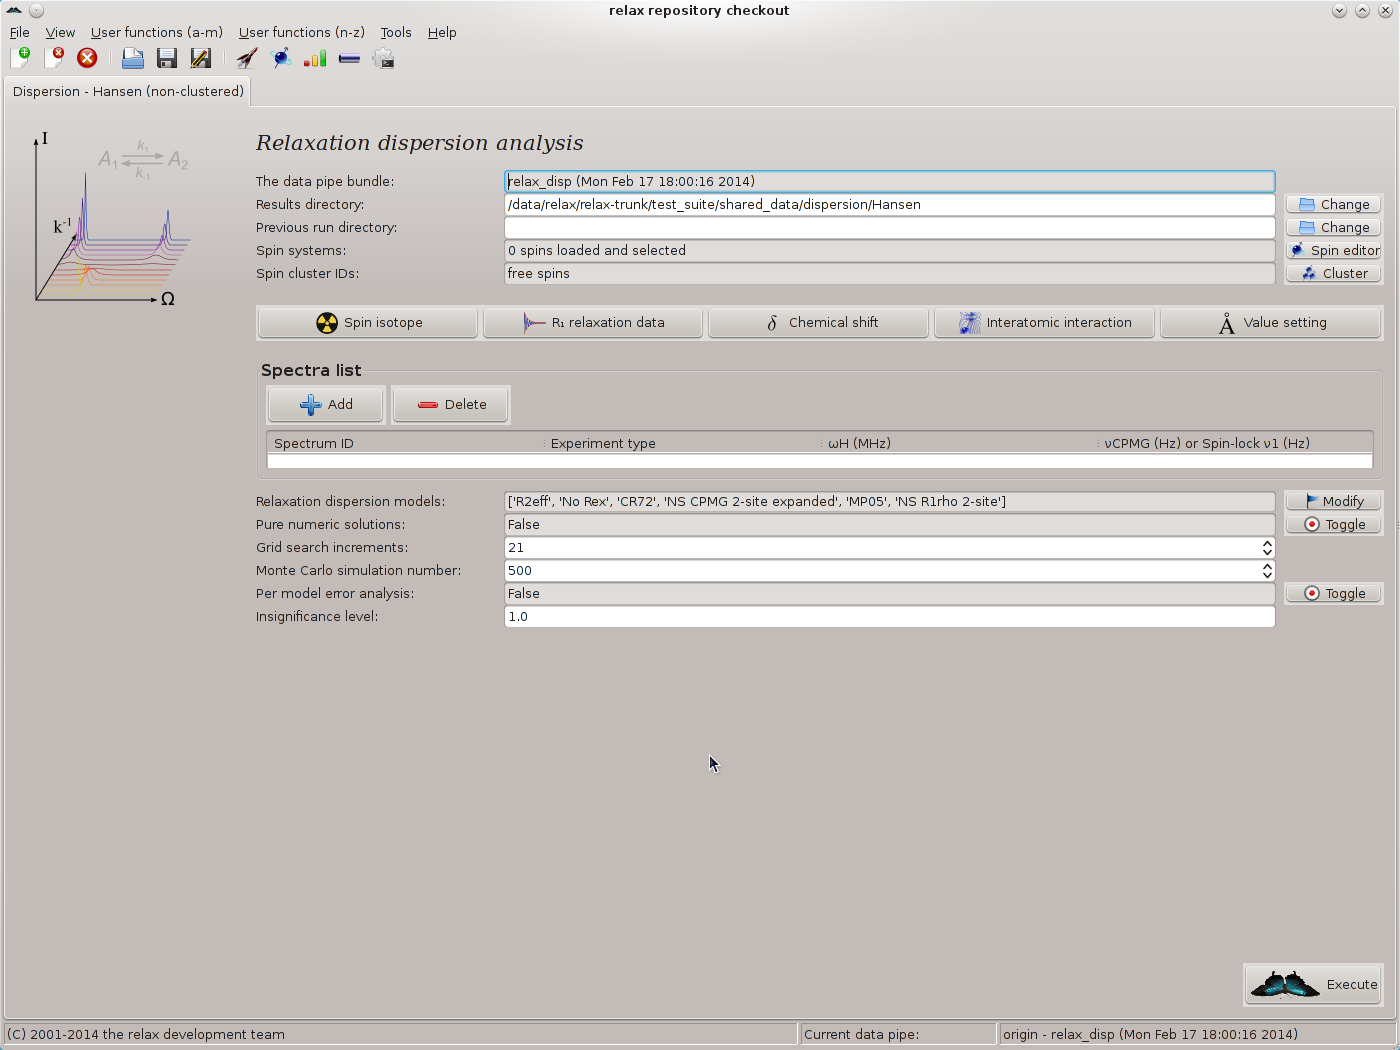
\includegraphics[
      width=0.9\textwidth,
      bb=14 14 1065 802
    ]
    {graphics/screenshots/dispersion_analysis/blank}
  }
\end{minipage}

The first step will be to change the \gui{Results directory} where all of the automatically created results file, 2D Grace plots, and relax state files will be saved.
The directory \directory{$\sim$\ossep{}tmp\ossep{}dispersion\ossep{}non\osus{}clustered} will be used for this initial non-clustered analysis.


% Spin systems.
%~~~~~~~~~~~~~~

\subsection{Dispersion GUI mode -- setting up the spin systems}

As the relaxation dispersion data is specific to individual nuclear spins, the molecule, residue and spin data structures need to be set up.
For this, the special \gui{Spin systems} GUI element can be used.
The initial state will be \gui{0 spins loaded and selected}.
Click on the \guibutton{Spin editor} button to launch the spin viewer window.
The steps for setting up the spin containers using PDB files are described in section~\ref{sect: GUI - structural data} on page~\pageref{sect: GUI - structural data} or for sequence files in section~\ref{sect: GUI - sequence file} on page~\pageref{sect: GUI - sequence file}.

In this tutorial, the sequence file \file{fake\osus{}sequence.in} in the \directory{test\osus{}suite\ossep{}shared\osus{}data\ossep{}dispersion\ossep{}Hansen} directory will be loaded.
In the spin loading wizard, which can be launched by clicking on the \guibutton{Load spins} button, select the \gui{From a file containing sequence data} option and click on \guibutton{Next}.
In the \uf{sequence\ufsep{}read} user function wizard page, select the \file{fake\osus{}sequence.in} file.
As this file only contains residue numbers and names (click on the \guibutton{preview} button to see the file contents), edit the \gui{Free format file settings} to set the residue number and name columns to 1 and 2 respectively and all other columns to blank values.
Click on \guibutton{Save} to store the free format settings and close the window.
Back in the \uf{sequence\ufsep{}read} user function wizard page, click on \guibutton{Next} to load the sequence.
Finally click on \guibutton{Finish} to close the wizard.
Do not close the spin viewer window yet.
Back in the main analysis tab, the \gui{Spin systems} GUI element will now say \gui{73 spins loaded and selected}.


% Unresolved spins.
%~~~~~~~~~~~~~~~~~~

\subsection{Dispersion GUI mode -- unresolved spins}

As in the prompt/script UI section~\ref{sect: dispersion setup fin}, the spins can be deselected at this point using the same \file{unresolved} files.
This is described in detail in section~\ref{sect: GUI - deselect spins} on page~\pageref{sect: GUI - deselect spins}.

Within the open spin viewer window, click on the \guimenuitemthree{User functions}{deselect}{read} menu item.
In the \uf{deselect\ufsep{}read} user function window, select the file \file{test\osus{}suite\ossep{}shared\osus{}data\ossep{}dispersion\ossep{}Hansen\ossep{}500\osus{}MHz\ossep{}unresolved}.
As this file only contains residue number, edit the \gui{Free format file settings} to set the residue number column to 1 and all other columns to empty values.
Click the \guibutton{Apply} button rather than \guibutton{OK} to allow a second file to be read.
The relax controller window may appear and can be closed.
Select the new file \file{test\osus{}suite\ossep{}shared\osus{}data\ossep{}dispersion\ossep{}Hansen\ossep{}800\osus{}MHz\ossep{}unresolved} and click on \guibutton{OK}.
Now all spins from these two files will be deselected and skipped in the analysis.


% Dispersion setup.
%~~~~~~~~~~~~~~~~~~

\subsection{Dispersion GUI mode -- dispersion setup}

The next step is to set up the data defining the relaxation dispersion process.
This is performed by clicking on the buttons between the \gui{Spin cluster ID} and \gui{Spectra list} GUI elements.
The buttons are as follows:
\begin{description}
  \item[Spin isotope:]  This is needed to specify the spin isotope information for each spin in the system, for example if the data is from $^{15}$N, $^{13}$C, $^1$H, etc.
    The button launches the \uf{spin.isotope} user function (see section~\ref{uf: spin.isotope} on page~\pageref{uf: spin.isotope}).
  \item[$\Rone$ relaxation data:]  This is used to load a text file containing $\Rone$ relaxation data for each spin of interest (see Chapter~\ref{ch: relax-fit} for calculating $\Rone$ values).
    The button launches the \uf{relax\_data.read} user function (see section~\ref{uf: relax_data.read} on page~\pageref{uf: relax_data.read}).
    It is currently only used for handling off-resonance effects in the $\Ronerho$-type dispersion data but may be extended, in the future, to handle off-resonance effects in the CPMG-type experiments.
  \item[Chemical shift:]  As with the $\Rone$ button, this is for properly handling off-resonance effects in the $\Ronerho$-type dispersion data.
    The button launches the \uf{chemical\_shift.read} user function (see section~\ref{uf: chemical_shift.read} on page~\pageref{uf: chemical_shift.read}).
  \item[Interatomic interaction:]  This button launches the \uf{interatom.define} user function (see section~\ref{uf: interatom.define} on page~\pageref{uf: interatom.define}).
    This is needed to link, for example, $^1$H to $^{15}$N spins into a spin system so that MMQ-type data, which relies on a multiple-spin system, can be handled.
  \item[Value setting:]  When one of the parameters of the dispersion model is already known, its value can be set by clicking on this button which launches the \uf{value.set} user function (see section~\ref{uf: value.set} on page~\pageref{uf: value.set}).
    Setting a parameter value will fix the parameter in the initial grid search.
    However it will be free to vary in the non-linear least squares optimisation used to refine its value.
\end{description}

For SQ CPMG-type dispersion data, only the spin isotope information is required:

\begin{minipage}[h]{\linewidth}
  \centerline{
    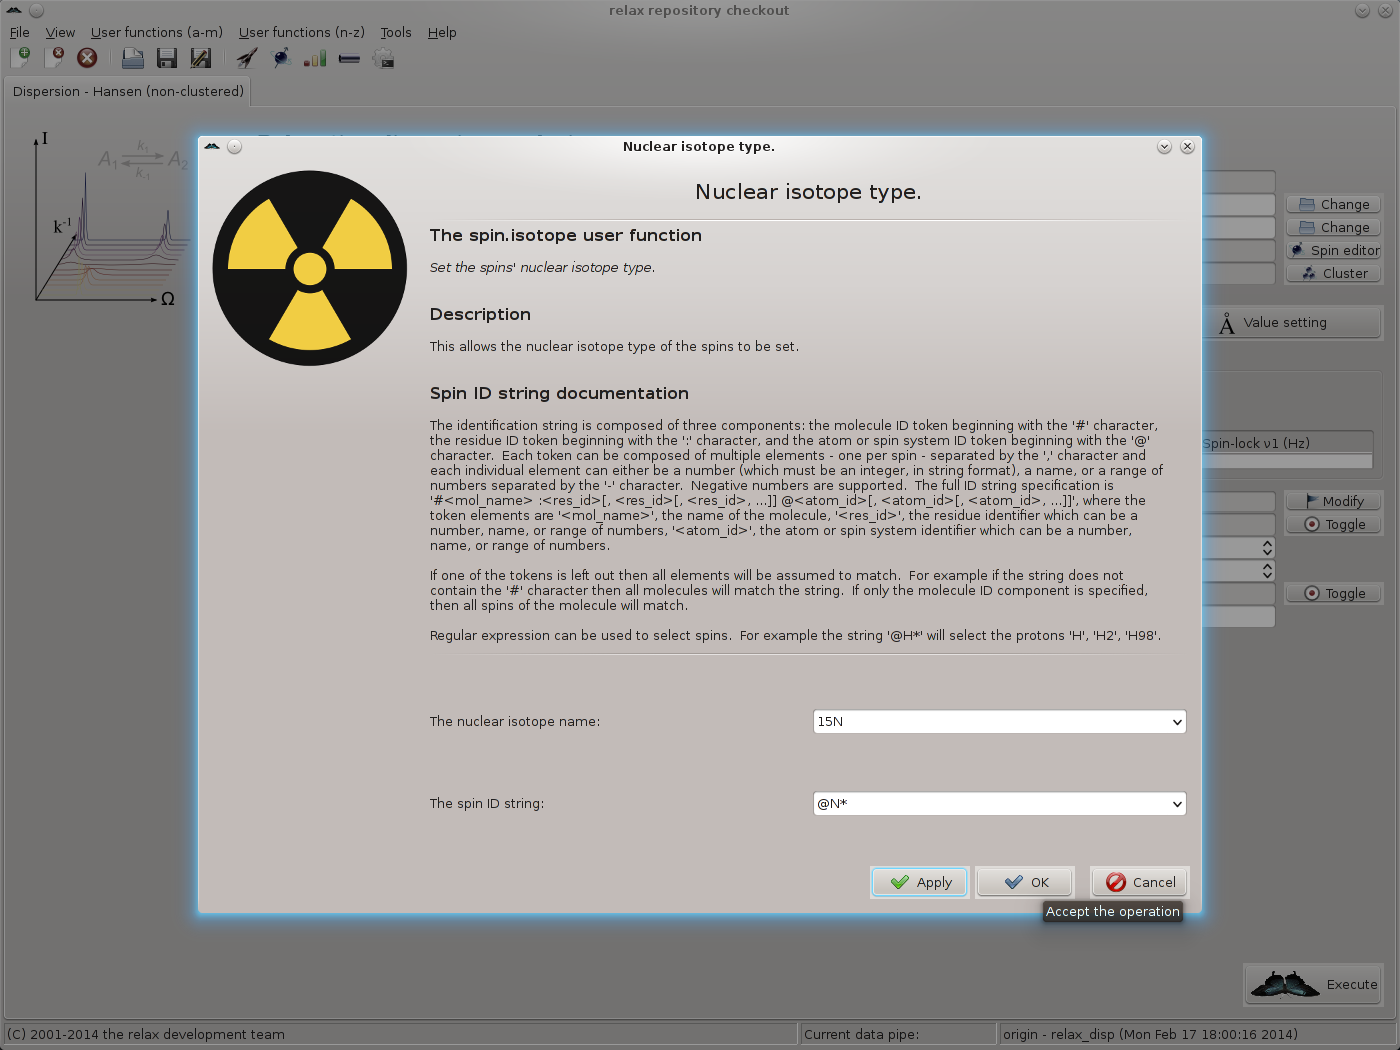
\includegraphics[
      width=0.9\textwidth,
      bb=14 14 1065 802
    ]
    {graphics/screenshots/dispersion_analysis/spin_isotope}
  }
\end{minipage}

In this case, all spins are $^{15}$N.
However as no spins are named yet, the text \guistring{@N*} cannot be used.
So simply change this to \guistring{@*} and click on \guibutton{OK}.
The other buttons can be ignored.


% Loading the data.
%~~~~~~~~~~~~~~~~~~

\subsection{Dispersion GUI mode -- loading the data}

The standard way for handling experimental NMR data for starting a relaxation dispersion analysis in the relax GUI is to load the peak intensity values (either height or volume) from a peak list.
For a list of all the currently supported peak list formats, see the \uf{spectrum\ufsep{}read\ufus{}intensities} user function documentation in section~\ref{uf: spectrum.read_intensities} on page~\pageref{uf: spectrum.read_intensities}.

Note that relax also accepts pre-fitted or pre-calculated $\Rtwoeff$ or $\Ronerho$ values via the \uf{relax\ufus{}disp\ufsep{}r2eff\ufus{}read} and \uf{relax\ufus{}disp\ufsep{}r2eff\ufus{}read\ufus{}spin} user functions (see section~\ref{uf: relax_disp.r2eff_read} on page~\pageref{uf: relax_disp.r2eff_read} and section~\ref{uf: relax_disp.r2eff_read_spin} on page~\pageref{uf: relax_disp.r2eff_read_spin} respectively), however this is not the standard way of using the GUI.
As this is not tested, if you decide to work with pre-calculated relaxation rates please report any bugs encountered as described in section~\ref{reporting bugs} on page~\pageref{reporting bugs}.
To access the user functions, click on \guimenuitemthree{User functions}{relax\_disp}{r2eff\_read} or \guimenuitemthree{User functions}{relax\_disp}{r2eff\_read\_spin}.

In this tutorial, the Sparky\index{software!Sparky} formatted peak lists in the \directory{test\osus{}suite\ossep{}shared\osus{}data\ossep{}dispersion\ossep{}Hansen\ossep{}500\osus{}MHz} and \directory{test\osus{}suite\ossep{}shared\osus{}data\ossep{}dispersion\ossep{}Hansen\ossep{}800\osus{}MHz} directories will be loaded.
First click on the \guibutton{Add} button in the \gui{Spectra list} GUI element.
A warning message will appear as the spins have not yet been named, spin names were not present in the \file{fake\osus{}sequence.in} file, hence they cannot be matched to the data in the peak lists:

\begin{minipage}[h]{\linewidth}
  \centerline{
    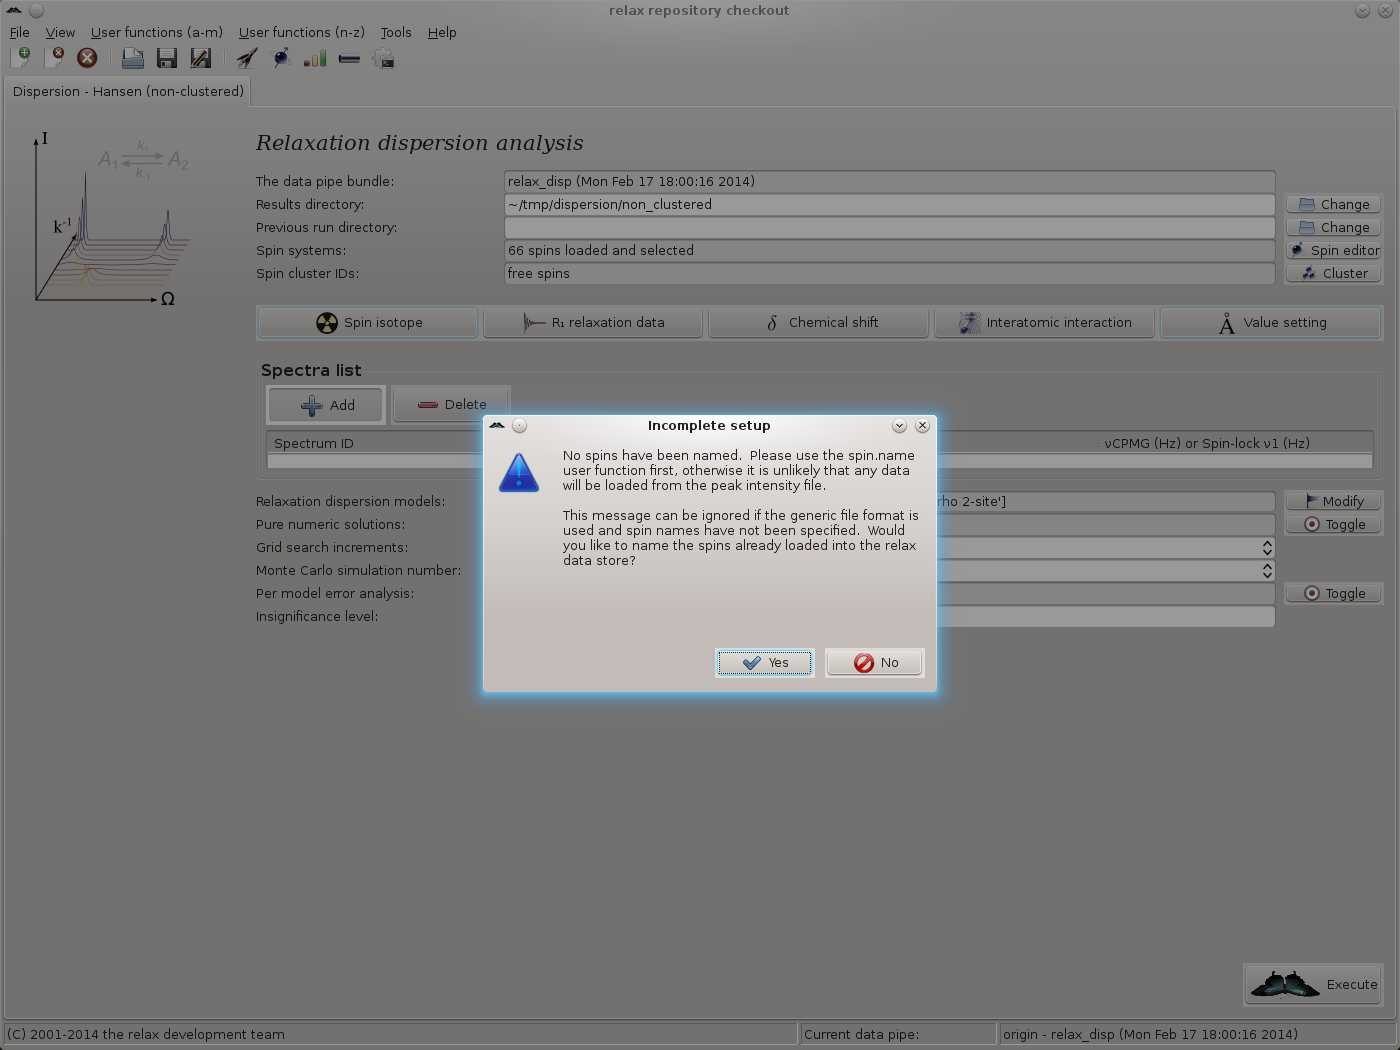
\includegraphics[
      width=0.9\textwidth,
      bb=14 14 1065 802
    ]
    {graphics/screenshots/dispersion_analysis/spectrum_incomplete_setup}
  }
\end{minipage}

Simply click on \guibutton{Yes} to allow the spins to be named in the next step.
The \uf{spin\ufsep{}name} user function wizard page should now appear.
As all data is from $^{15}$N spins and these spins have been named as \guistring{N} in the Sparky peak lists, set the new spin name to \guistring{N} and click on \guibutton{Next}:

\begin{minipage}[h]{\linewidth}
  \centerline{
    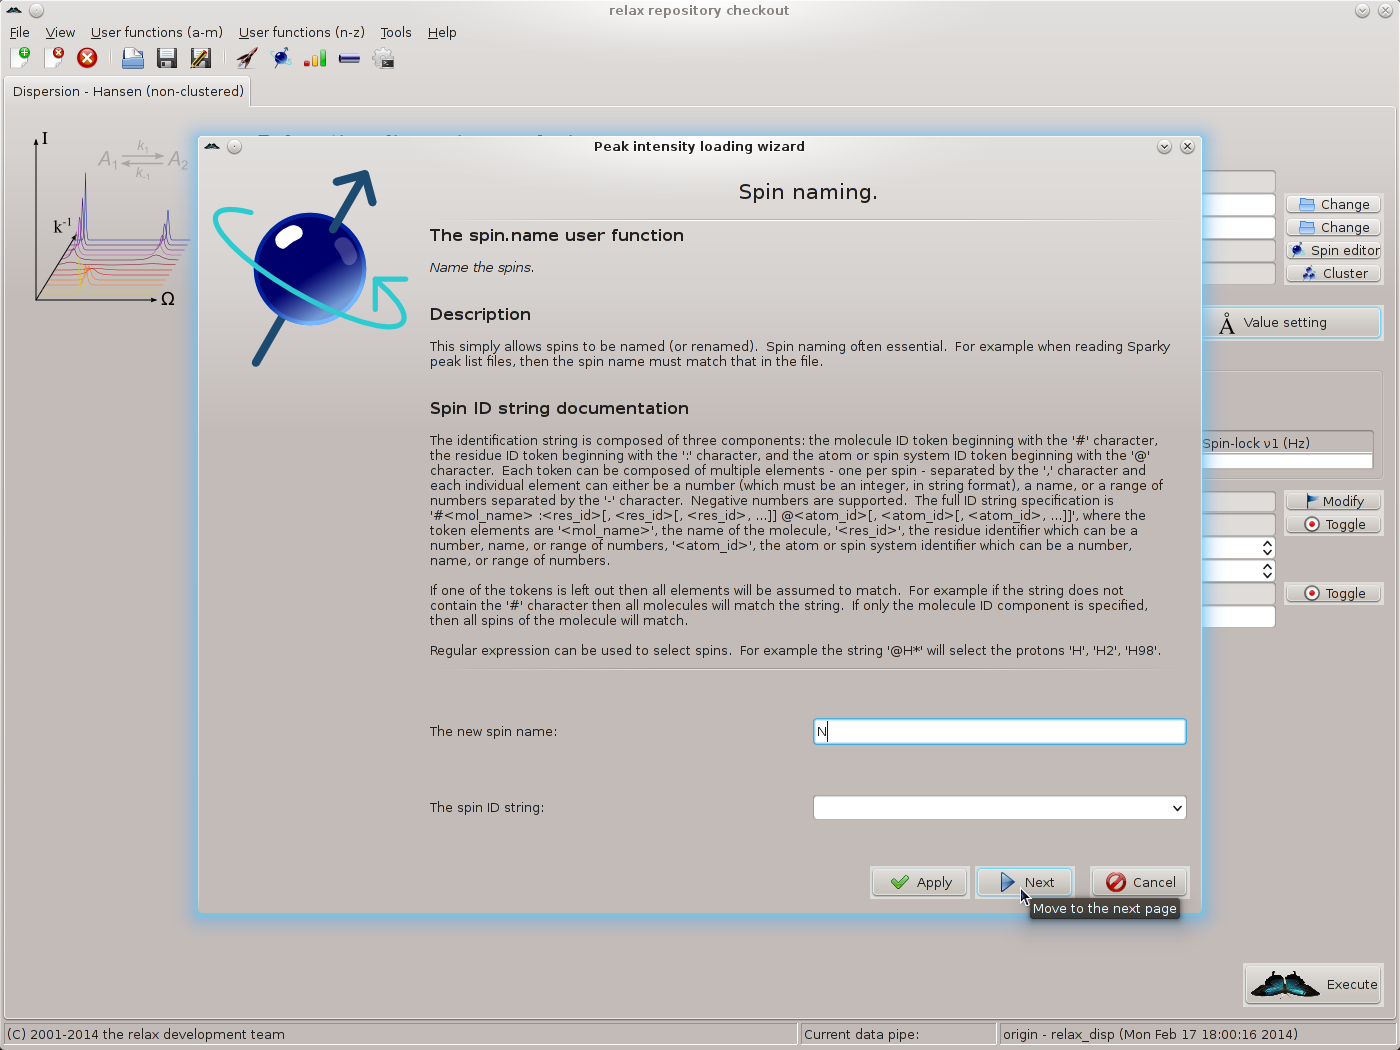
\includegraphics[
      width=0.9\textwidth,
      bb=14 14 1065 802
    ]
    {graphics/screenshots/dispersion_analysis/spectrum_spin_name}
  }
\end{minipage}

The \uf{spectrum\ufsep{}read\ufus{}intensities} user function wizard page should appear.
To help understand the next steps of the peak intensity loading wizard, note the following table which summarises the peak list metadata for this analysis:

\begin{center}        
\begin{footnotesize}
\begin{tabular}{llllll}
\toprule

File name   & Spectrum ID & Spectrometer & $\nucpmg$ & Replicate \\
            &             & frq. (MHz)   & (Hz)      & IDs       \\

\midrule

\file{500\osus{}MHz\ossep{}reference.in\osus{}sparky}   & 500\_ref      &  500.0  &       None   &              \\
\file{500\osus{}MHz\ossep{}66.667.in\osus{}sparky}      & 500\_66.667   &  500.0  &    66.6666   &              \\
\file{500\osus{}MHz\ossep{}133.33.in\osus{}sparky}      & 500\_133.33   &  500.0  &   133.3333   & 500\_133.33b \\
\file{500\osus{}MHz\ossep{}133.33.in.bis\osus{}sparky}  & 500\_133.33b  &  500.0  &   133.3333   & 500\_133.33  \\
\file{500\osus{}MHz\ossep{}200.in\osus{}sparky}         & 500\_200.00   &  500.0  &   200.0000   &              \\
\file{500\osus{}MHz\ossep{}266.67.in\osus{}sparky}      & 500\_266.67   &  500.0  &   266.6666   &              \\
\file{500\osus{}MHz\ossep{}333.33.in\osus{}sparky}      & 500\_333.33   &  500.0  &   333.3333   &              \\
\file{500\osus{}MHz\ossep{}400.in\osus{}sparky}         & 500\_400.00   &  500.0  &   400.0000   &              \\
\file{500\osus{}MHz\ossep{}466.67.in\osus{}sparky}      & 500\_466.67   &  500.0  &   466.6666   &              \\
\file{500\osus{}MHz\ossep{}533.33.in\osus{}sparky}      & 500\_533.33   &  500.0  &   533.3333   & 500\_533.33b \\
\file{500\osus{}MHz\ossep{}533.33.in.bis\osus{}sparky}  & 500\_533.33b  &  500.0  &   533.3333   & 500\_533.33  \\
\file{500\osus{}MHz\ossep{}600.in\osus{}sparky}         & 500\_600.00   &  500.0  &   600.0000   &              \\
\file{500\osus{}MHz\ossep{}666.67.in\osus{}sparky}      & 500\_666.67   &  500.0  &   666.6666   &              \\
\file{500\osus{}MHz\ossep{}733.33.in\osus{}sparky}      & 500\_733.33   &  500.0  &   733.3333   &              \\
\file{500\osus{}MHz\ossep{}800.in\osus{}sparky}         & 500\_800.00   &  500.0  &   800.0000   &              \\
\file{500\osus{}MHz\ossep{}866.67.in\osus{}sparky}      & 500\_866.67   &  500.0  &   866.6666   &              \\
\file{500\osus{}MHz\ossep{}933.33.in\osus{}sparky}      & 500\_933.33   &  500.0  &   933.3333   & 500\_933.33b \\
\file{500\osus{}MHz\ossep{}933.33.in.bis\osus{}sparky}  & 500\_933.33b  &  500.0  &   933.3333   & 500\_933.33  \\
\file{500\osus{}MHz\ossep{}1000.in\osus{}sparky}        & 500\_1000.0   &  500.0  &  1000.0000   &              \\
 \\
\file{800\osus{}MHz\ossep{}reference.in\osus{}sparky}   & 800\_ref      &  800.0  &       None   &              \\
\file{800\osus{}MHz\ossep{}66.667.in\osus{}sparky}      & 800\_66.667   &  800.0  &    66.6666   &              \\
\file{800\osus{}MHz\ossep{}133.33.in\osus{}sparky}      & 800\_133.33   &  800.0  &   133.3333   & 800\_133.33b \\
\file{800\osus{}MHz\ossep{}133.33.in.bis\osus{}sparky}  & 800\_133.33b  &  800.0  &   133.3333   & 800\_133.33  \\
\file{800\osus{}MHz\ossep{}200.in\osus{}sparky}         & 800\_200.00   &  800.0  &   200.0000   &              \\
\file{800\osus{}MHz\ossep{}266.67.in\osus{}sparky}      & 800\_266.67   &  800.0  &   266.6666   &              \\
\file{800\osus{}MHz\ossep{}333.33.in\osus{}sparky}      & 800\_333.33   &  800.0  &   333.3333   &              \\
\file{800\osus{}MHz\ossep{}400.in\osus{}sparky}         & 800\_400.00   &  800.0  &   400.0000   &              \\
\file{800\osus{}MHz\ossep{}466.67.in\osus{}sparky}      & 800\_466.67   &  800.0  &   466.6666   &              \\
\file{800\osus{}MHz\ossep{}533.33.in\osus{}sparky}      & 800\_533.33   &  800.0  &   533.3333   & 800\_533.33b \\
\file{800\osus{}MHz\ossep{}533.33.in.bis\osus{}sparky}  & 800\_533.33b  &  800.0  &   533.3333   & 800\_533.33  \\
\file{800\osus{}MHz\ossep{}600.in\osus{}sparky}         & 800\_600.00   &  800.0  &   600.0000   &              \\
\file{800\osus{}MHz\ossep{}666.67.in\osus{}sparky}      & 800\_666.67   &  800.0  &   666.6666   &              \\
\file{800\osus{}MHz\ossep{}733.33.in\osus{}sparky}      & 800\_733.33   &  800.0  &   733.3333   &              \\
\file{800\osus{}MHz\ossep{}800.in\osus{}sparky}         & 800\_800.00   &  800.0  &   800.0000   &              \\
\file{800\osus{}MHz\ossep{}866.67.in\osus{}sparky}      & 800\_866.67   &  800.0  &   866.6666   &              \\
\file{800\osus{}MHz\ossep{}933.33.in\osus{}sparky}      & 800\_933.33   &  800.0  &   933.3333   & 800\_933.33b \\
\file{800\osus{}MHz\ossep{}933.33.in.bis\osus{}sparky}  & 800\_933.33b  &  800.0  &   933.3333   & 800\_933.33  \\
\file{800\osus{}MHz\ossep{}1000.in\osus{}sparky}        & 800\_1000.0   &  800.0  &  1000.0000   &              \\

\bottomrule
\end{tabular}
\end{footnotesize}
\end{center}

For all of these files, the experiment type is SQ CPMG and the relaxation delay time is 30~ms.
All files are located in the \directory{test\osus{}suite\ossep{}shared\osus{}data\ossep{}dispersion\ossep{}Hansen} base directory.

To simplify the loading of the data, all of the 500 MHz data will be read simultaneously (followed by all of the 800 MHz data).
Firstly, to select all of the 500~MHz files, click on the button at the end of the \guistring{file name(s)} GUI element.
This will launch the multiple file selection window:

\begin{minipage}[h]{\linewidth}
  \centerline{
    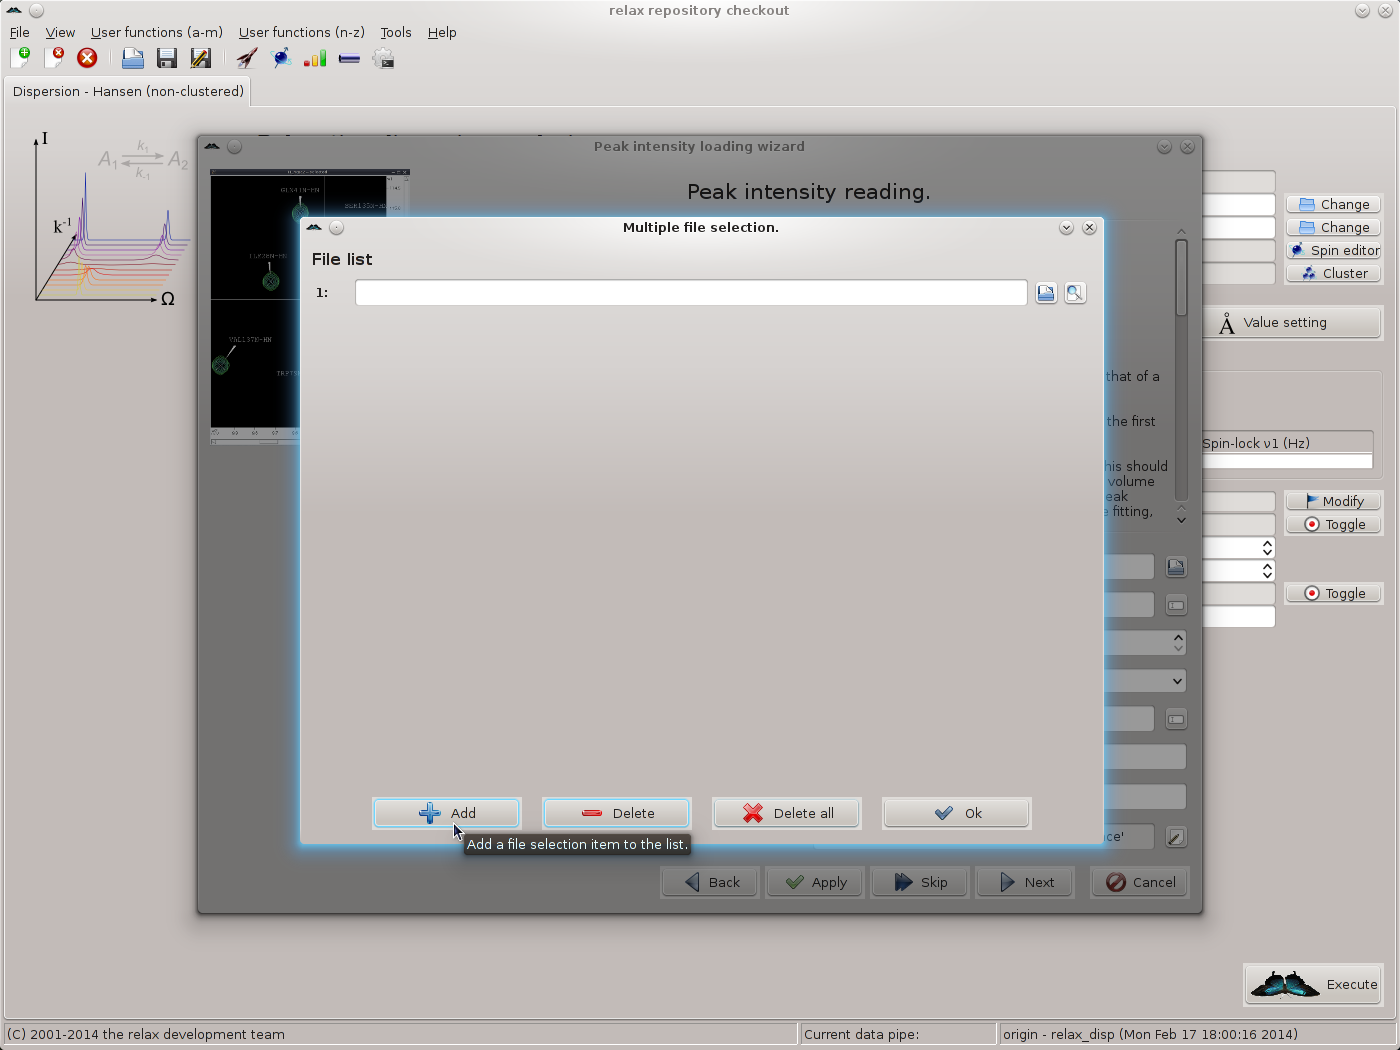
\includegraphics[
      width=0.9\textwidth,
      bb=14 14 1415 1065
    ]
    {graphics/screenshots/dispersion_analysis/spectrum_file_selection}
  }
\end{minipage}

Add the first file by typing the file name or clicking on the file selection button to the right of the file input field and choosing the file.
A preview button is included to allow the file to be checked.
Then click on the \guibutton{Add} button to insert a new file selection item, add the next file, and continue until completion.
You should now see 19 file names:

\begin{minipage}[h]{\linewidth}
  \centerline{
    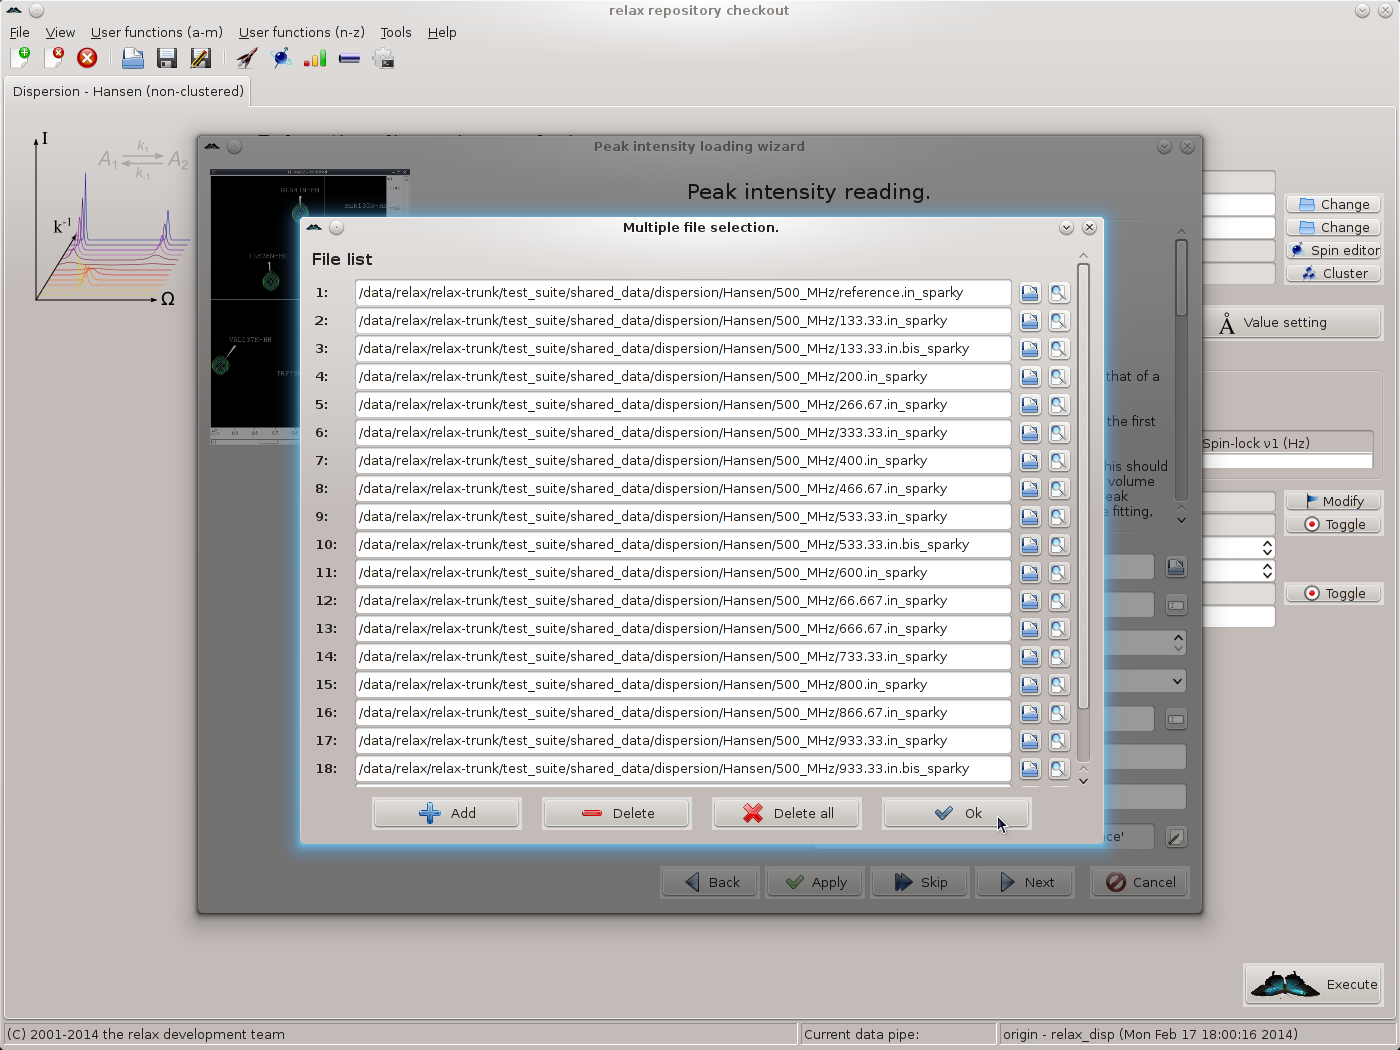
\includegraphics[
      width=0.9\textwidth,
      bb=14 14 1415 1065
    ]
    {graphics/screenshots/dispersion_analysis/spectrum_file_selection_fin}
  }
\end{minipage}

Click on \guibutton{OK} to return to the \uf{spectrum\ufsep{}read\ufus{}intensities} user function wizard page.
Next, the spectrum IDs should be set.
For this, click on the button to the far right of the \guistring{spectrum ID string} GUI element.
Click on \guibutton{Add} and fill in the spectrum IDs corresponding to the files selected.
As 19 files exist for the 500 MHz data, 19 spectrum IDs should be added.
When complete you should see:

\begin{minipage}[h]{\linewidth}
  \centerline{
    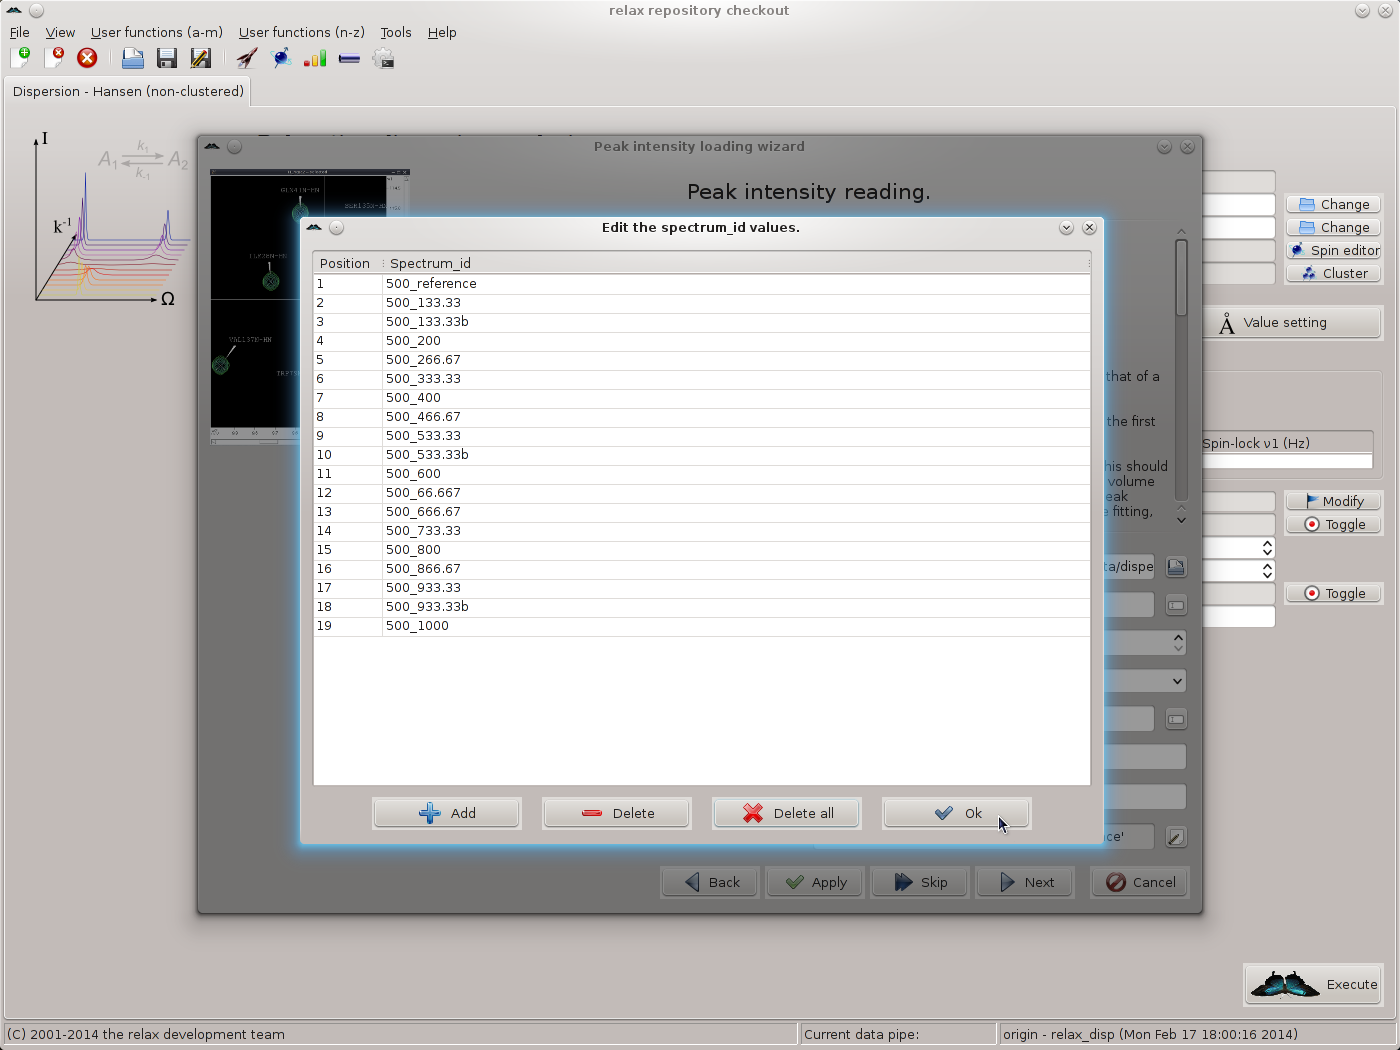
\includegraphics[
      width=0.9\textwidth,
      bb=14 14 1415 1065
    ]
    {graphics/screenshots/dispersion_analysis/spectrum_spectrum_ids}
  }
\end{minipage}

Click on \guibutton{OK} to return to the \uf{spectrum\ufsep{}read\ufus{}intensities} user function wizard page.

There is a shortcut to these previous steps in that the file names and spectrum IDs can be manually typed into the input elements of the \uf{spectrum\ufsep{}read\ufus{}intensities} user function wizard page.
For the file names, assuming relax is installed in the base directory \directory{\ossep{}data\ossep{}relax\ossep{}relax-trunk} and a Unix-like system is being used, the following text can be added:

\begin{lstlisting}[numbers=none]
['/data/relax/relax-trunk/test_suite/shared_data/dispersion/Hansen/500_MHz/reference.in_sparky', '/data/relax/relax-trunk/test_suite/shared_data/dispersion/Hansen/500_MHz/133.33.in_sparky', '/data/relax/relax-trunk/test_suite/shared_data/dispersion/Hansen/500_MHz/133.33.in.bis_sparky', '/data/relax/relax-trunk/test_suite/shared_data/dispersion/Hansen/500_MHz/200.in_sparky', '/data/relax/relax-trunk/test_suite/shared_data/dispersion/Hansen/500_MHz/266.67.in_sparky', '/data/relax/relax-trunk/test_suite/shared_data/dispersion/Hansen/500_MHz/333.33.in_sparky', '/data/relax/relax-trunk/test_suite/shared_data/dispersion/Hansen/500_MHz/400.in_sparky', '/data/relax/relax-trunk/test_suite/shared_data/dispersion/Hansen/500_MHz/466.67.in_sparky', '/data/relax/relax-trunk/test_suite/shared_data/dispersion/Hansen/500_MHz/533.33.in_sparky', '/data/relax/relax-trunk/test_suite/shared_data/dispersion/Hansen/500_MHz/533.33.in.bis_sparky', '/data/relax/relax-trunk/test_suite/shared_data/dispersion/Hansen/500_MHz/600.in_sparky', '/data/relax/relax-trunk/test_suite/shared_data/dispersion/Hansen/500_MHz/66.667.in_sparky', '/data/relax/relax-trunk/test_suite/shared_data/dispersion/Hansen/500_MHz/666.67.in_sparky', '/data/relax/relax-trunk/test_suite/shared_data/dispersion/Hansen/500_MHz/733.33.in_sparky', '/data/relax/relax-trunk/test_suite/shared_data/dispersion/Hansen/500_MHz/800.in_sparky', '/data/relax/relax-trunk/test_suite/shared_data/dispersion/Hansen/500_MHz/866.67.in_sparky', '/data/relax/relax-trunk/test_suite/shared_data/dispersion/Hansen/500_MHz/933.33.in_sparky', '/data/relax/relax-trunk/test_suite/shared_data/dispersion/Hansen/500_MHz/933.33.in.bis_sparky', '/data/relax/relax-trunk/test_suite/shared_data/dispersion/Hansen/500_MHz/1000.in_sparky']
\end{lstlisting}

The spectrum IDs can be added by copying and pasting the following text, making sure all text is on one line:

\begin{lstlisting}[numbers=none]
['500_reference', '500_133.33', '500_133.33b', '500_200', '500_266.67', '500_333.33', '500_400', '500_466.67', '500_533.33', '500_533.33b', '500_600', '500_66.667', '500_666.67', '500_733.33', '500_800', '500_866.67', '500_933.33', '500_933.33b', '500_1000']
\end{lstlisting}

To see if the data has been correctly entered, click on the buttons to the right of the GUI elements.
You should see the files and spectrum IDs correctly listed in the multiple file selection window and the sequence input window respectively.

For the SQ CPMG data of this tutorial, none of the other settings in the \uf{spectrum\ufsep{}read\ufus{}intensities} user function wizard page need to be changed.
By clicking on the \guibutton{Apply} button, the 500 MHz data will be loaded but the wizard will stay on the same page.
Note that the contents of the main relax window will have changed.
Clicking \guibutton{Apply} rather than \guibutton{Next} will allow the 800 MHz data to be loaded next.
Change all of the file names and spectrum IDs for the 800 MHz and click on the \guibutton{Next} button to read the data and to move to the next wizard page.
This will be the page for specifying the types of errors to use:

\begin{minipage}[h]{\linewidth}
  \centerline{
    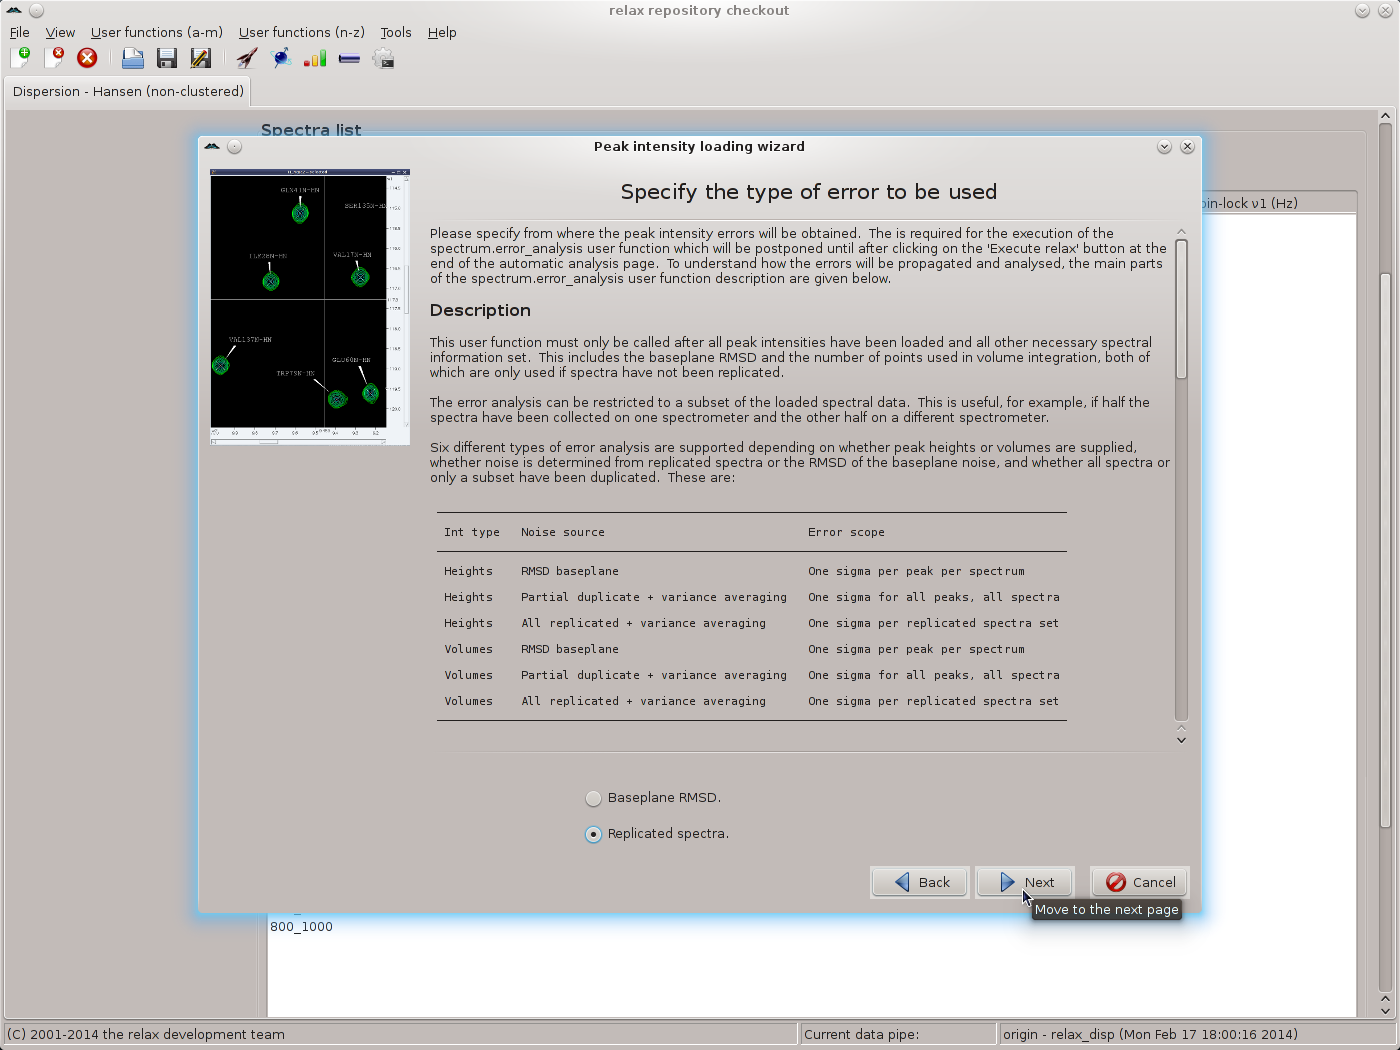
\includegraphics[
      width=0.9\textwidth,
      bb=14 14 1415 1065
    ]
    {graphics/screenshots/dispersion_analysis/spectrum_error_type}
  }
\end{minipage}

As replicated spectra have been collected, set the value to \guistring{Replicated spectra} and then click the \guibutton{Next} button.
Select the pairs of spectra which have been replicated and click the \guibutton{Apply} button to allow all of the replicates to be specified:

\begin{minipage}[h]{\linewidth}
  \centerline{
    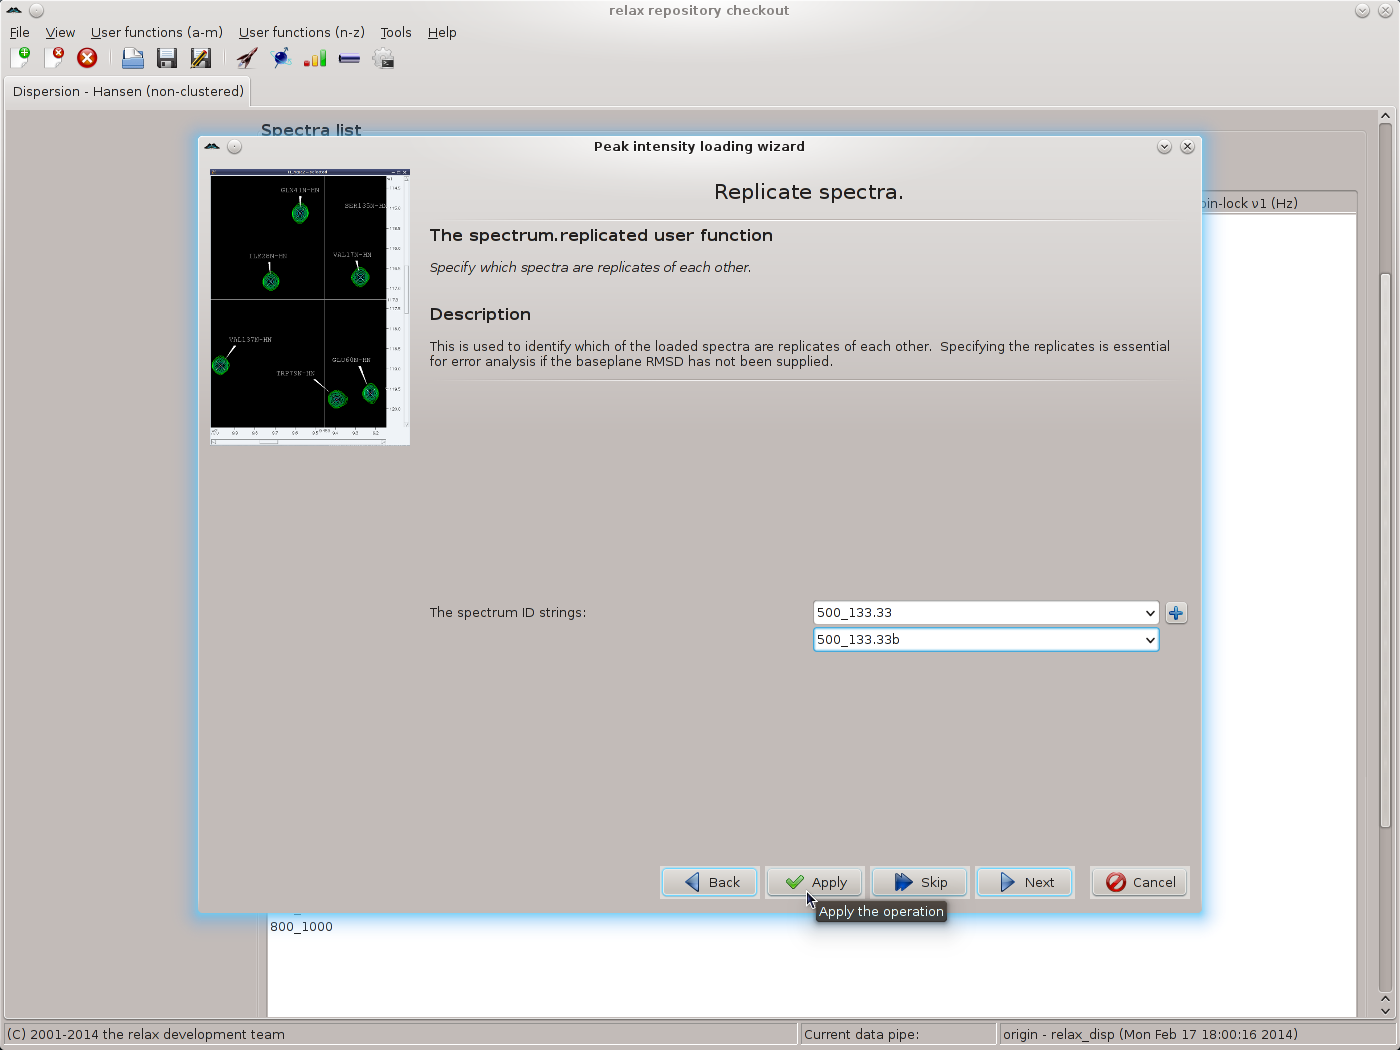
\includegraphics[
      width=0.9\textwidth,
      bb=14 14 1415 1065
    ]
    {graphics/screenshots/dispersion_analysis/spectrum_replicates}
  }
\end{minipage}

Repeat for each pair of replicates, then click the \guibutton{Next} button to move to the next wizard page -- the \uf{relax\ufus{}disp\ufsep{}exp\ufus{}type} user function.
Here the tedious operation of labelling all spectrum IDs as being \guistring{Single quantum (SQ) CPMG-type data} must be performed.
Select the spectrum ID and the SQ CPMG data type and click on the \guibutton{Apply} button, repeating for each ID:

\begin{minipage}[h]{\linewidth}
  \centerline{
    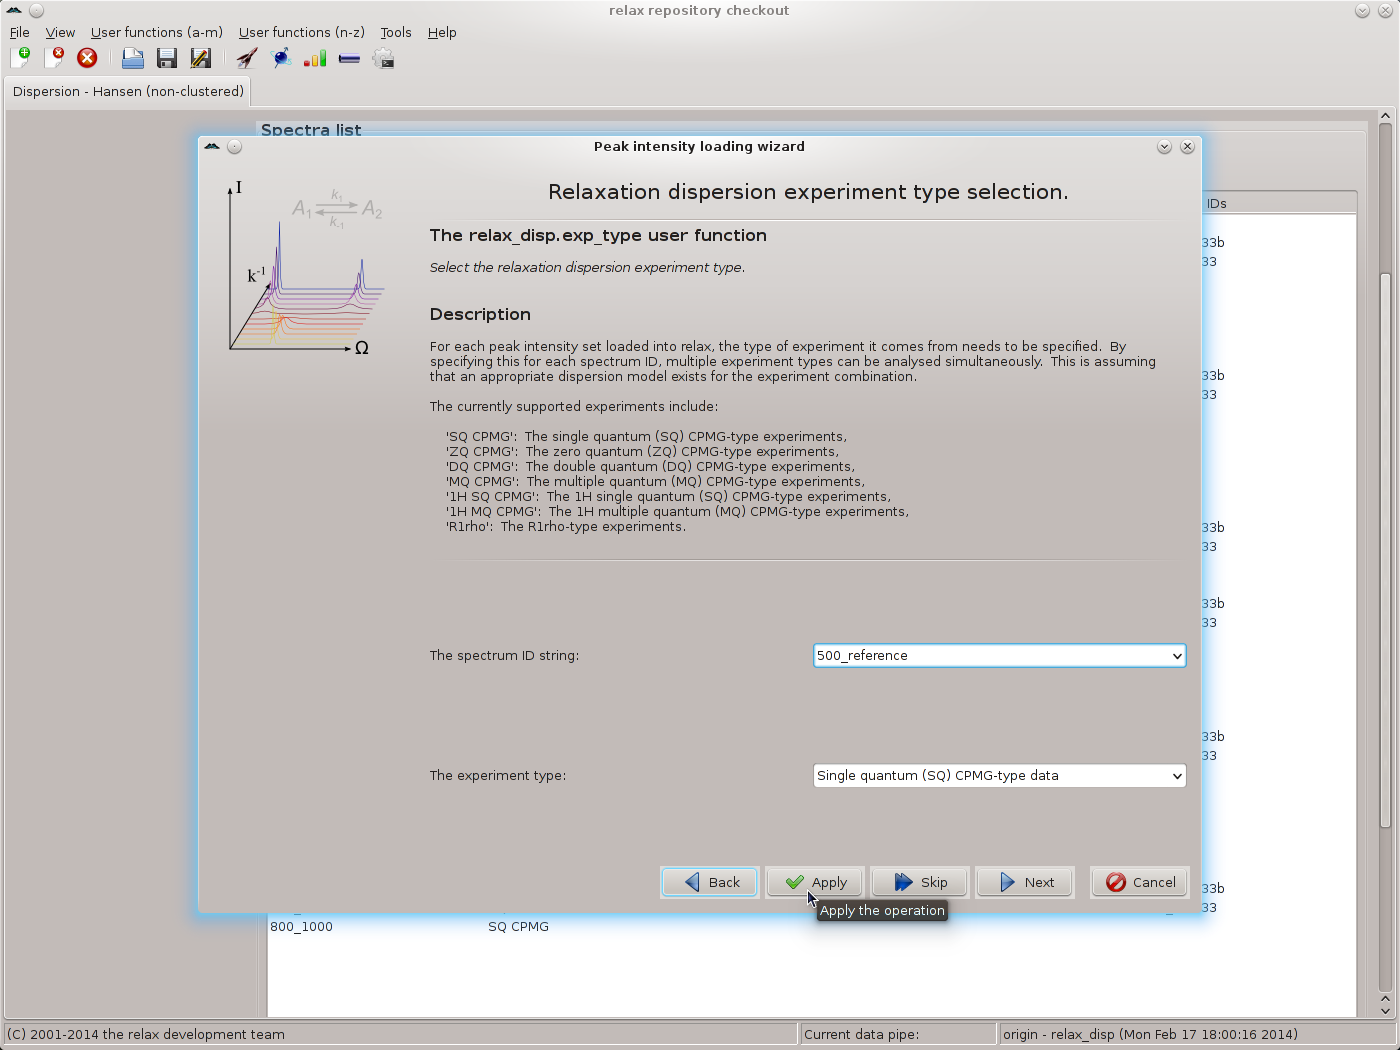
\includegraphics[
      width=0.9\textwidth,
      bb=14 14 1415 1065
    ]
    {graphics/screenshots/dispersion_analysis/spectrum_exp_type}
  }
\end{minipage}

Click the \guibutton{Next} button when finished.
The next wizard page will be that of the \uf{spectrometer\ufsep{}frequency} user function.
Here the exact spectrometer frequency values should be specified.
These values should be those of the \promptstring{sfrq} parameter in the Varian \file{procpar} file or the \promptstring{SFO1} parameter in the Bruker \file{acqus} file.
As the exact values are not known for the data of this tutorial, the values of 500.0 and 800.0 MHz will be used:

\begin{minipage}[h]{\linewidth}
  \centerline{
    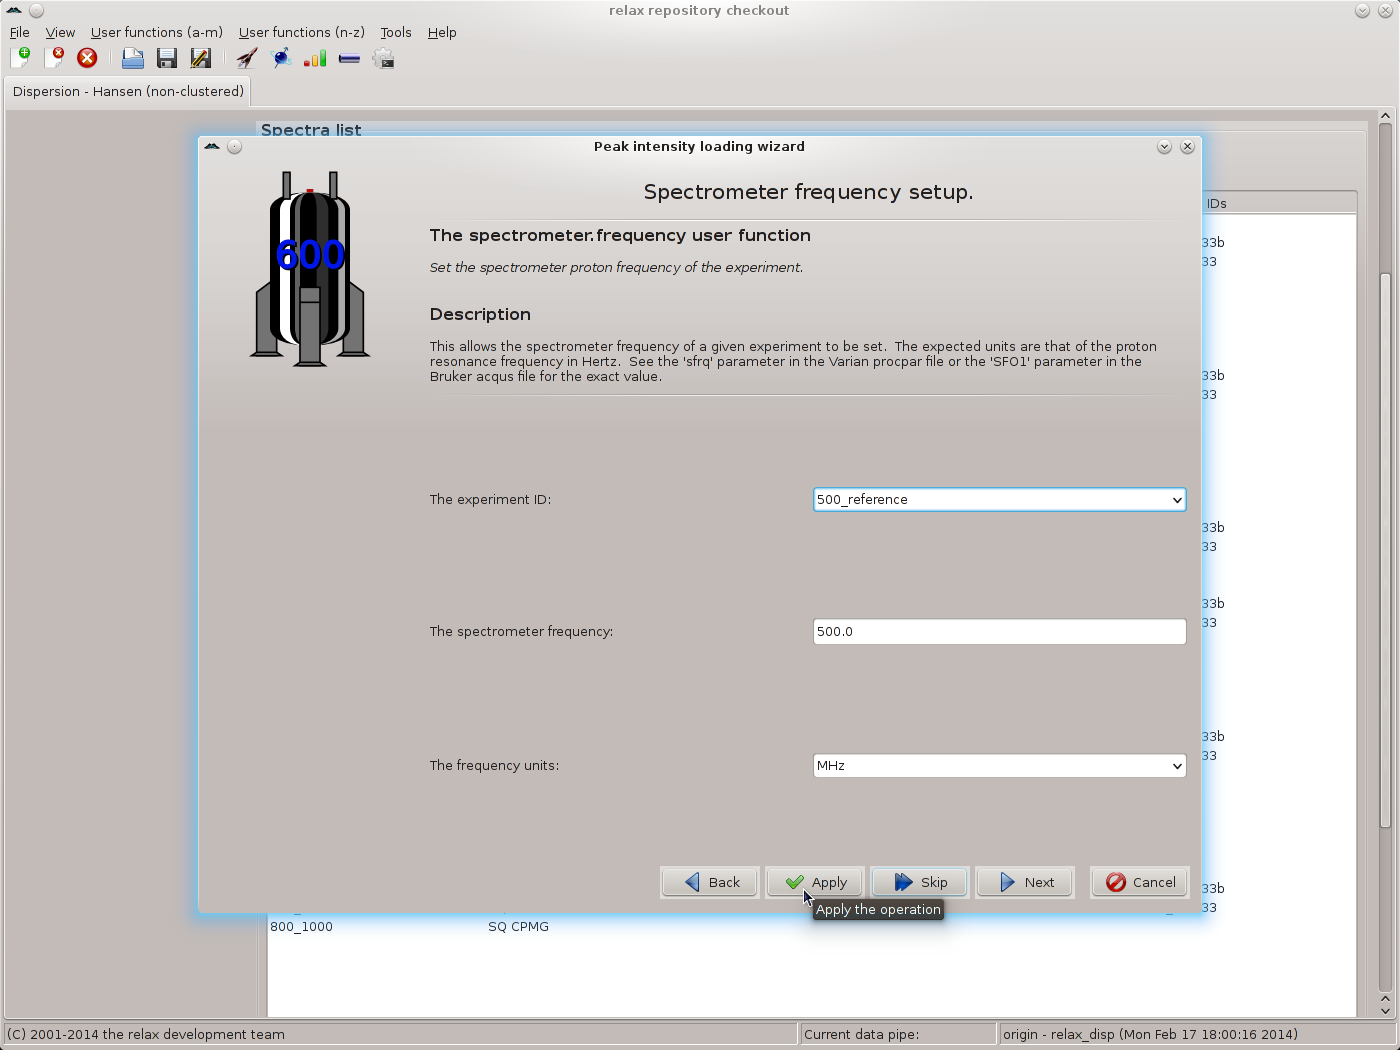
\includegraphics[
      width=0.9\textwidth,
      bb=14 14 1415 1065
    ]
    {graphics/screenshots/dispersion_analysis/spectrum_frq}
  }
\end{minipage}

Again use the \guibutton{Apply} button to set the value, repeating for all matching spectrum IDs.
Change the frequency to 800.0 MHz and continue for the next set of matching spectrum IDs.
Finally click on \guibutton{Next} to move to the next wizard page.
If you have not used the exact values from the files, the relax controller window will appear with the warning:

\begin{lstlisting}[language=relax_log,numbers=none]
relax> spectrometer.frequency(id='500_reference', frq=500.0, units='MHz')
RelaxWarning: The precise spectrometer frequency should be supplied, a value such as 500000000 or 5e8 for a 500 MHz machine is not acceptable.  Please see the 'sfrq' parameter in the Varian procpar file or the 'SFO1' parameter in the Bruker acqus file.
\end{lstlisting}

The controller window can be safely closed.
Though, to avoid frustration when setting the frequency for all spectrum IDs, it may be better to shift the window to the side of the screen.
The next wizard page is that of the \uf{relax\ufus{}disp\ufsep{}relax\ufus{}time} user function.
Set the time to 0.03 and click on the \guibutton{Apply} button for all spectrum IDs, one after the other:

\begin{minipage}[h]{\linewidth}
  \centerline{
    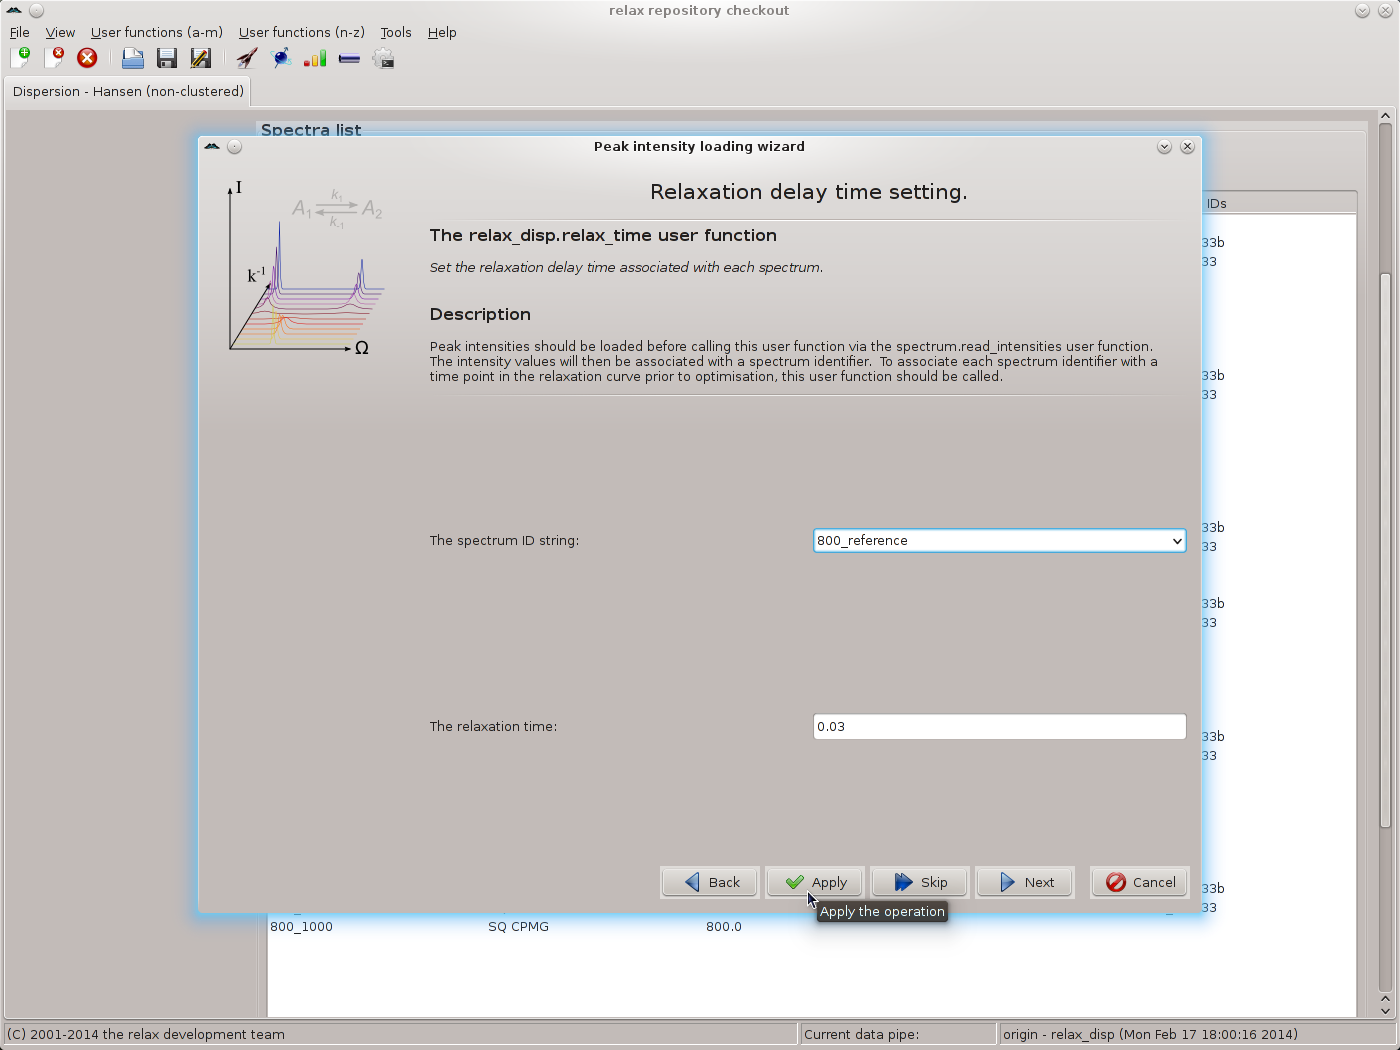
\includegraphics[
      width=0.9\textwidth,
      bb=14 14 1415 1065
    ]
    {graphics/screenshots/dispersion_analysis/spectrum_relax_time}
  }
\end{minipage}

Click on \guibutton{Next} to move to the \uf{relax\ufus{}disp\ufsep{}cpmg\ufus{}frq} user function wizard page.
If $\Ronerho$ data has been collected, the \uf{relax\ufus{}disp\ufsep{}spin\ufus{}lock\ufus{}field} user function wizard page would appear instead.
For the reference spectrum IDs, leave the CPMG frequency value blank and click on \guibutton{Apply}:

\begin{minipage}[h]{\linewidth}
  \centerline{
    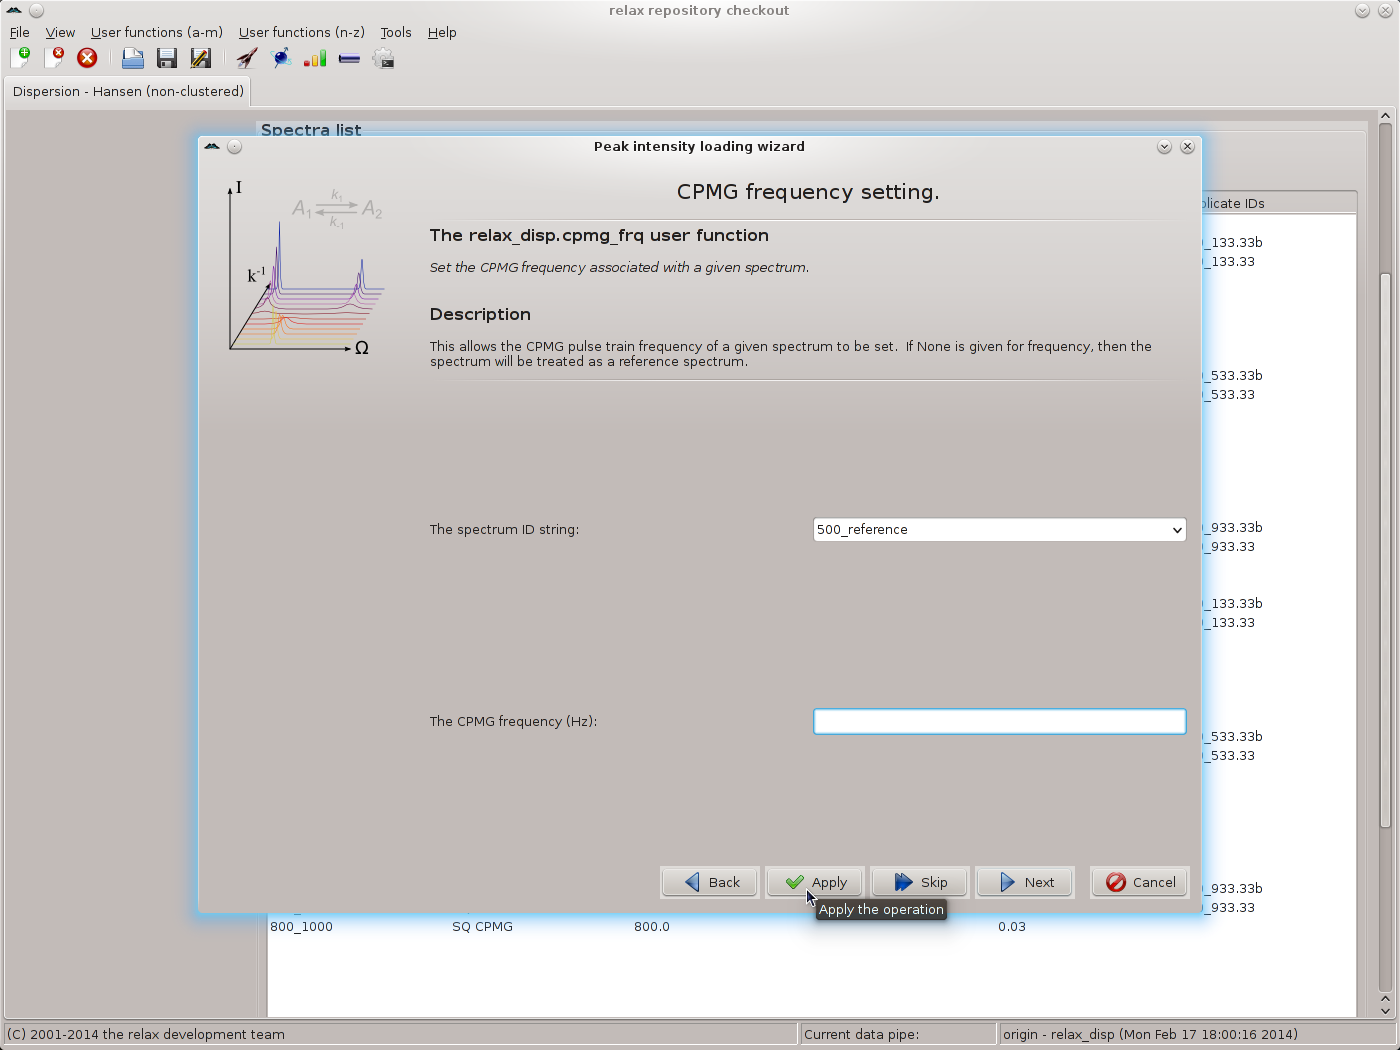
\includegraphics[
      width=0.9\textwidth,
      bb=14 14 1415 1065
    ]
    {graphics/screenshots/dispersion_analysis/spectrum_cpmg_frq}
  }
\end{minipage}

This will label these spectra as the reference.
For all other spectrum IDs, use the CPMG frequencies as given in the table above, using \guibutton{Apply} to execute the \uf{relax\ufus{}disp\ufsep{}cpmg\ufus{}frq} user function while staying on the same wizard page.
Click on \guibutton{Next} to finish.
You should now see the main relax window:

\begin{minipage}[h]{\linewidth}
  \centerline{
    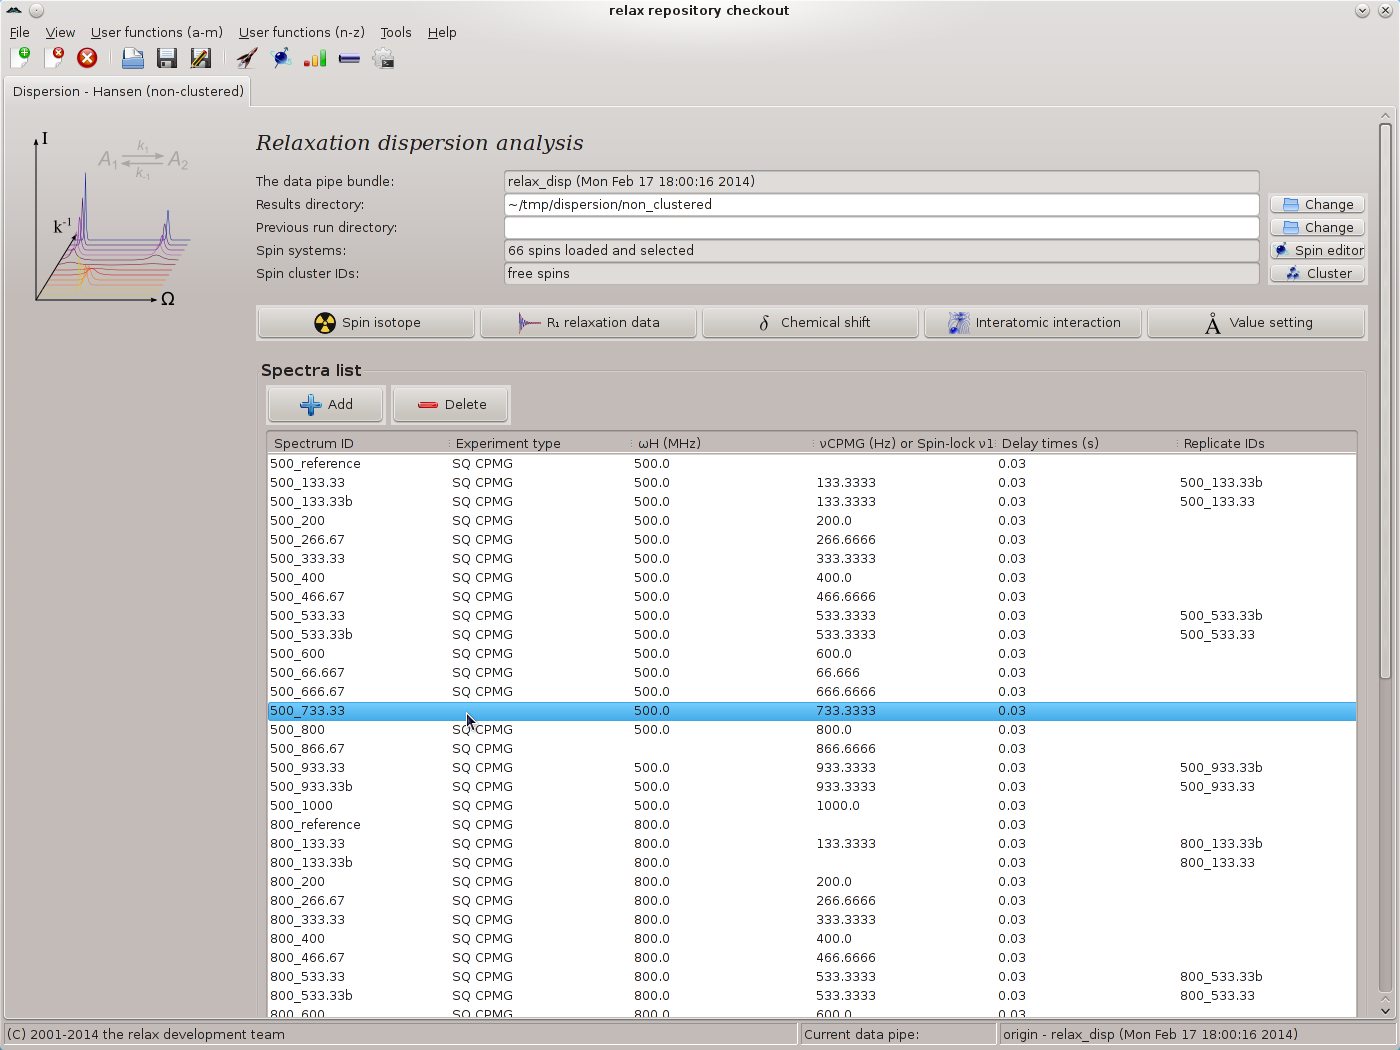
\includegraphics[
      width=0.9\textwidth,
      bb=14 14 1415 1065
    ]
    {graphics/screenshots/dispersion_analysis/data_loaded}
  }
\end{minipage}

In this screenshot it can be seen that some of the metadata is missing.
This often happens due to the large amounts of metadata specified in the peak intensity loading wizard and human error.
The missing metadata can now easily be filled in by right clicking on the corresponding row.
For example here the \guistring{500\_733.33} spectrum ID does not have the experiment type set.
Simply right click and select the \guimenuitemone{Set the experiment type} menu entry from the popup menu.
For the missing spectrometer frequency for the \guistring{500\_866.67} spectrum ID, the \guimenuitemone{Set the spectrometer frequency} menu entry can be used.
For the missing $\nucpmg$ value for the \guistring{800\_133.33} spectrum ID, the \guimenuitemone{Set the CPMG pulse frequency $\nucpmg$} menu entry can be used.
All of the metadata should be double and triple checked and fixed where required using the popup menu.
Any errors in this metadata would be catastrophic for the subsequent dispersion analysis.


% Choosing the models to optimise.
%~~~~~~~~~~~~~~~~~~~~~~~~~~~~~~~~~

\subsection{Dispersion GUI mode -- choosing the models to optimise}

The next step is to specify which relaxation dispersion models will be used in the analysis.
The number of models used should be limited based on your knowledge of the problem.
Depending on experimental information, a number of models can be ruled out.
For example for the data used in this tutorial, the exchange is known to be slow.
Hence all of the fast exchange models can be excluded.
For the conditions under which the various dispersion models can be used, please refer to the original references.
In relax many dispersion models are provided, however you should never use them all.

For this tutorial, we will only use the following dispersion models:
\begin{description}
  \item[`R2eff':]  This is essential for calculating the $\Rtwoeff$ values used as the input data for all other models (see section~\ref{sect: dispersion: R2eff model} on page~\pageref{sect: dispersion: R2eff model}).
  \item[`No Rex':]  This model will be important in the model selection stage to determine if any statistically significant relaxation dispersion is present in the $\Rtwoeff$ data (see section~\ref{sect: dispersion: No Rex model} on page~\pageref{sect: dispersion: No Rex model}).
  \item[`CR72':]  The Carver and Richards model for most time scales (see Section~\ref{sect: dispersion: CR72 model} on page~\pageref{sect: dispersion: CR72 model}).
    This is the standard model for slow timescale CPMG-type data (for fast timescales use the `LM63' model instead and for very slow exchange the `TSMFK01' model).
  \item[`NS CPMG 2-site expanded':]  The best and fastest of the numerical models for 2-site exchange (see Section~\ref{sect: dispersion: NS CPMG 2-site expanded model} on page~\pageref{sect: dispersion: NS CPMG 2-site expanded model}).
\end{description}

To chose which models will be used in the analysis, click on the \guibutton{Modify} button of the \guistring{Relaxation dispersion models} GUI element in the main relax window and change the model list to:

\begin{minipage}[h]{\linewidth}
  \centerline{
    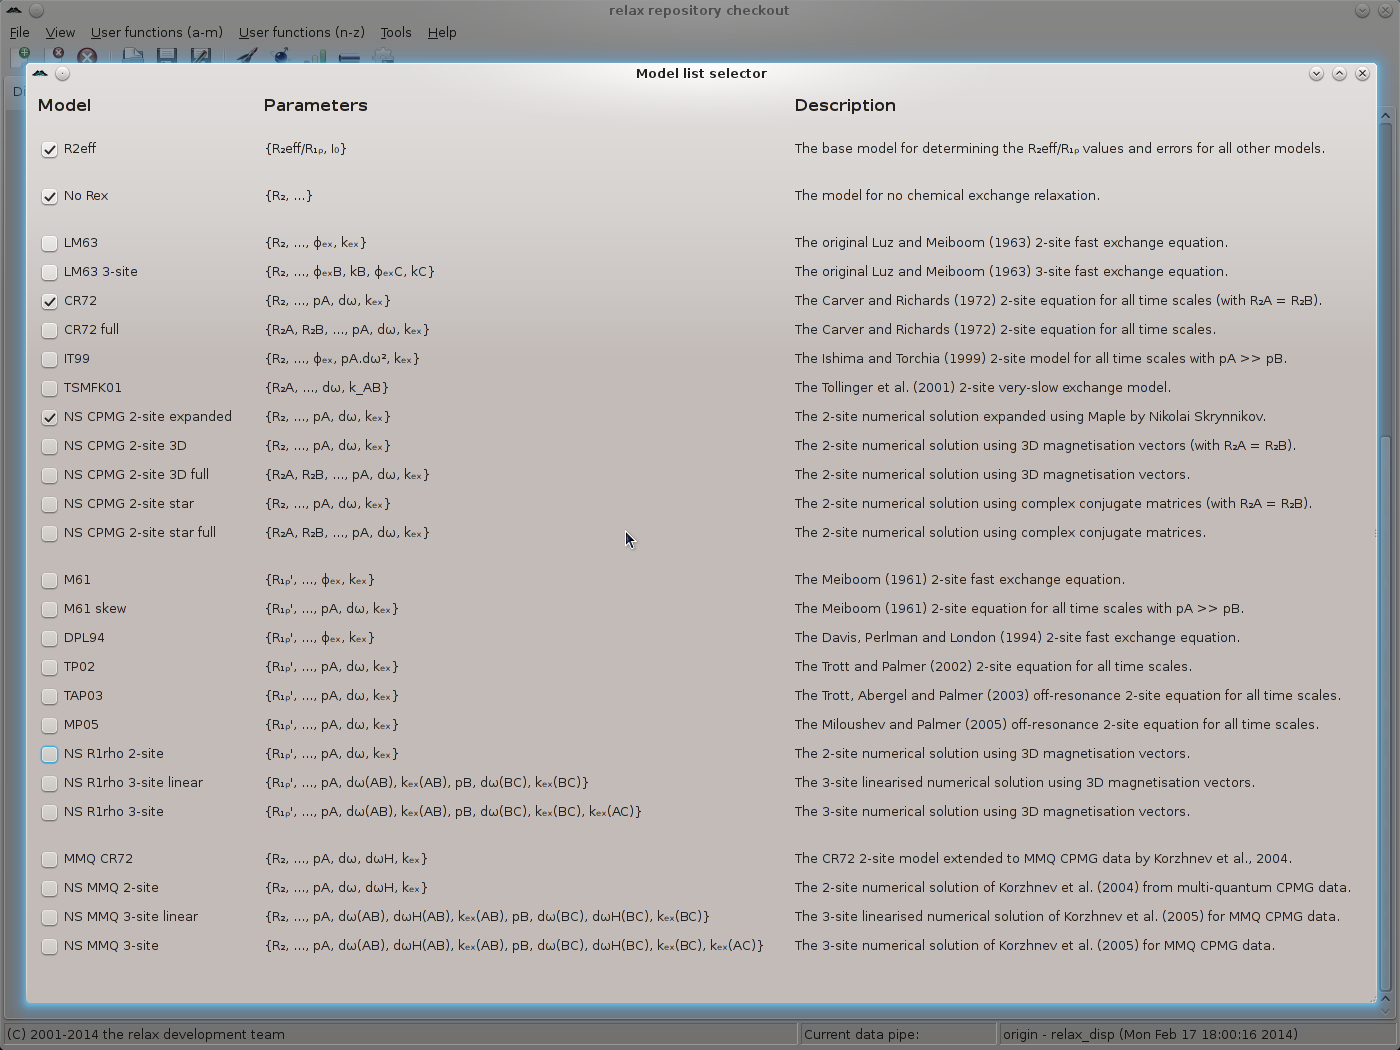
\includegraphics[
      width=0.9\textwidth,
      bb=14 14 1415 1065
    ]
    {graphics/screenshots/dispersion_analysis/model_selection}
  }
\end{minipage}

The \guistring{Pure numerical solution} flag will be left on \guistring{False}.
But if you prefer to only have results from the numerical models, this can be changed to \guistring{True} by clicking on the \guibutton{Toggle} button (note that the `CR72' model should nevertheless be used to speed up optimisation -- see section~\ref{sect: Dispersion parameter grid search} on page~\pageref{sect: Dispersion parameter grid search} for details).


% Optimisation settings.
%~~~~~~~~~~~~~~~~~~~~~~~

\subsection{Dispersion GUI mode -- optimisation settings}

The grid search increment number of 21 might be excessive, especially if the multiprocessor framework is not used to speed up calculations (see section~\ref{sect: Relaxation dispersion using OpenMPI} on page~\pageref{sect: Relaxation dispersion using OpenMPI}).
This value can be changed to 11, as this number is probably sufficient for most dispersion analyses.

Also for speed, the number of Monte Carlo simulations will be set to 200.
However for real analyses, the minimum number of 500 should be used for accurate parameter error estimates.
The \guistring{Per model error analysis} setting will be left to \guistring{False}.
And the \guistring{Insignificance level} will be left at 1.0 (see section~\ref{sect: Dispersion curve insignificance} on page~\pageref{sect: Dispersion curve insignificance}).


% Execution of the non-clustered analysis.
%~~~~~~~~~~~~~~~~~~~~~~~~~~~~~~~~~~~~~~~~~

\subsection{Dispersion GUI mode -- execution of the non-clustered analysis}

To start the analysis, simply click the \guibutton{Execute} button to start the analysis:

\begin{minipage}[h]{\linewidth}
  \centerline{
    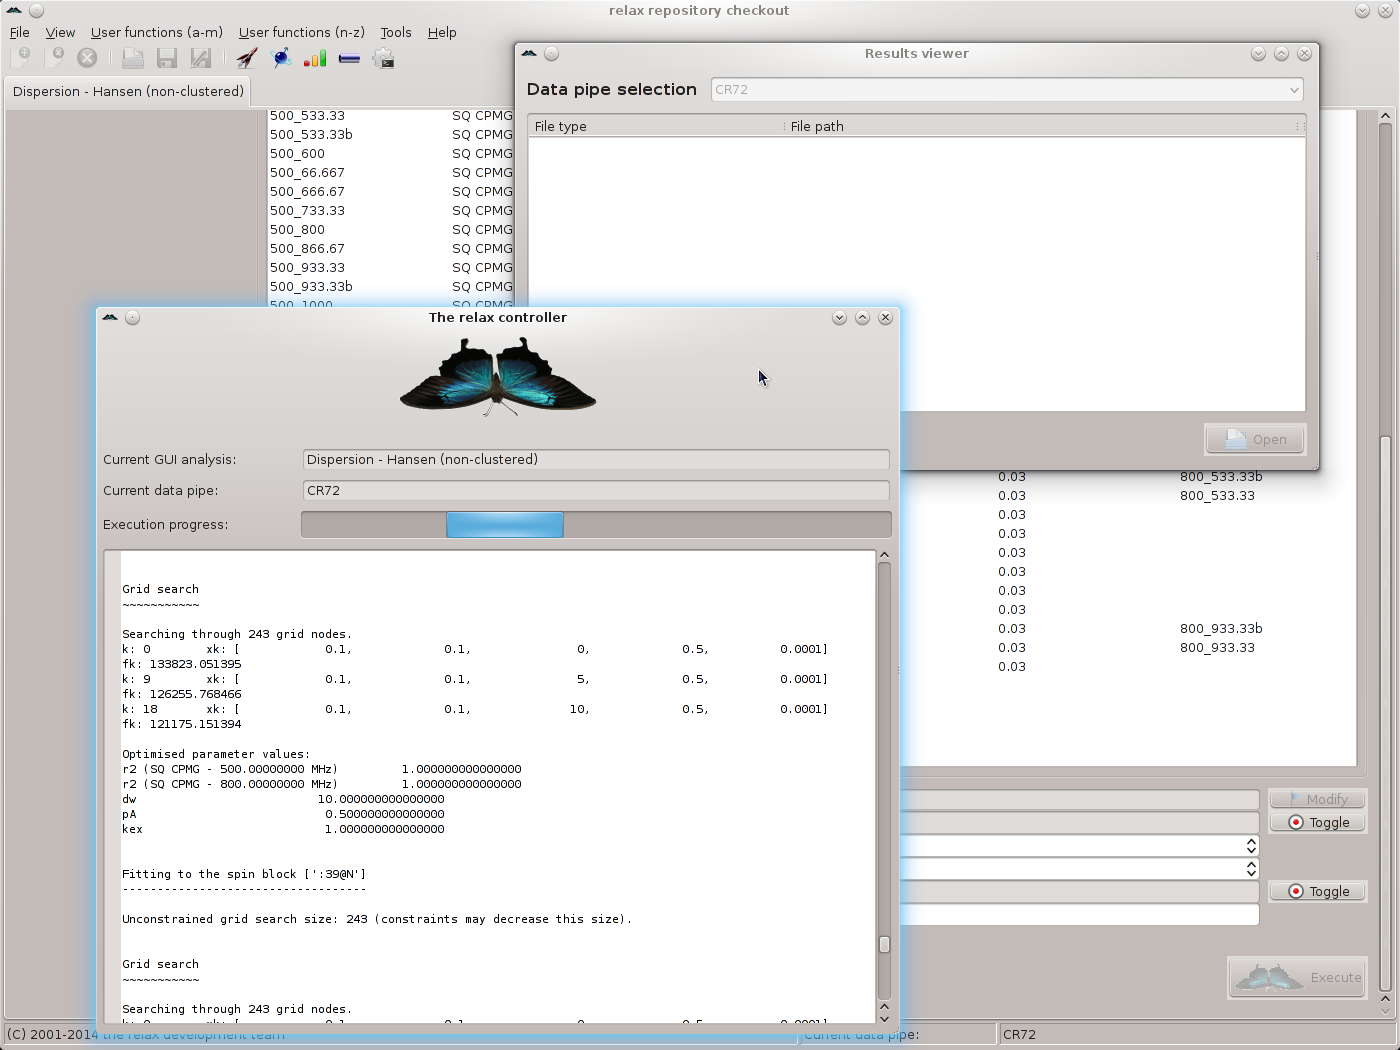
\includegraphics[
      width=0.9\textwidth,
      bb=14 14 1415 1065
    ]
    {graphics/screenshots/dispersion_analysis/executing}
  }
\end{minipage}

If the setup is incomplete, an error window will appear describing the problem.
If a slow computer is used without Gary Thompson's multiprocessor, the calculation time could take one to several days.
But on a modern, multi-core system using the OpenMPI multiprocessor, the calculation should only take hours.
Once complete, you will see:

\begin{minipage}[h]{\linewidth}
  \centerline{
    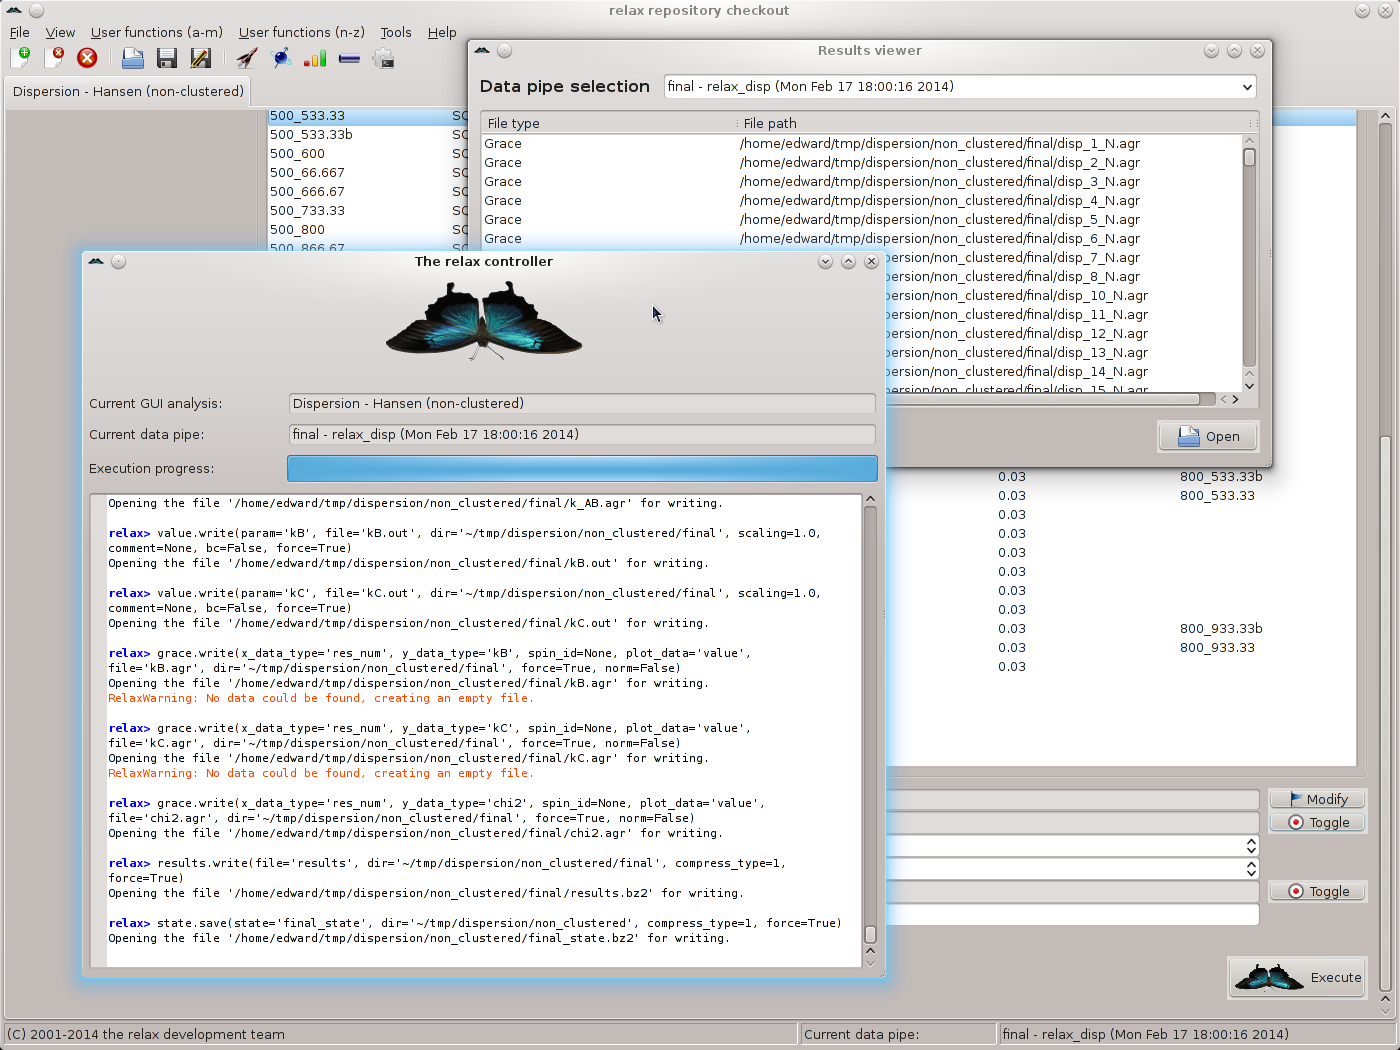
\includegraphics[
      width=0.9\textwidth,
      bb=14 14 1415 1065
    ]
    {graphics/screenshots/dispersion_analysis/fin_non_clustered}
  }
\end{minipage}

The relax controller window can be closed.
At all stages of the analysis, the logs should be checked for all warnings.
For example searching for the text `RelaxWarning' in the log file \directory{$\sim$\ossep{}dispersion\ossep{}log\osus{}non\osus{}clustered}, the only warnings can be seen at the end of the analysis.
These can be seen to be harmless as they are indicating that certain Grace 2D plots contain no data -- specifically those for dispersion parameters not present in the set of models optimised.
Any other warnings should however be very carefully noted and checked as these could be pointing to a serious problem.


% Inspection of the results.
%~~~~~~~~~~~~~~~~~~~~~~~~~~~

\subsection{Dispersion GUI mode -- inspection of the results}

To view the results of the analysis, the relax results window will have been automatically opened.
If it was closed, click on the \guimenuitemtwo{View}{Results viewer} menu entry or the \guibutton{Results viewer window} button in the toolbar to open the window.
This window will list all of the \file{*.out} text files and \file{*.agr} 2D Grace plots created by the auto-analysis.
By double clicking on the file, these can be opened.
The operating specific text editor will be launched for the text files.
For the Grace files, the installed Grace version (Xmgrace, QtGrace, or GraceGTK) will be launched.

Firstly, to see which models have been chosen for the spin systems and which have no statistically significant dispersion, find the \file{model.out} file and double click on it.
You should see the following:

\begin{lstlisting}[basicstyle=\ttfamily \scriptsize,numbers=none]
# Parameter description:  The dispersion model.
#
# mol_name    res_num    res_name    spin_num    spin_name    value                        error    
None          1          GLY         None        N            'NS CPMG 2-site expanded'    None     
None          2          GLY         None        N            'No Rex'                     None     
None          3          GLY         None        N            'No Rex'                     None     
None          4          GLY         None        N            'No Rex'                     None     
None          5          GLY         None        N            'CR72'                       None     
None          6          GLY         None        N            'No Rex'                     None     
None          7          GLY         None        N            'No Rex'                     None     
None          8          GLY         None        N            'NS CPMG 2-site expanded'    None     
None          9          GLY         None        N            None                         None     
None          10         GLY         None        N            'No Rex'                     None     
None          11         GLY         None        N            'No Rex'                     None     
None          12         GLY         None        N            'NS CPMG 2-site expanded'    None     
None          13         GLY         None        N            'No Rex'                     None     
None          14         GLY         None        N            'CR72'                       None     
None          15         GLY         None        N            'No Rex'                     None     
None          16         GLY         None        N            'No Rex'                     None     
None          17         GLY         None        N            'No Rex'                     None     
None          18         GLY         None        N            'No Rex'                     None     
None          19         GLY         None        N            'No Rex'                     None     
None          20         GLY         None        N            'No Rex'                     None     
None          21         GLY         None        N            'CR72'                       None     
None          22         GLY         None        N            'No Rex'                     None     
None          23         GLY         None        N            'CR72'                       None     
None          24         GLY         None        N            'No Rex'                     None     
None          25         GLY         None        N            'No Rex'                     None     
None          26         GLY         None        N            'CR72'                       None     
None          27         GLY         None        N            None                         None     
None          28         GLY         None        N            None                         None     
None          29         GLY         None        N            'No Rex'                     None     
None          30         GLY         None        N            None                         None     
None          31         GLY         None        N            'NS CPMG 2-site expanded'    None     
None          32         GLY         None        N            'NS CPMG 2-site expanded'    None     
None          33         GLY         None        N            'No Rex'                     None     
None          34         GLY         None        N            'NS CPMG 2-site expanded'    None     
None          35         GLY         None        N            'No Rex'                     None     
None          36         GLY         None        N            'No Rex'                     None     
None          37         GLY         None        N            'No Rex'                     None     
None          38         GLY         None        N            'NS CPMG 2-site expanded'    None     
None          39         GLY         None        N            'NS CPMG 2-site expanded'    None     
None          40         GLY         None        N            'No Rex'                     None     
None          41         GLY         None        N            'No Rex'                     None     
None          42         GLY         None        N            'NS CPMG 2-site expanded'    None     
None          43         GLY         None        N            'No Rex'                     None     
None          44         GLY         None        N            'No Rex'                     None     
None          45         GLY         None        N            'NS CPMG 2-site expanded'    None     
None          46         GLY         None        N            'NS CPMG 2-site expanded'    None     
None          47         GLY         None        N            'NS CPMG 2-site expanded'    None     
None          48         GLY         None        N            'No Rex'                     None     
None          49         GLY         None        N            'No Rex'                     None     
None          50         GLY         None        N            'No Rex'                     None     
None          51         GLY         None        N            'CR72'                       None     
None          52         GLY         None        N            'NS CPMG 2-site expanded'    None     
None          53         GLY         None        N            'NS CPMG 2-site expanded'    None     
None          54         GLY         None        N            None                         None     
None          55         GLY         None        N            'NS CPMG 2-site expanded'    None     
None          56         GLY         None        N            'No Rex'                     None     
None          57         GLY         None        N            'No Rex'                     None     
None          58         GLY         None        N            'No Rex'                     None     
None          59         GLY         None        N            'CR72'                       None     
None          60         GLY         None        N            'No Rex'                     None     
None          61         GLY         None        N            'NS CPMG 2-site expanded'    None     
None          62         GLY         None        N            'NS CPMG 2-site expanded'    None     
None          63         GLY         None        N            'CR72'                       None     
None          64         GLY         None        N            'CR72'                       None     
None          65         GLY         None        N            'CR72'                       None     
None          66         GLY         None        N            'NS CPMG 2-site expanded'    None     
None          67         GLY         None        N            'NS CPMG 2-site expanded'    None     
None          68         GLY         None        N            None                         None     
None          69         GLY         None        N            None                         None     
None          70         GLY         None        N            'NS CPMG 2-site expanded'    None     
None          71         GLY         None        N            'NS CPMG 2-site expanded'    None     
None          72         GLY         None        N            'NS CPMG 2-site expanded'    None     
None          73         GLY         None        N            'CR72'                       None     
\end{lstlisting}

Excluding the deselected spin systems with the model `None' and those with no statistically significant dispersion, `No Rex', it can be seen that in some cased the `CR72' model is selected whereas in others the `NS CPMG 2-site expanded' model is selected.
The differences between the `CR72' analytic model and the `NS CPMG 2-site expanded' numeric model are insignificant.
To see this, open the \file{CR72\ossep{}chi2.out} and \file{NS CPMG 2-site expanded\ossep{}chi2.out} text files in the \directory{$\sim$\ossep{}dispersion\ossep{}log\osus{}non\osus{}clustered} directory and compare the optimised chi-squared values (this can be performed with the mouse by using the pipe editor window, changing the current data pipe, and double clicking on the files in the results viewer window for each data pipe -- see below for more details).

To see which spins have been assigned the model `No Rex' due to the $\Rtwoeff/\Ronerho$ insignificance level of 1.0 rad/s, search the log messages for `insignificance'.
You should see:

\begin{lstlisting}[basicstyle=\ttfamily \tiny,language=relax_log,numbers=none]
relax> relax_disp.insignificance(level=1.0)
Deselecting spin ':2@N', the maximum dispersion curve difference for all curves is 0.772528040762 rad/s.
Deselecting spin ':3@N', the maximum dispersion curve difference for all curves is 0.572686080104 rad/s.
Deselecting spin ':4@N', the maximum dispersion curve difference for all curves is 0.20753288407 rad/s.
Deselecting spin ':7@N', the maximum dispersion curve difference for all curves is 0.184120905625 rad/s.
Deselecting spin ':10@N', the maximum dispersion curve difference for all curves is 0.746360942576 rad/s.
Deselecting spin ':11@N', the maximum dispersion curve difference for all curves is 0.372702361421 rad/s.
Deselecting spin ':13@N', the maximum dispersion curve difference for all curves is 0.261522940719 rad/s.
Deselecting spin ':15@N', the maximum dispersion curve difference for all curves is 0.743965404051 rad/s.
Deselecting spin ':16@N', the maximum dispersion curve difference for all curves is 0.198783344901 rad/s.
Deselecting spin ':17@N', the maximum dispersion curve difference for all curves is 0.469568638477 rad/s.
Deselecting spin ':18@N', the maximum dispersion curve difference for all curves is 0.720840385548 rad/s.
Deselecting spin ':19@N', the maximum dispersion curve difference for all curves is 0.290773963568 rad/s.
Deselecting spin ':20@N', the maximum dispersion curve difference for all curves is 0.983669594767 rad/s.
Deselecting spin ':22@N', the maximum dispersion curve difference for all curves is 0.507488886605 rad/s.
Deselecting spin ':24@N', the maximum dispersion curve difference for all curves is 0.984086643389 rad/s.
Deselecting spin ':25@N', the maximum dispersion curve difference for all curves is 0.638104572082 rad/s.
Deselecting spin ':29@N', the maximum dispersion curve difference for all curves is 0.525261970487 rad/s.
Deselecting spin ':33@N', the maximum dispersion curve difference for all curves is 0.822112754666 rad/s.
Deselecting spin ':35@N', the maximum dispersion curve difference for all curves is 0.713976877685 rad/s.
Deselecting spin ':36@N', the maximum dispersion curve difference for all curves is 0.413602640091 rad/s.
Deselecting spin ':37@N', the maximum dispersion curve difference for all curves is 0.302953864843 rad/s.
Deselecting spin ':40@N', the maximum dispersion curve difference for all curves is 0.401535026435 rad/s.
Deselecting spin ':41@N', the maximum dispersion curve difference for all curves is 0.805657060225 rad/s.
Deselecting spin ':43@N', the maximum dispersion curve difference for all curves is 0.582523964429 rad/s.
Deselecting spin ':44@N', the maximum dispersion curve difference for all curves is 0.325638582443 rad/s.
Deselecting spin ':45@N', the maximum dispersion curve difference for all curves is 0.947956877688 rad/s.
Deselecting spin ':49@N', the maximum dispersion curve difference for all curves is 0.872396631779 rad/s.
Deselecting spin ':50@N', the maximum dispersion curve difference for all curves is 0.403543891199 rad/s.
Deselecting spin ':56@N', the maximum dispersion curve difference for all curves is 0.468272490195 rad/s.
Deselecting spin ':57@N', the maximum dispersion curve difference for all curves is 0.634215047495 rad/s.
Deselecting spin ':58@N', the maximum dispersion curve difference for all curves is 0.953109267554 rad/s.
\end{lstlisting}

Search for `eliminate' to see which models have been removed due to the model elimination step (see section~\ref{sect: relaxation dispersion model elimination} on page~\pageref{sect: relaxation dispersion model elimination} for details).
For example for the CR72 model:

\begin{lstlisting}[basicstyle=\ttfamily \tiny,language=relax_log,numbers=none]
relax> eliminate(function=None, args=None)
Data pipe 'CR72 - relax_disp (Mon Feb 17 18:00:16 2014)':  The pA parameter of 0.50003 is less than  0.50100, eliminating the spin cluster [':6@N'].
Data pipe 'CR72 - relax_disp (Mon Feb 17 18:00:16 2014)':  The pA parameter of 0.50001 is less than  0.50100, eliminating the spin cluster [':38@N'].
Data pipe 'CR72 - relax_disp (Mon Feb 17 18:00:16 2014)':  The pA parameter of 0.50001 is less than  0.50100, eliminating the spin cluster [':42@N'].
Data pipe 'CR72 - relax_disp (Mon Feb 17 18:00:16 2014)':  The pA parameter of 0.50001 is less than  0.50100, eliminating the spin cluster [':45@N'].
Data pipe 'CR72 - relax_disp (Mon Feb 17 18:00:16 2014)':  The pA parameter of 0.50000 is less than  0.50100, eliminating the spin cluster [':46@N'].
Data pipe 'CR72 - relax_disp (Mon Feb 17 18:00:16 2014)':  The pA parameter of 0.50002 is less than  0.50100, eliminating the spin cluster [':47@N'].
Data pipe 'CR72 - relax_disp (Mon Feb 17 18:00:16 2014)':  The pA parameter of 0.50000 is less than  0.50100, eliminating the spin cluster [':48@N'].
Data pipe 'CR72 - relax_disp (Mon Feb 17 18:00:16 2014)':  The pA parameter of 0.50002 is less than  0.50100, eliminating the spin cluster [':60@N'].
Data pipe 'CR72 - relax_disp (Mon Feb 17 18:00:16 2014)':  The pA parameter of 0.50000 is less than  0.50100, eliminating the spin cluster [':62@N'].
\end{lstlisting}

To see the optimised parameter values, double click on the \file{kex.agr} file to see the exchange rates.
This will open the \uf{grace\ufsep{}view} user function window by which the file can be opened.
The default settings produces the following graph:

\begin{minipage}[h]{\linewidth}
  \centerline{
    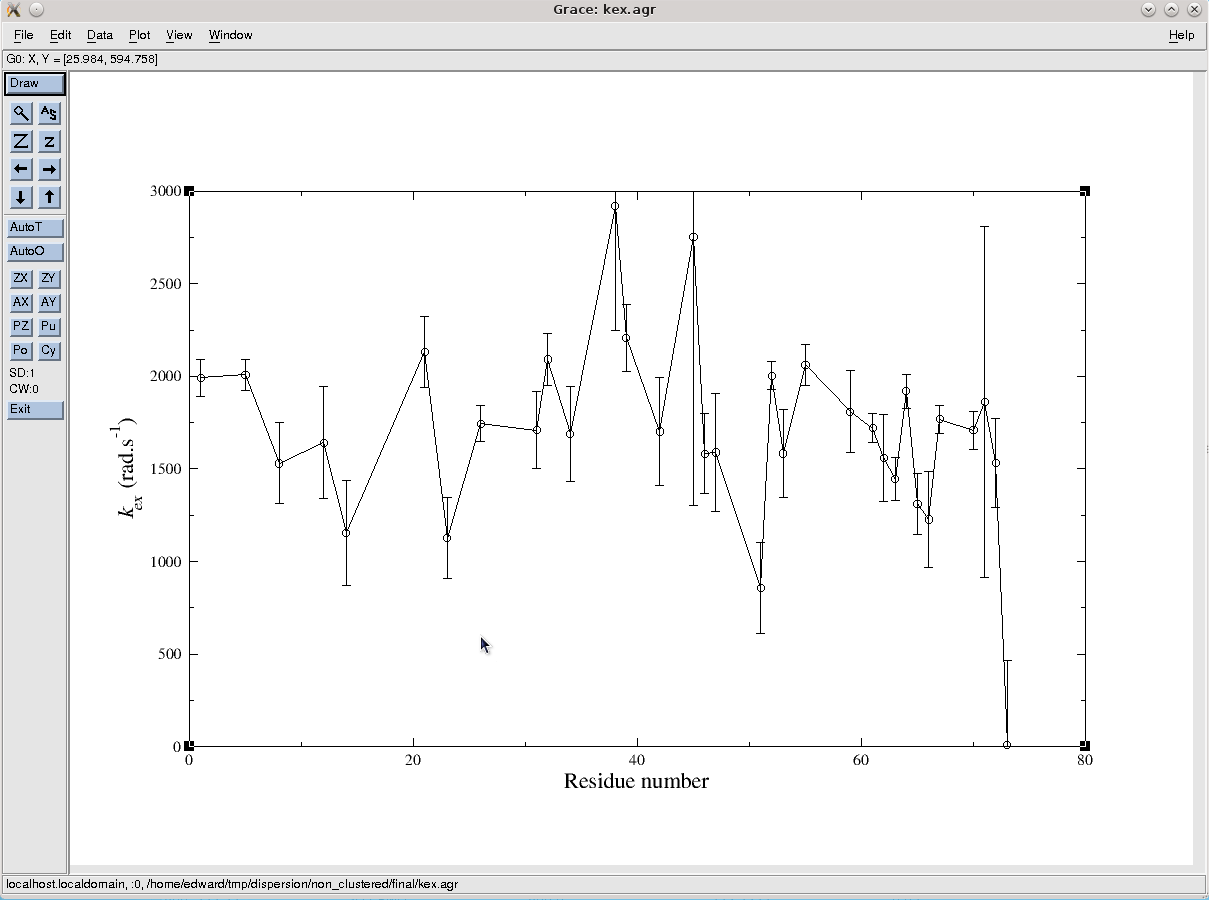
\includegraphics[
      width=0.9\textwidth,
      bb=14 14 1231 922
    ]
    {graphics/screenshots/dispersion_analysis/grace_kex}
  }
\end{minipage}

The exchange rate for most spins experiencing exchange is between 1000 and 2000~s$^{-1}$.
Opening the \file{pA.agr} file, it can be seen that the population of state A is approximately 0.98.
A number of spins have much lower values than this, but their errors are huge meaning that all but 3 are statistically the same as 0.98 (note that a proper ANOVA statistics analysis would be required to make such statements).

To see one of the dispersion curves, open the \file{disp\osus{}64\osus{}N.agr} file in Grace.
The default settings will produce the graph:

\begin{minipage}[h]{\linewidth}
  \centerline{
    \includegraphics[
      width=\textwidth,
      bb=14 14 788 523
    ]
    {graphics/screenshots/dispersion_analysis/disp_64_N}
  }
\end{minipage}

To improve the appearance of this plot, please refer to the Grace software documentation.


% Comparing models.
%~~~~~~~~~~~~~~~~~~

\subsection{Dispersion GUI mode -- comparing models}

To compare the results of the different optimised models, the pipe editor window can be used to switch between the data pipes containing the results of the individual models.
Select the \guimenuitemtwo{View}{Data pipe editor} menu entry.
Right click on the model of interest and select \guimenuitemone{Switch to this pipe}:

\begin{minipage}[h]{\linewidth}
  \centerline{
    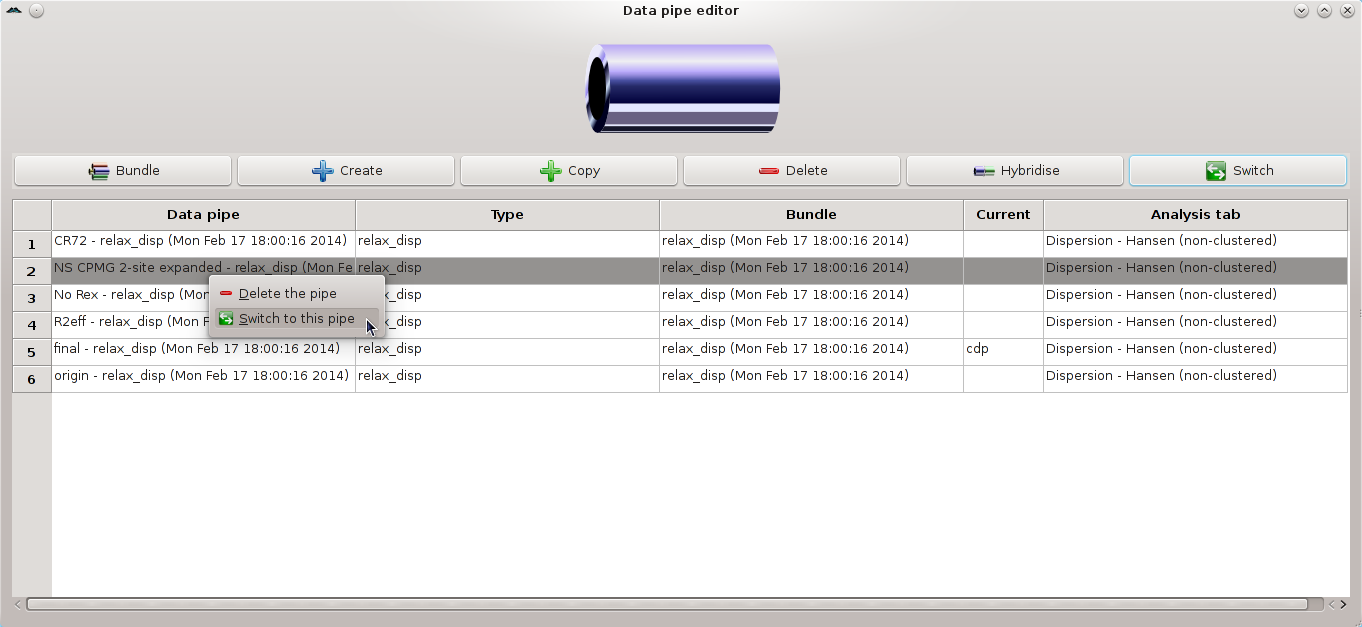
\includegraphics[
      width=0.9\textwidth,
      bb=14 14 1377 642
    ]
    {graphics/screenshots/dispersion_analysis/pipe_window}
  }
\end{minipage}

The results viewer window can then be used to open the text files and Grace plots for that model.
Switch to the data pipe of another model and open the same file to compare the results.


% The clustered analysis.
%~~~~~~~~~~~~~~~~~~~~~~~~

\subsection{Dispersion GUI mode -- the clustered analysis}

Before the second analysis with spin clustering will be performed, the relax state will be saved in the file \file{state.bz2} and the program closed.
To store the details of the second analysis in a separate log file, relax will be restarted with the command:

\example{\$ mpirun -np 8 /data/relax/relax-trunk/relax --multi='mpi4py' --log $\sim$/tmp/dispersion/log\_clustered --gui}

When the GUI has started, load the \file{state.bz2} file.
If relax is not restarted, all messages will be in a single log file.

For the clustered analysis, we will focus on one group of spins -- those from residues :59 to :67.
These can be seen to have very similar dynamics:

\begin{lstlisting}[basicstyle=\ttfamily \scriptsize,numbers=none]
# Parameter description:  The population for state A.
#
# mol_name  res_num  res_name  spin_num  spin_name  value                 error                   
[snip]
None        59       GLY       None      N             0.991169677577733    0.0254974551085798    
None        60       GLY       None      N          None                  None                    
None        61       GLY       None      N             0.989169345780449  0.000173707304433962    
None        62       GLY       None      N             0.892612114003636     0.156741312688688    
None        63       GLY       None      N             0.991579380015928   0.00101555844987099    
None        64       GLY       None      N             0.983519617639107   0.00141882200997569    
None        65       GLY       None      N             0.993831316342131   0.00840481515172743    
None        66       GLY       None      N             0.996816227018878   0.00495523034494496    
None        67       GLY       None      N             0.987206586948786  0.000217099775069814    
[snip]
\end{lstlisting}

\begin{lstlisting}[basicstyle=\ttfamily \scriptsize,numbers=none]
# Parameter description:  The exchange rate.
#
# mol_name  res_num  res_name  spin_num  spin_name  value                 error                   
[snip]
None        59       GLY       None      N              1856.39029180567      258.796681611922    
None        60       GLY       None      N          None                  None                    
None        61       GLY       None      N              1706.42820099893      79.5779060629935    
None        62       GLY       None      N              1560.77926730839      246.876174669559    
None        63       GLY       None      N              1448.69535431372      121.940593279104    
None        64       GLY       None      N               1922.2405164604      96.0557804598977    
None        65       GLY       None      N               1333.8423680145      168.000554346898    
None        66       GLY       None      N              1243.45993122534      238.215664971556    
None        67       GLY       None      N              1753.32557147779      78.2028166128168    
[snip]
\end{lstlisting}

All other spins will be deselected.

From the non-clustered results, it could be argued that all spins in the entire system experience the same dynamic process, i.e.\ they have the same $\pA$ and $\kex$ values.
Such an analysis could be performed at a later stage if desired.
The dispersion curves for the residue :60 could also be inspected to see that dispersion is likely to be present and another clustered analysis including this spin performed.
The number of clustered analyses performed is up to the user -- imagination is the only limit.

To start the analysis, open the analysis selection wizard as was performed previously.
Name the analysis as `Dispersion - Hansen (clustered :59 to :67)'.
Once the analysis is initialised, change the results directory to \directory{$\sim$\ossep{}tmp\ossep{}dispersion\ossep{}clustered}.
To use the results of the previous analysis to speed up this analysis, as clustering will cause the grid search to be impossibly long, change the \guistring{Previous run directory} value to \directory{$\sim$\ossep{}tmp\ossep{}dispersion\ossep{}non\osus{}clustered}.

Set up the spin systems as for the non-clustered analysis.
This time however deselect all spins except for those of residues :59 to :67 (excluding :60).
This can be performed by right clicking on the spins in the spin viewer window.

The next step is to cluster these eight spins.
In the \guistring{Spin cluster IDs} GUI element, click on the \guibutton{Cluster} button.
This launches the \uf{relax\ufus{}disp\ufsep{}cluster} user function.
Set the cluster ID to \guistring{res\_59\_to\_67}, for example, and the spin ID string to \guistring{:59-67} (this says all residues from :59 to :67, see section~\ref{sect: spin ID} on page~\pageref{sect: spin ID} for details):

\begin{minipage}[h]{\linewidth}
  \centerline{
    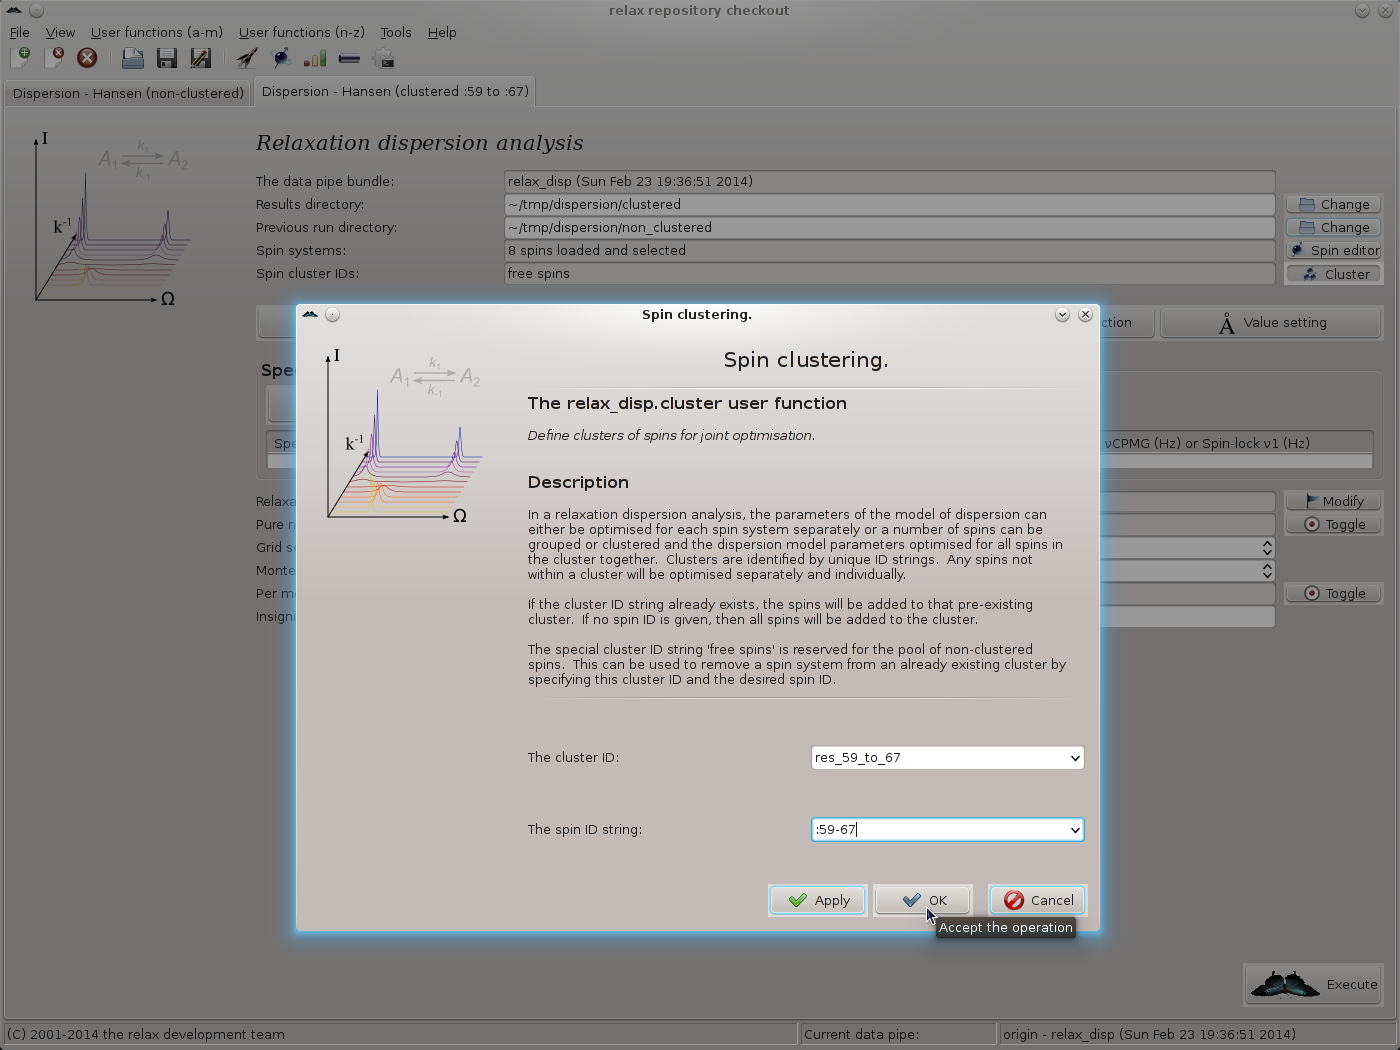
\includegraphics[
      width=0.9\textwidth,
      bb=14 14 1415 1065
    ]
    {graphics/screenshots/dispersion_analysis/relax_disp_cluster}
  }
\end{minipage}

As spin :60 is deselected, that residue will be skipped in the analysis.

Then set the spin isotope and load all of the Sparky peak lists as before.
Chose the models `R2eff', `No Rex', `CR72', and `NS CPMG 2-site expanded'.
As the `CR72' and `NS CPMG 2-site expanded' were seen as being statistically equivalent in the non-clustered analysis, click on the \guibutton{Toggle} button of the \guistring{Pure numerical solutions} GUI element to avoid the `CR72' model in the model selection step.
Actually, as the initial parameters for the `NS CPMG 2-site expanded' model in the dispersion auto-analysis will be taken as the average from the non-clustered analysis, the `CR72' model could be completely skipped.

Ignore the grid search increment setting as this will have no effect.
No grid searches will be performed because the results from the non-clustered analysis will be used as the optimisation starting point.
Set the Monte Carlo simulations to 200.
The main window should now look like:

\begin{minipage}[h]{\linewidth}
  \centerline{
    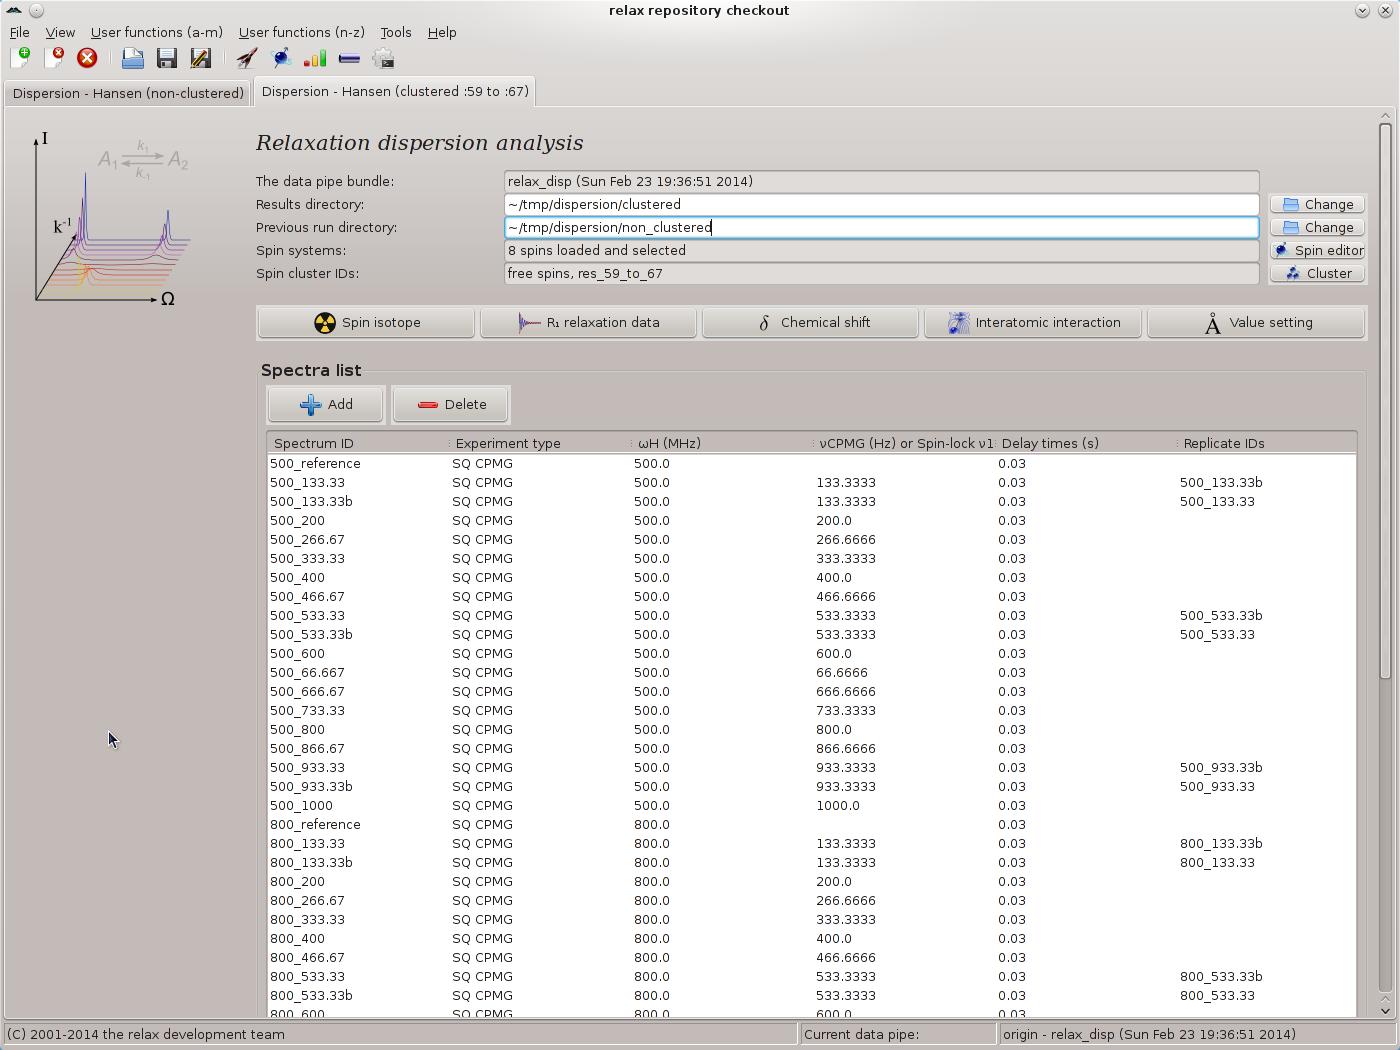
\includegraphics[
      width=0.9\textwidth,
      bb=14 14 1415 1065
    ]
    {graphics/screenshots/dispersion_analysis/clustered_setup}
  }
\end{minipage}

Start the analysis by clicking on the \guibutton{Execute} button.
You should notice that the spin cluster printout in the log messages in the relax controller window now show the text:

\begin{lstlisting}[numbers=none]
The spin cluster [':59', ':60', ':61', ':62', ':63', ':64', ':65', ':66', ':67'].
\end{lstlisting}

As residue 60 is deselected, it will not be used in the optimisation or any part of the analysis.
The full analysis should take a few hours to complete.


% Comparison of the analyses.
%~~~~~~~~~~~~~~~~~~~~~~~~~~~~

\subsection{Dispersion GUI mode -- comparison of the analyses}

To statistically compare the non-clustered and clustered analyses, the advanced Akaike's Information Criterion (AIC) as derived in \cite{dAuvergneGooley03} can be used.
This information is stored within the recorded log files.
Open the \file{$\sim$/tmp/dispersion/log\_non\_clustered} file and search for the model selection section.
The text for residues 59 to 67 should be:

\begin{lstlisting}[basicstyle=\ttfamily \tiny,language=relax_log,numbers=none]
The spin cluster [':59@N'].
# Data pipe                                                        Num_params_(k)    Num_data_sets_(n)    Chi2          Criterion     
No Rex - relax_disp (Mon Feb 17 18:00:16 2014)                     2                 30                   1577.42286    1581.42286    
CR72 - relax_disp (Mon Feb 17 18:00:16 2014)                       5                 30                   31.48415      41.48415      
NS CPMG 2-site expanded - relax_disp (Mon Feb 17 18:00:16 2014)    5                 30                   31.84758      41.84758      
The model from the data pipe 'CR72 - relax_disp (Mon Feb 17 18:00:16 2014)' has been selected.


The spin cluster [':60@N'].
# Data pipe                                       Num_params_(k)    Num_data_sets_(n)    Chi2          Criterion     
No Rex - relax_disp (Mon Feb 17 18:00:16 2014)    2                 30                   2647.97449    2651.97449    
The model from the data pipe 'No Rex - relax_disp (Mon Feb 17 18:00:16 2014)' has been selected.


The spin cluster [':61@N'].
# Data pipe                                                        Num_params_(k)    Num_data_sets_(n)    Chi2           Criterion      
No Rex - relax_disp (Mon Feb 17 18:00:16 2014)                     2                 30                   15019.24382    15023.24382    
CR72 - relax_disp (Mon Feb 17 18:00:16 2014)                       5                 30                   77.50622       87.50622       
NS CPMG 2-site expanded - relax_disp (Mon Feb 17 18:00:16 2014)    5                 30                   74.73334       84.73334       
The model from the data pipe 'NS CPMG 2-site expanded - relax_disp (Mon Feb 17 18:00:16 2014)' has been selected.


The spin cluster [':62@N'].
# Data pipe                                                        Num_params_(k)    Num_data_sets_(n)    Chi2         Criterion    
No Rex - relax_disp (Mon Feb 17 18:00:16 2014)                     2                 30                   722.91592    726.91592    
NS CPMG 2-site expanded - relax_disp (Mon Feb 17 18:00:16 2014)    5                 30                   30.11618     40.11618     
The model from the data pipe 'NS CPMG 2-site expanded - relax_disp (Mon Feb 17 18:00:16 2014)' has been selected.


The spin cluster [':63@N'].
# Data pipe                                                        Num_params_(k)    Num_data_sets_(n)    Chi2          Criterion     
No Rex - relax_disp (Mon Feb 17 18:00:16 2014)                     2                 30                   5455.72135    5459.72135    
CR72 - relax_disp (Mon Feb 17 18:00:16 2014)                       5                 30                   58.56731      68.56731      
NS CPMG 2-site expanded - relax_disp (Mon Feb 17 18:00:16 2014)    5                 30                   59.90738      69.90738      
The model from the data pipe 'CR72 - relax_disp (Mon Feb 17 18:00:16 2014)' has been selected.


The spin cluster [':64@N'].
# Data pipe                                                        Num_params_(k)    Num_data_sets_(n)    Chi2           Criterion      
No Rex - relax_disp (Mon Feb 17 18:00:16 2014)                     2                 30                   13736.91051    13740.91051    
CR72 - relax_disp (Mon Feb 17 18:00:16 2014)                       5                 30                   28.66223       38.66223       
NS CPMG 2-site expanded - relax_disp (Mon Feb 17 18:00:16 2014)    5                 30                   29.54008       39.54008       
The model from the data pipe 'CR72 - relax_disp (Mon Feb 17 18:00:16 2014)' has been selected.


The spin cluster [':65@N'].
# Data pipe                                                        Num_params_(k)    Num_data_sets_(n)    Chi2          Criterion     
No Rex - relax_disp (Mon Feb 17 18:00:16 2014)                     2                 30                   2498.29408    2502.29408    
CR72 - relax_disp (Mon Feb 17 18:00:16 2014)                       5                 30                   35.13518      45.13518      
NS CPMG 2-site expanded - relax_disp (Mon Feb 17 18:00:16 2014)    5                 30                   36.17043      46.17043      
The model from the data pipe 'CR72 - relax_disp (Mon Feb 17 18:00:16 2014)' has been selected.


The spin cluster [':66@N'].
# Data pipe                                                        Num_params_(k)    Num_data_sets_(n)    Chi2         Criterion    
No Rex - relax_disp (Mon Feb 17 18:00:16 2014)                     2                 30                   962.74016    966.74016    
CR72 - relax_disp (Mon Feb 17 18:00:16 2014)                       5                 30                   15.02929     25.02929     
NS CPMG 2-site expanded - relax_disp (Mon Feb 17 18:00:16 2014)    5                 30                   15.08439     25.08439     
The model from the data pipe 'CR72 - relax_disp (Mon Feb 17 18:00:16 2014)' has been selected.


The spin cluster [':67@N'].
# Data pipe                                                        Num_params_(k)    Num_data_sets_(n)    Chi2           Criterion      
No Rex - relax_disp (Mon Feb 17 18:00:16 2014)                     2                 30                   16773.20431    16777.20431    
CR72 - relax_disp (Mon Feb 17 18:00:16 2014)                       5                 30                   118.17857      128.17857      
NS CPMG 2-site expanded - relax_disp (Mon Feb 17 18:00:16 2014)    5                 30                   111.56710      121.56710      
The model from the data pipe 'NS CPMG 2-site expanded - relax_disp (Mon Feb 17 18:00:16 2014)' has been selected.
\end{lstlisting}

For the log file from the clustered analysis (the \file{$\sim$/tmp/dispersion/log\_clustered} file), the text should be as follows:

\begin{lstlisting}[basicstyle=\ttfamily \tiny,language=relax_log,numbers=none]
The spin cluster [':59', ':60', ':61', ':62', ':63', ':64', ':65', ':66', ':67'].
# Data pipe                                                        Num_params_(k)    Num_data_sets_(n)    Chi2           Criterion      
No Rex - relax_disp (Sun Feb 23 19:36:51 2014)                     16                240                  56914.82514    56946.82514    
NS CPMG 2-site expanded - relax_disp (Sun Feb 23 19:36:51 2014)    26                240                  510.96553      562.96553      
The model from the data pipe 'NS CPMG 2-site expanded - relax_disp (Sun Feb 23 19:36:51 2014)' has been selected.
\end{lstlisting}

The numbers for the `NS CPMG 2-site expanded' model can be directly compared.
This is because the parameter number, data set number, chi-squared value and AIC value (labelled as `Criterion' in the logs) can be summed for the non-clustered analysis and then compared to the clustered values.

\begin{center}
\begin{tabular}{lllll}
\toprule

Analysis        & Parameter     & Data set      & Chi-squared   & AIC value \\
                & number (k)    & number (n)    & value \\

\midrule

Non-clustered   & 40            & 240           & 388.966       & 468.966 \\
Clustered       & 26            & 240           & 510.966       & 562.966 \\

\bottomrule
\end{tabular}
\end{center}

The Akaike Information Criterion value is much less for the non-clustered analysis.
Therefore this result is the most parsimonious -- the result closest to Occam's razor as defined by frequentist statistics.
Therefore the non-clustered analysis is a statistically better description of the experimental data for this set of residues.
For a different cluster of spins, the result may be different.
If the assumptions of the same dynamics for all spins (both populations $\pA$ and exchange rates $\kex$) is correct, the results of the clustered analysis are nevertheless useful as it can decrease parameter uncertainty.
If the assumption is not correct, then the decrease in parameter uncertainty will be coupled with a parameter bias -- a shift of the parameter away from reality.
This should be avoided at all costs.

To perform a relaxation dispersion analysis on your own system, care in the setup, model choice and design of the clustering should be taken:
\begin{itemize}
  \item Inspect the dispersion curves of all spin systems one by one and decide if any spins should be deselected for the entire analysis (due to the data being of insufficient quality).
  \item Depending on the dynamics of the system, the type of data collected (SQ CPMG vs.\ MMQ CPMG vs.\ $\Ronerho$), and personal preferences, chose which limited set of models will be used in the analysis.
    For this, the published literature should be consulted.
    Only use models for which you are sure are suited to the system being studied.
  \item Decide on a number of spin clustering schemes to compare to the non-clustered analysis.
  \item For deciding which analysis is best for representing the dynamics of the system, a balance between the statistical significance (based on modern frequentist statistics such as AIC), the decrease in parameter uncertainty, and the increase in parameter bias needs to be made.
  \item All results for all spins should be carefully inspected and compared.
\end{itemize}
